\documentclass[11pt,a4paper,twoside]{tesis}  % puede agregarse `twoside` como opción si se necesita "formato libro"

\usepackage{graphicx}
\usepackage[utf8]{inputenc}
\usepackage[spanish]{babel}
\usepackage[left=3cm,right=3cm,bottom=3.5cm,top=3.5cm]{geometry}

\usepackage{biblatex}
\usepackage{csquotes}  % https://tex.stackexchange.com/a/229653
\addbibresource{refs/eye_tracking.bib}
\addbibresource{refs/neuro_tools.bib}
\addbibresource{refs/antisaccades_task.bib}
\addbibresource{refs/saccades.bib}
\addbibresource{refs/other_areas.bib}

\usepackage[inline]{enumitem}  % https://tex.stackexchange.com/a/146311/273585

\usepackage{svg}  % https://tex.stackexchange.com/a/445182/273585

\usepackage{hyperref}  % clickable links

\usepackage{enumitem}         % reduce space between itemize's items 
\setlist[itemize]{noitemsep}  % https://tex.stackexchange.com/a/457737/273585

\usepackage[T1]{fontenc}  % https://tex.stackexchange.com/a/1775/273585

\usepackage{xurl}  % https://tex.stackexchange.com/a/54949/273585

\interfootnotelinepenalty=10000  % Para que los footnotes no se alarguen a la 
                                 % página. En particular pasaba que si un link
                                 % arrancaba en una página y seguía en la 
                                 % siguiente, entonces todo el etexto
                                 % intermedio pasaba a ser link clickeable.
                                 % https://tex.stackexchange.com/a/32210/273585

\usepackage{multirow}  % to combine cells in tables

\usepackage{subcaption}  % para poner subtitulos a imagenes dentro de una
                         % figura
                         % https://tex.stackexchange.com/a/173872/

% algunas constantes para asegurarme de que quede todo parejo
\usepackage{xspace}  % para garantizar un espacio dsp de los newcommand
                     % https://tex.stackexchange.com/a/17731
\newcommand{\eyetracking}{\textit{eye tracking}\xspace}
\newcommand{\eyetracker}{\textit{eye tracker}\xspace}
\newcommand{\eyetrackers}{\textit{eye trackers}\xspace}

\newcommand{\tobii}{\textit{Tobii Eye Tracker 5}\xspace}
\newcommand{\eyelink}{\textit{EyeLink 1000 Plus}\xspace}

\newcommand{\cognition}{\texttt{Cognition}\xspace}
\newcommand{\neuropruebas}{\texttt{NeuroPruebas}\xspace}

\newcommand{\js}{\texttt{JavaScript}\xspace}
\newcommand{\jspsych}{\texttt{JSPsych}\xspace}
\newcommand{\tfjs}{\texttt{TensorFlowJS}\xspace}
\newcommand{\psychophysics}{\texttt{PsychoPhysics}\xspace}
\newcommand{\virtualchinrest}{\texttt{virtual-chinrest}\xspace}
\newcommand{\pupilext}{\texttt{PupilEXT}\xspace}
\newcommand{\turkergaze}{\texttt{TurkerGaze}\xspace}
\newcommand{\webgazer}{\texttt{WebGazer}\xspace}
\newcommand{\pace}{\texttt{PACE}\xspace}
\newcommand{\rastoc}{\texttt{rastoc}\xspace}
\newcommand{\raf}{\texttt{requestAnimationFrame}\xspace}

\newcommand{\booleana}{\textit{booleana}\xspace}
\newcommand{\crashes}{\textit{crashes}\xspace}
\newcommand{\crash}{\textit{crash}\xspace}
\newcommand{\facemesh}{\textit{facemesh}\xspace}
\newcommand{\features}{\textit{features}\xspace}
\newcommand{\feature}{\textit{feature}\xspace}
\newcommand{\fork}{\textit{fork}\xspace}
\newcommand{\framework}{\textit{framework}\xspace}
\newcommand{\glint}{\textit{glint}\xspace}
\newcommand{\glints}{\textit{glints}\xspace}
\newcommand{\groundtruth}{\textit{ground truth}\xspace}
\newcommand{\inlier}{\textit{inlier}\xspace}
\newcommand{\mergeada}{\textit{mergeada}\xspace}
\newcommand{\merge}{\textit{merge}\xspace}
\newcommand{\online}{\textit{online}\xspace}
\newcommand{\outliers}{\textit{outliers}\xspace}
\newcommand{\outlier}{\textit{outlier}\xspace}
\newcommand{\playgrounds}{\textit{playgrounds}\xspace}
\newcommand{\runtime}{\textit{runtime}\xspace}
\newcommand{\timelines}{\textit{timelines}\xspace}

\newcommand{\ie}{\textit{i.e.}\xspace}
\newcommand{\eg}{\textit{e.g.}\xspace}
\newcommand{\adhoc}{\textit{ad hoc}\xspace}

\begin{document}

\def\autor{Francisco Figari}

% TODO: Revisar el título
\def\tituloTesis{Aplicaciones de eye tracking online en diagnóstico de
condiciones neuropsicológicas}
\def\runtitulo{Aplicaciones de eye tracking online en diagnóstico de
condiciones neuropsicológicas}
%\def\runtitle{Star Wars: Rebellion and Empire}
\def\director{Juan Kamienkowski}
\def\codirector{Gustavo Juantorena}
\def\lugar{Buenos Aires, 2022}
\input{caratula}

%%%% ABSTRACTS, AGRADECIMIENTOS Y DEDICATORIA
\frontmatter
\pagestyle{empty}
\input{abs_esp.tex}

%\cleardoublepage
%\input{abs_en.tex} % OPCIONAL: comentar si no se quiere

% TODO: Escribir agradecimiento y dedicatoria
%\cleardoublepage
%\input{agradecimientos.tex} % OPCIONAL: comentar si no se quiere

%\cleardoublepage
%\vspace*{\fill}

\hfill\textit{A mis directores, al LIAA, al DC}

\hfill\textit{A ma, pa, Mati, Juan y Sofi}

\hfill\textit{A quienes con su brillo iluminan el camino}
  % OPCIONAL: comentar si no se quiere

\cleardoublepage
\tableofcontents

\mainmatter
\pagestyle{headings}

\documentclass[aspectratio=169]{beamer}

\usepackage{subcaption}
\usepackage{emoji}

\title{Evaluación y desarrollo de \textit{eye tracking} remoto en navegadores
\textit{web}}
\author{Francisco Figari, Juan Kamienkowski, Gustavo Juantorena, Bruno Bianchi}
\date{Buenos Aires, 2022}
\titlegraphic{
\includegraphics[width=8em]{img/logo-fcen.png}}

\setbeamertemplate{navigation symbols}{}

% TODO: Hacer que esto sea opcional
\setbeamertemplate{frametitle}{
  \insertsectionhead\par
  \vspace*{0.2mm}
  \insertsubsectionhead\par
  \vspace*{0.2mm}
  \insertframetitle
}

\begin{document}

\frame{\titlepage}

\section{Implementación}

\begin{frame}{\texttt{WebGazer} como punto de partida}

  \begin{columns}
    \begin{column}{.5\textwidth}
      \begin{itemize}
        \item[\emoji{thumbs-up}] Extracción de frames a través de la API del
          navegador
        \item[\emoji{thumbs-up}] Modelos de localización de los ojos y de
          estimación de la mirada
        \item[\emoji{thumbs-down}] Calibración inadecuada
        \item[\emoji{thumbs-down}] Ausencia de notificación de descalibraciones
        \item[\emoji{party-popper}] Corrregida falla de \texttt{WebGazer} que
          causaba \textit{crashes} del navegador en ciertas notebooks
      \end{itemize}
    \end{column}

    \begin{column}{.5\textwidth}
      \begin{figure}
        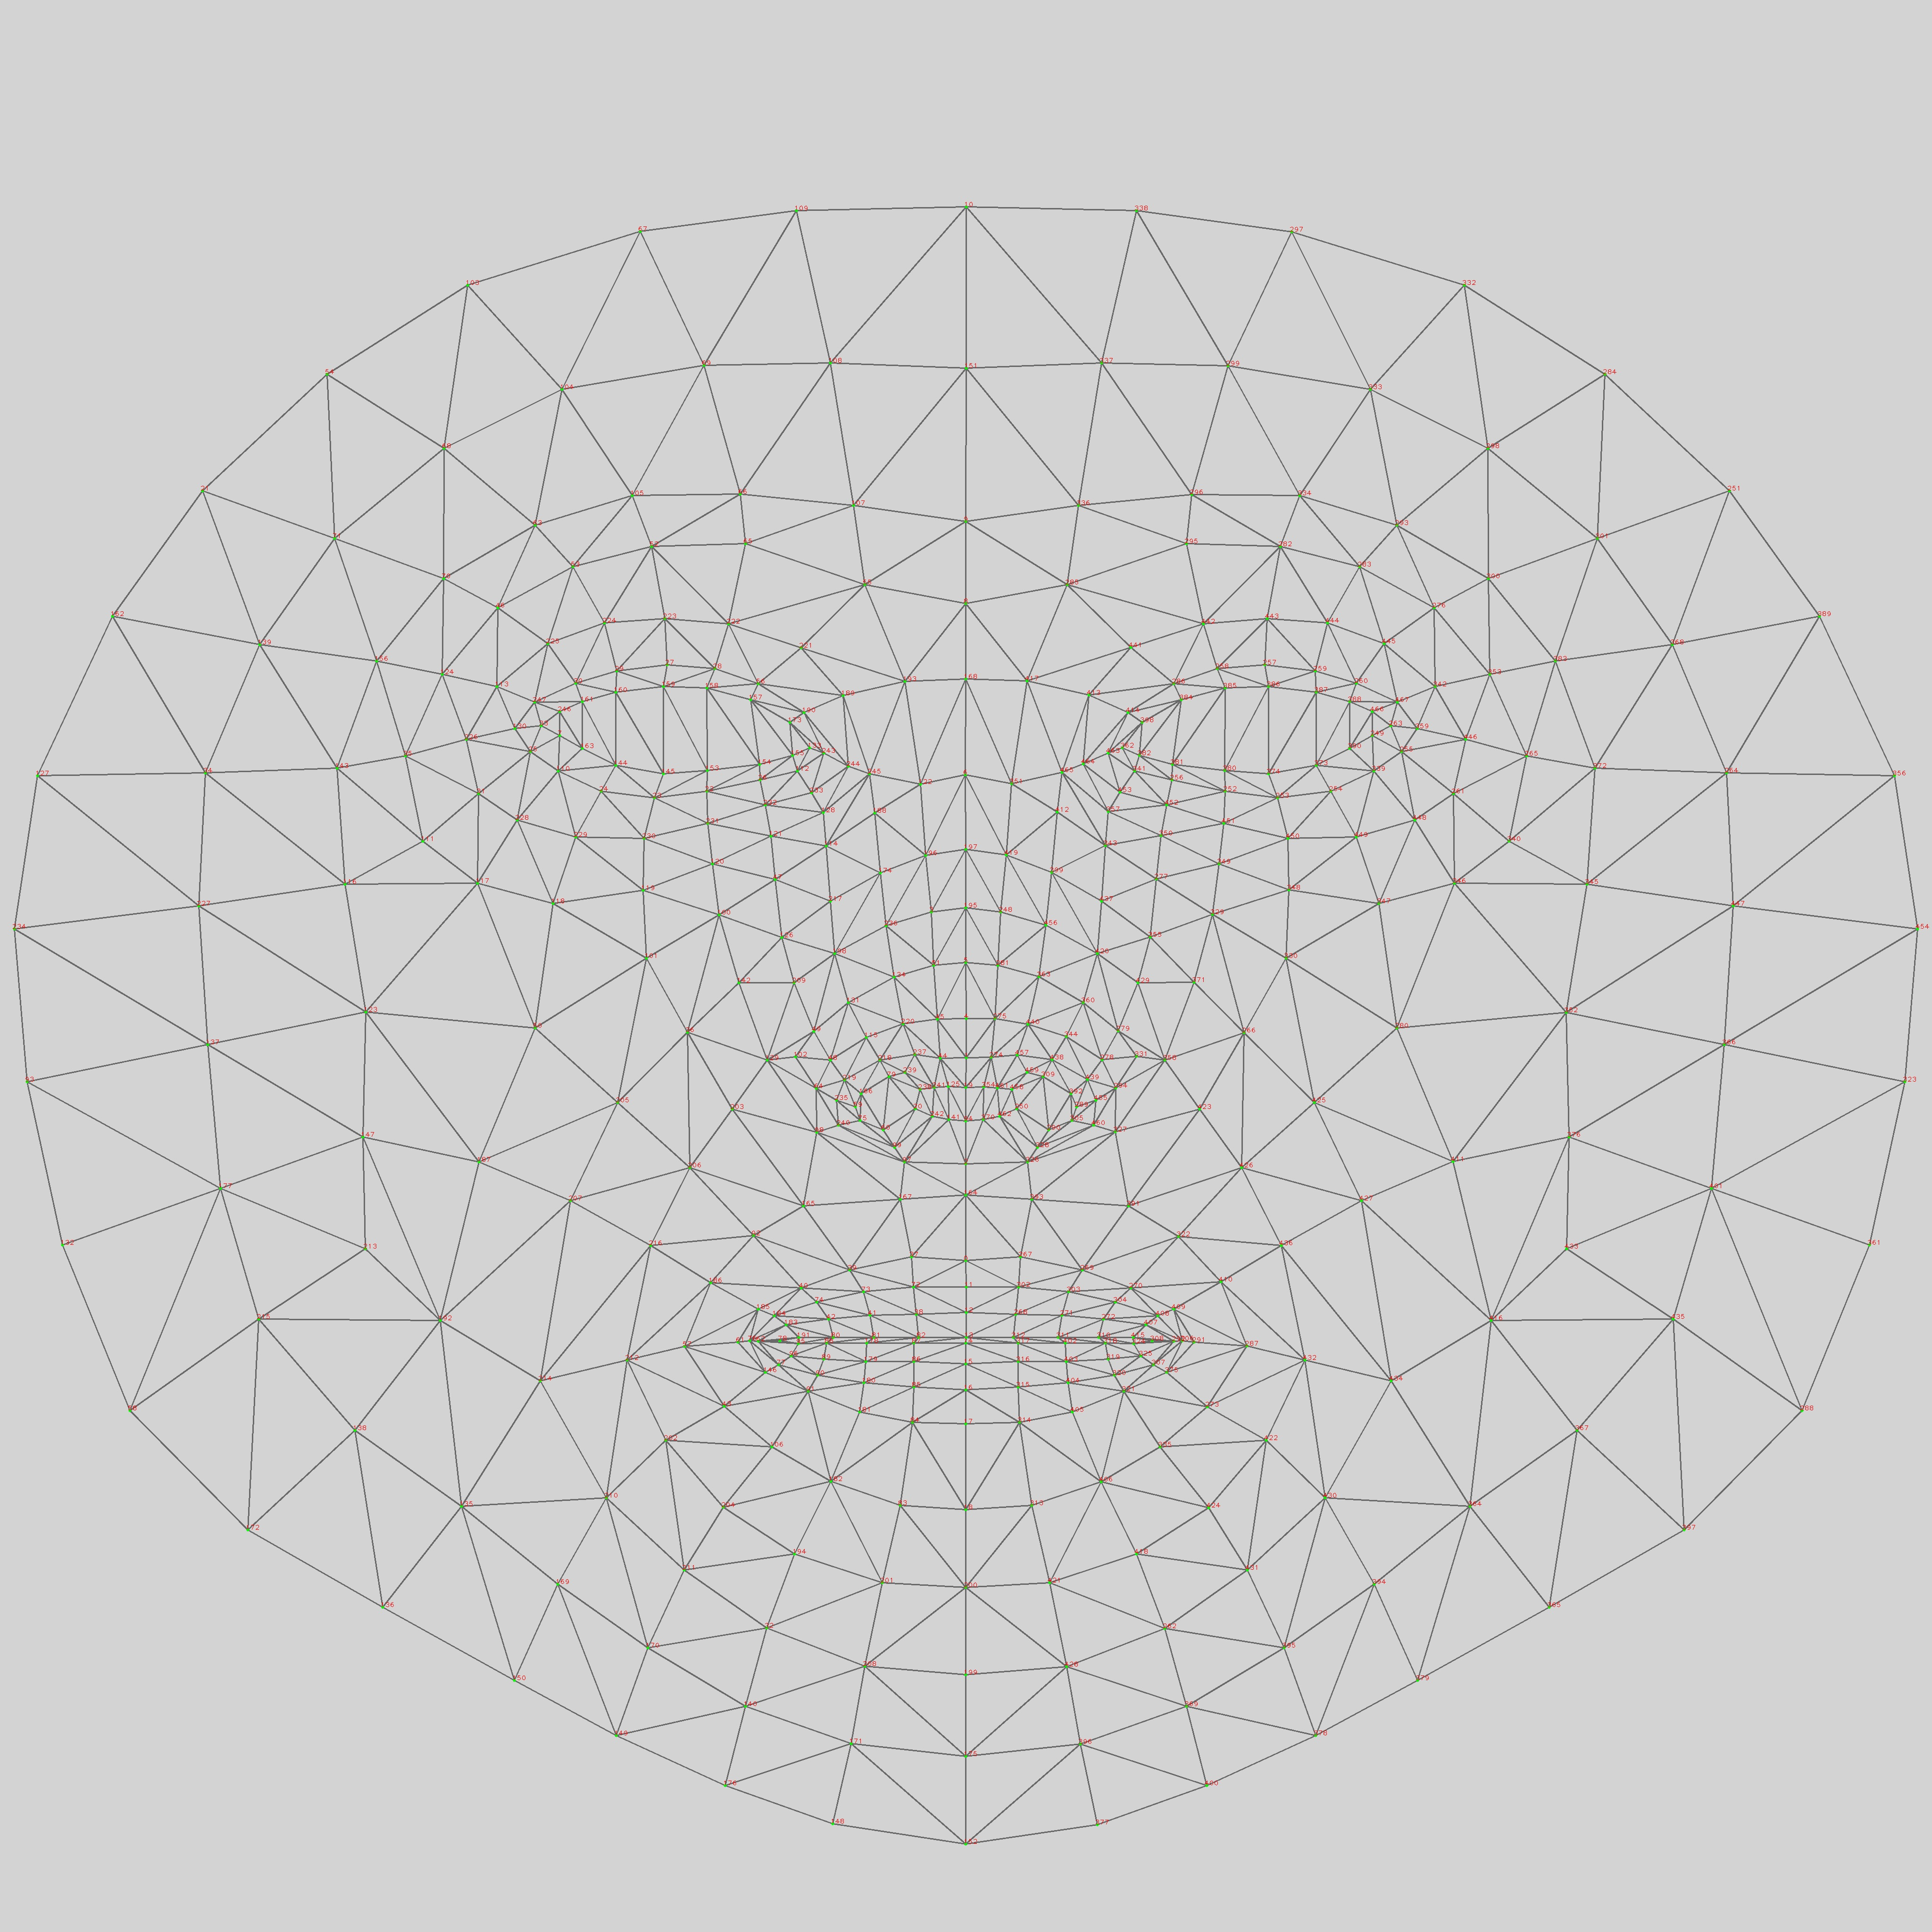
\includegraphics[width=0.75\linewidth]{img/facemesh-kepyoints.jpg}
        \caption{\textit{Output} del modelo de \textit{facemesh} utilizado por
        \texttt{WebGazer} para la localización de los ojos}
      \end{figure}
    \end{column}
  \end{columns}

\end{frame}

\begin{frame}{Calibración y validación}
  \begin{itemize}
    \item Nuestro caso de uso no garantiza interacciones

    \item Se muestran una serie de puntos, para cada uno de los cuales el
      usuario tendrá que fijar la mirada y presionar la barra de espacio
    
    \item Validación post calibración implementada de similar manera

    \item[\emoji{party-popper}] \texttt{WebGazer} adaptado para evitar cómputos
      ya no necesarios
  \end{itemize}
\end{frame}

\begin{frame}{Notificación de descalibración}

  \begin{columns}
    \begin{column}{.5\textwidth}
      \begin{itemize}
        \item Basada en detectar movimiento
        \item Instanciada luego de cada calibración
        \item Verificación realizada para cada \textit{frame}
        \item \emoji{party-popper} \texttt{WebGazer} adaptado para exponer los
          recuadros calculados en cada \textit{frame} por la rutina de
          localización de ojos
      \end{itemize}
    \end{column}

    \begin{column}{.5\textwidth}
      \begin{figure}
        \centering
        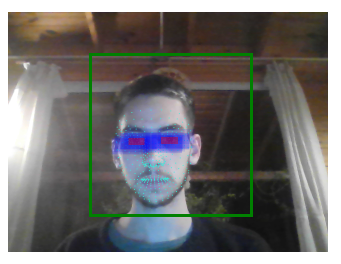
\includegraphics[width=\textwidth]{img/eyetracker-playground-screenshot.png}
        \caption{Detección de movimiento en funcionamiento}
      \end{figure}
    \end{column}
  \end{columns}

\end{frame}

\section{Experimentación}

\begin{frame}{Caso de estudio: tarea de antisacadas}

  \begin{columns}
    \begin{column}{.5\textwidth}
      \begin{itemize}
        \item Clínicamente relevante
        \item Resultados esperados ya establecidos
        \item Tarea simple para validar movimientos oculares
      \end{itemize}
    \end{column}
    \begin{column}{.5\textwidth}
      \begin{figure}
        \centering
        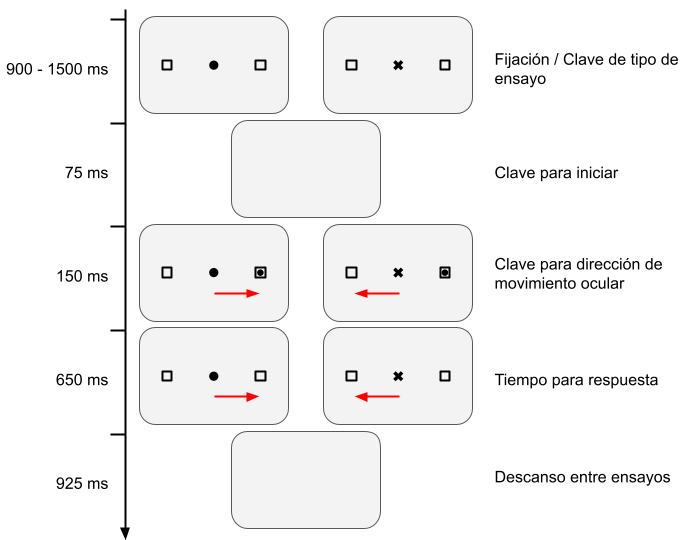
\includegraphics[width=\linewidth]{img/antisaccades-protocol.png}
        \caption{Protocolo de las tareas}
      \end{figure}
    \end{column}
  \end{columns}

\end{frame}

\begin{frame}{Primera instancia}
  \begin{itemize}
    \item Limitados a 10 minutos debido a una falla de \texttt{WebGazer}
    \item Únicamente ensayos de antisacada
    \item Recalibración luego de cada notificación de descalibración
    \item Sin validación post calibración
  \end{itemize}
\end{frame}

\begin{frame}{Segunda instancia}
  \begin{itemize}
    \item Duración superior a 20 minutos
    \item Ensayos de prosacadas y de antisacadas
    \item Recalibración cada 10 ensayos y sólo si se detectó una
      descalibración
    \item Con validación post calibración
  \end{itemize}
\end{frame}

\begin{frame}{Implementación y distribución}

  \begin{columns}
    \begin{column}{0.4\textwidth}
      \begin{figure}
        \centering
        
\includegraphics[width=\textwidth]{img/jspsych-logo.jpg}
      \end{figure}
    \end{column}
    \begin{column}{0.6\textwidth}
      \begin{figure}
        \centering
        
\includegraphics[width=0.8\textwidth]{img/cognition-run-logo.png}
        
\includegraphics[width=\textwidth]{img/neuropruebas-logo.jpg}
      \end{figure}
    \end{column}
  \end{columns}
\end{frame}


\section{Resultados}

\begin{frame}{Ejemplo de \textit{output} del sistema}
  \begin{figure}
    \centering
    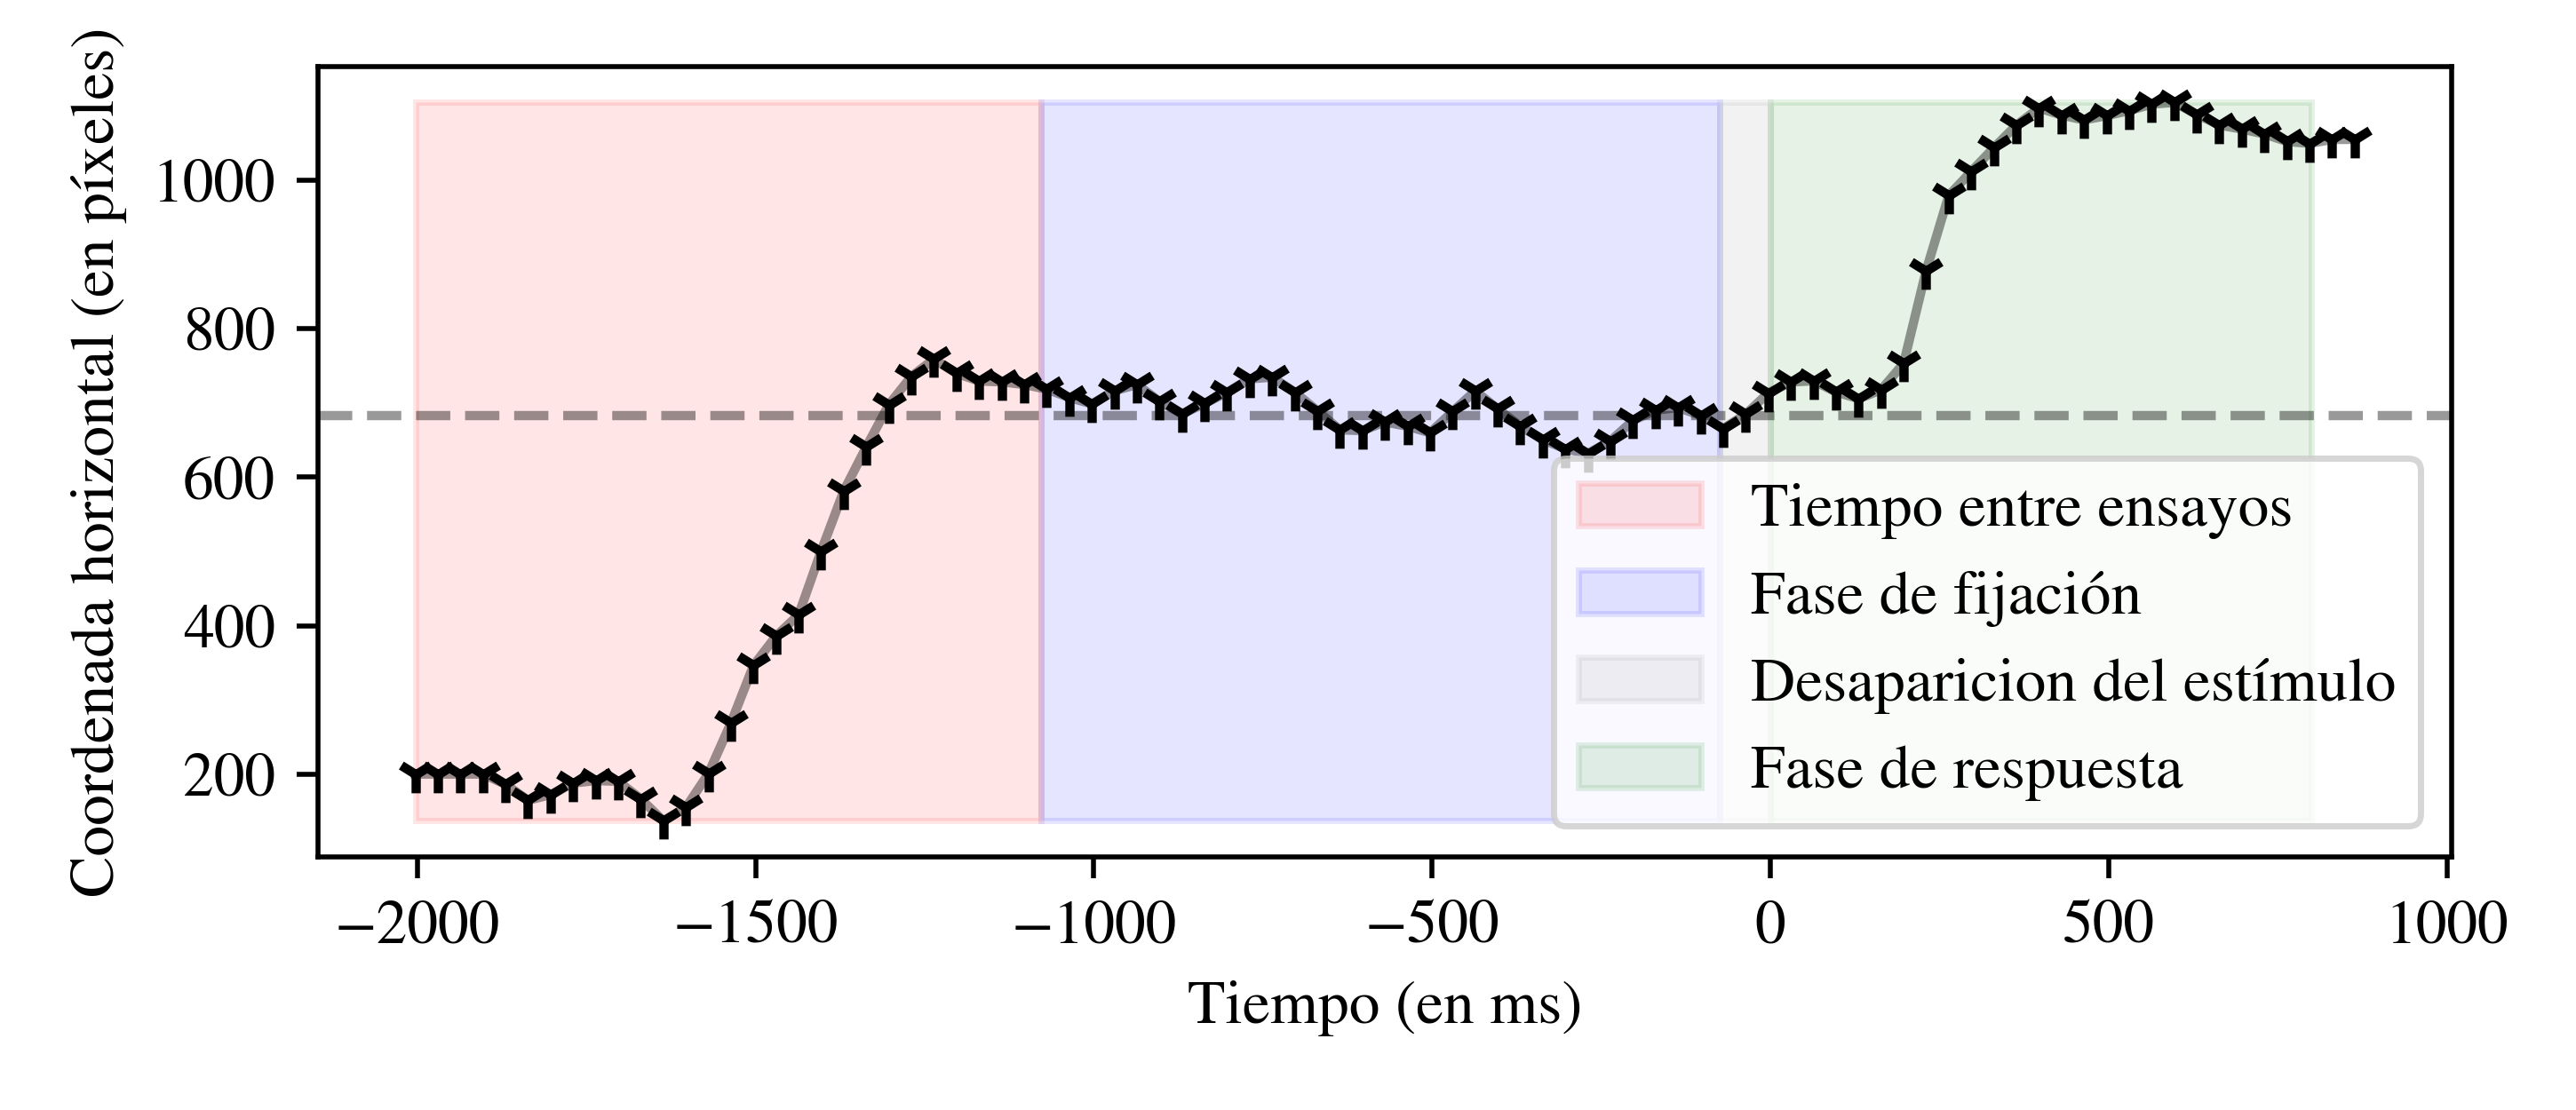
\includegraphics[width=\linewidth]{plots/output-example.png}
  \end{figure}
\end{frame}

\begin{frame}{Frecuencias de muestreo}
  \begin{figure}
    \centering
    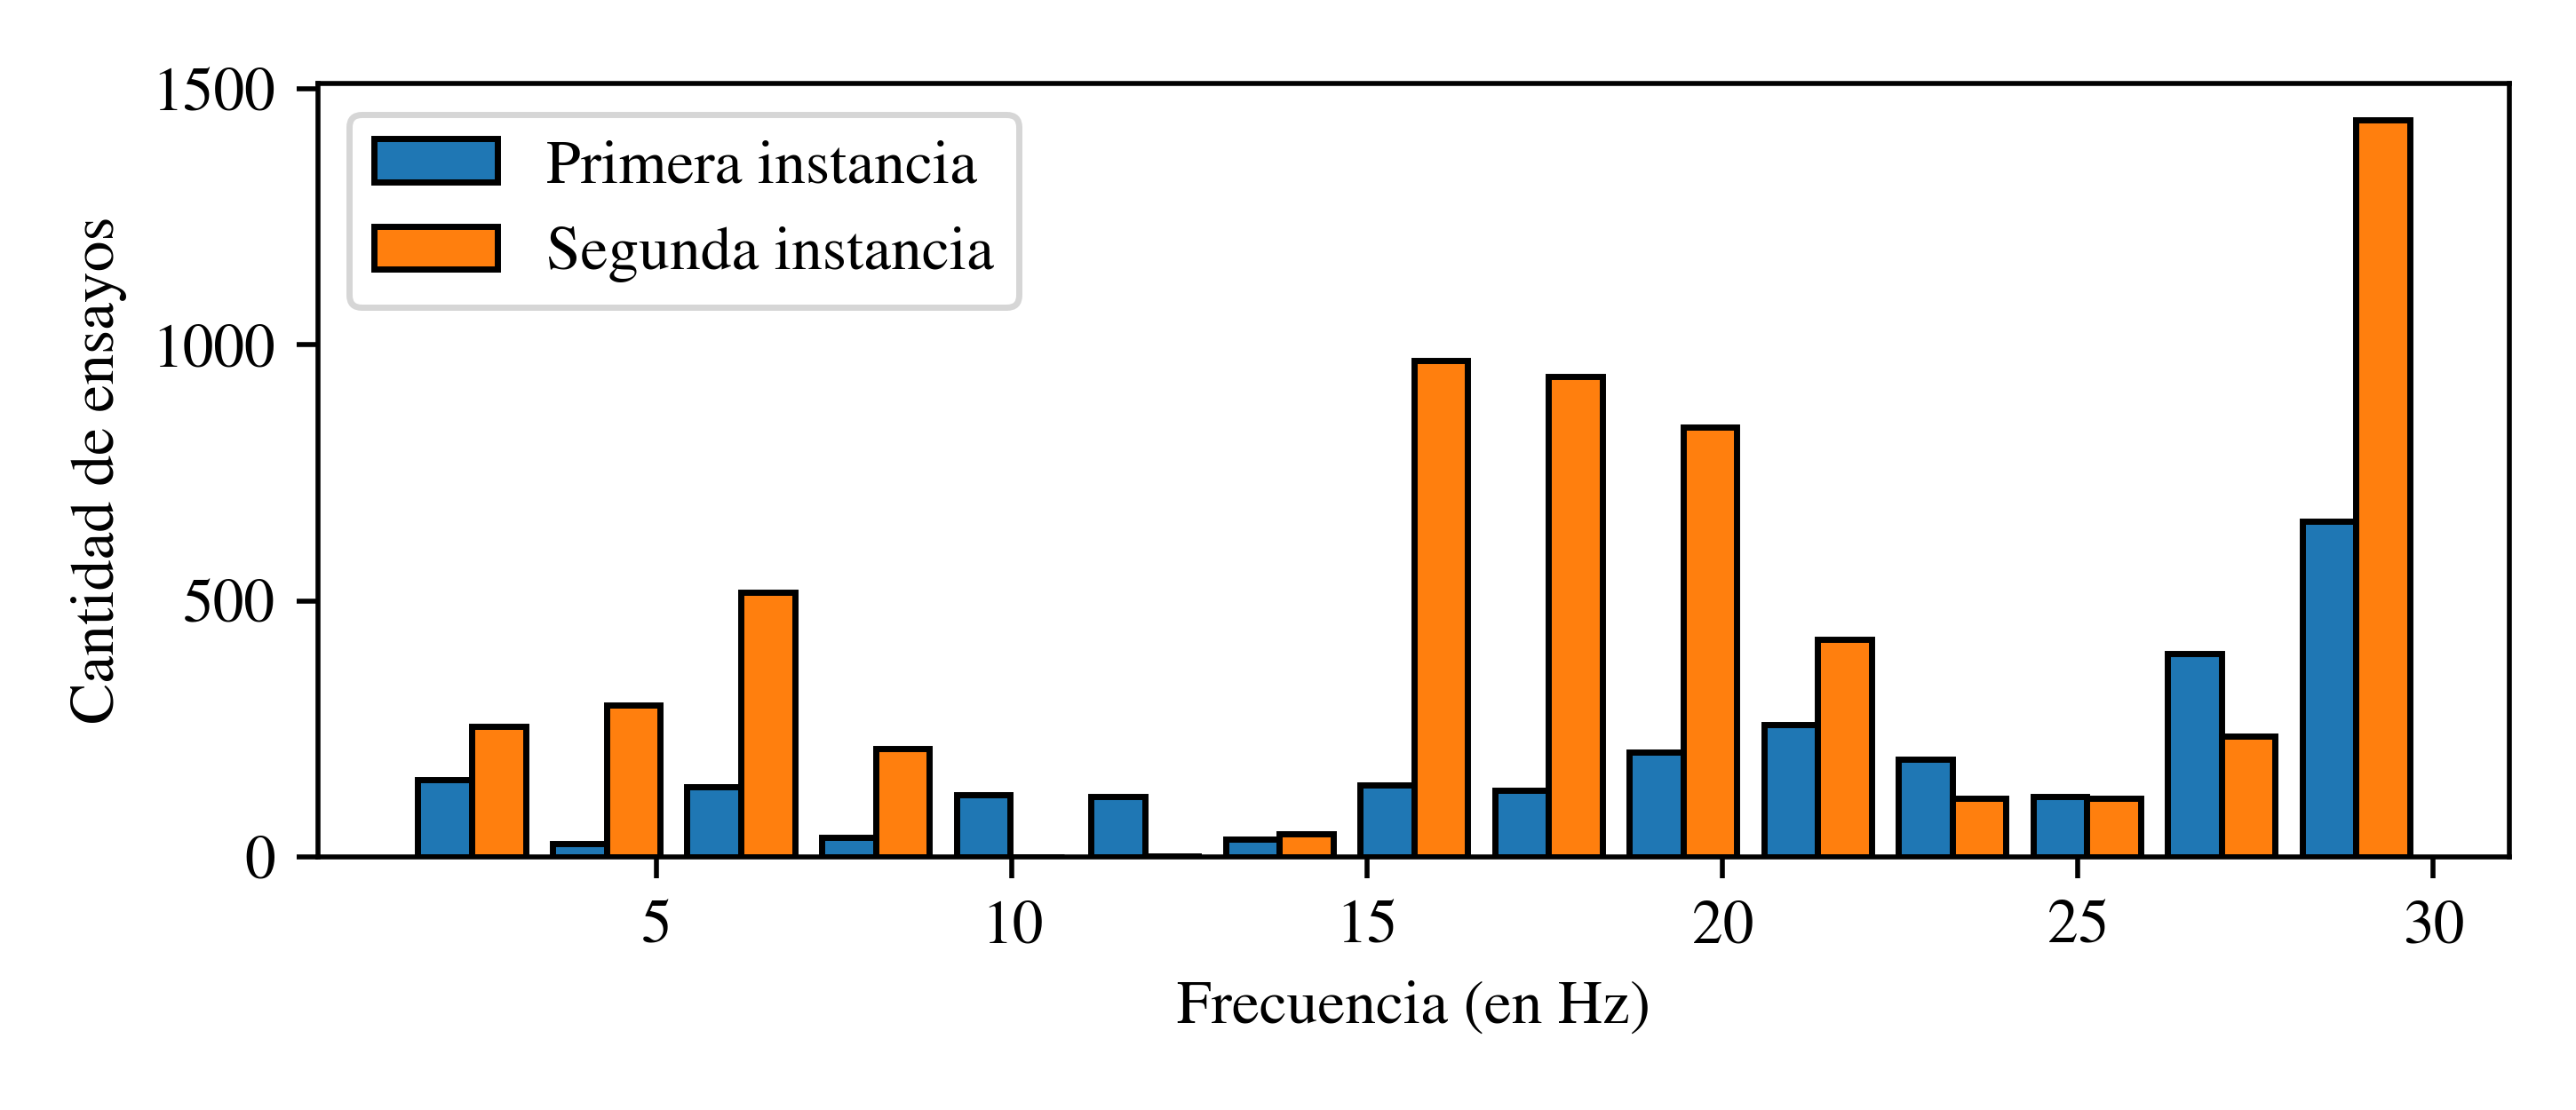
\includegraphics[width=\linewidth]{plots/sampling-frequencies-distribution.png}
  \end{figure}
\end{frame}

\begin{frame}{Anchos de pantalla}
  \begin{figure}
    \centering
    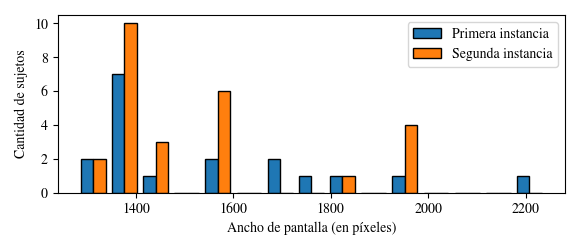
\includegraphics[width=\linewidth]{plots/screens-widths-distribution.png}
  \end{figure}
\end{frame}

\begin{frame}{Estimaciones desviadas}
  \begin{figure}
    \centering
    \includegraphics[width=\linewidth]{plots/skewed-estimations-examples.png}
    \caption{Las estimaciones de algunos sujetos están desviadas de los valores reales}
  \end{figure}
\end{frame}

\begin{frame}{Limpieza y normalización}
  \begin{columns}
    \begin{column}{0.4\textwidth}
      \begin{itemize}
        \item Ensayos descartados: \begin{itemize}
          \item frecuencia menor a 15 Hz
          \item a mano
          \item si el sujeto se distrajo de la tarea
        \end{itemize}
        \item Frecuencia de muestreo: \textit{Upsampling} a 30 Hz usando
          interpolación lineal
      \end{itemize}
    \end{column}
    \begin{column}{0.6\textwidth}
      \begin{figure}
        \centering
        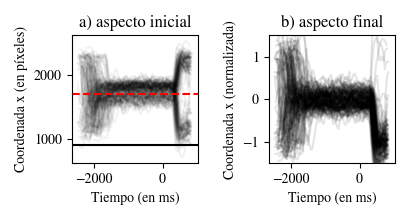
\includegraphics[width=\linewidth]{plots/normalization-example.png}
        \caption{Normalizado y espejado}
      \end{figure}
    \end{column}
  \end{columns}
\end{frame}

\begin{frame}{Detección de sacadas}
  \begin{columns}
    \begin{column}{0.5\textwidth}
      \begin{figure}
        \centering
        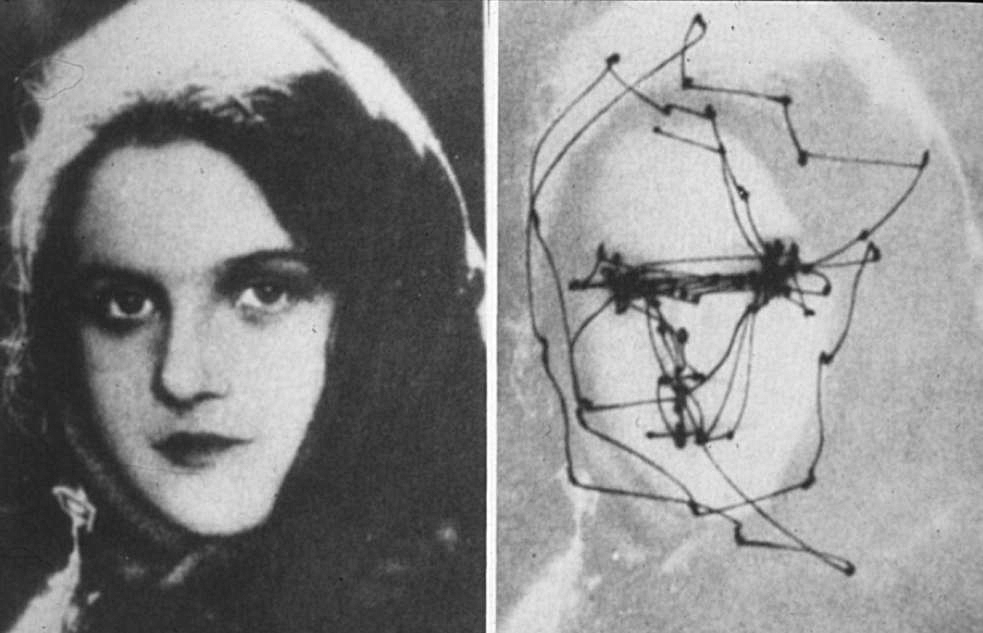
\includegraphics[width=\linewidth]{img/saccades-example.jpg}
        \caption{Los movimientos oculares muestran qué elementos de una imagen
        capturan la atención}
      \end{figure}
    \end{column}
    \begin{column}{0.5\textwidth}
      \begin{figure}
        \centering
        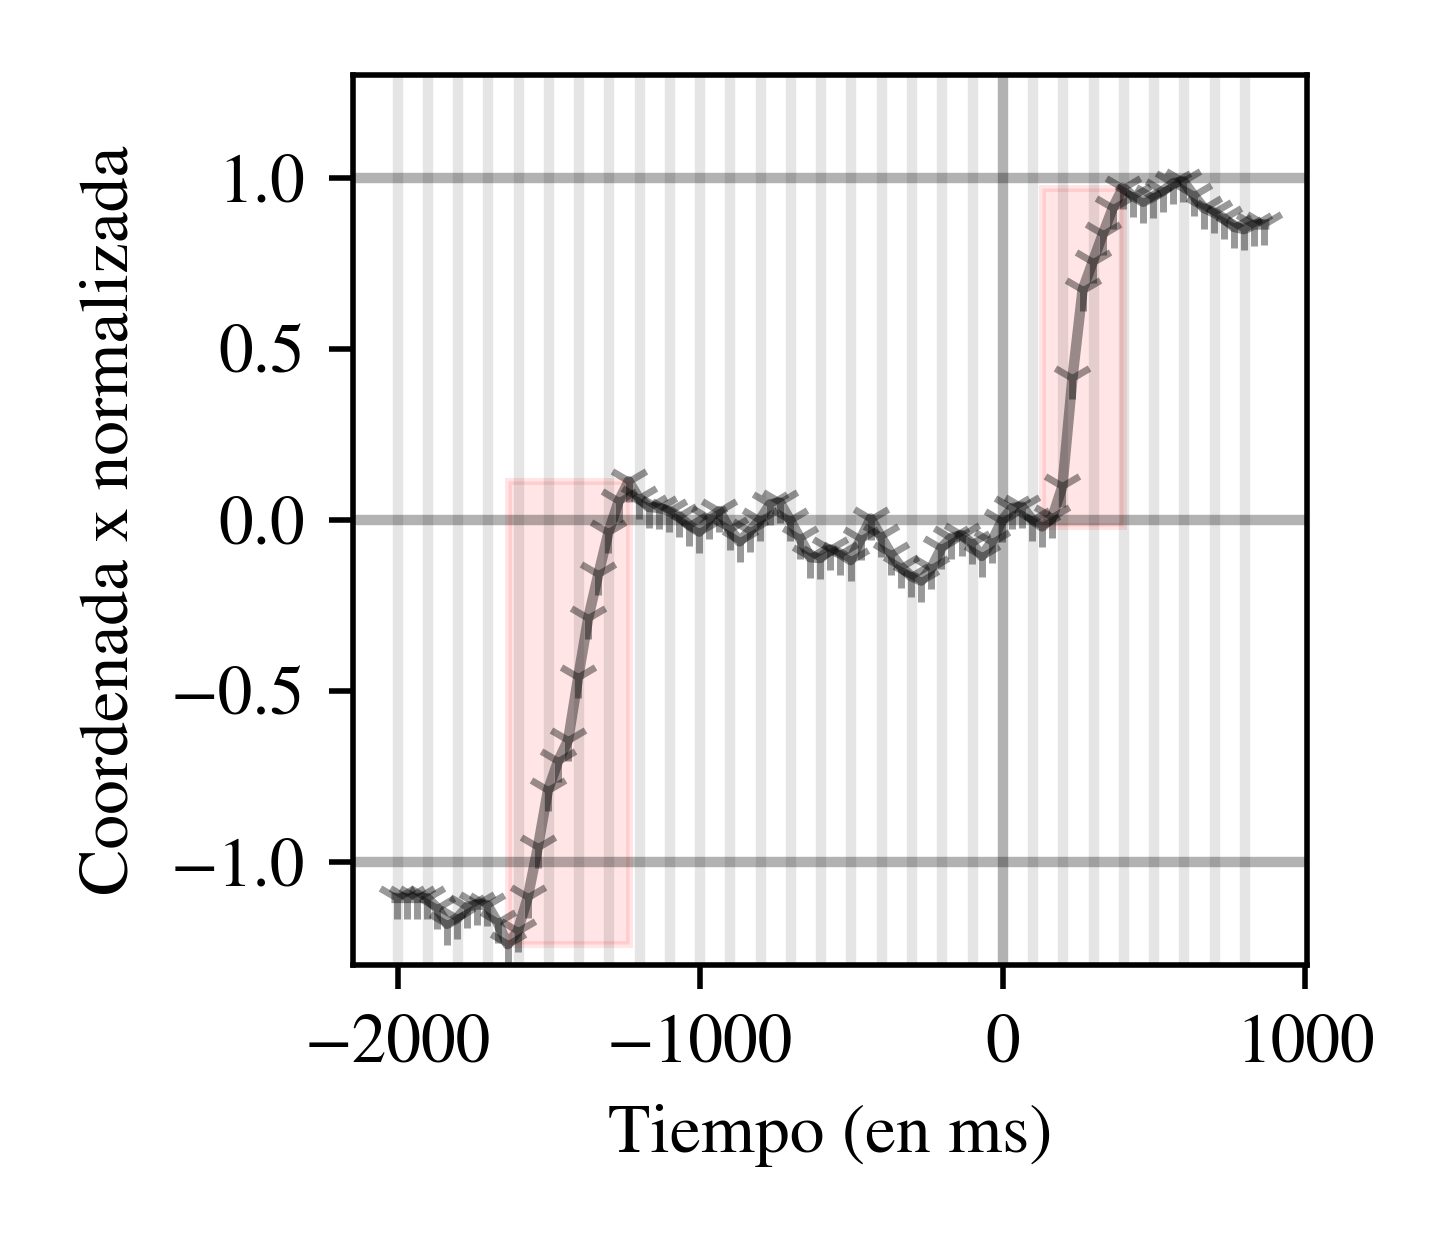
\includegraphics[width=\linewidth]{plots/detected-saccades-example.png}
        \caption{Sacadas detectadas sobre las estimaciones de un ensayo}
      \end{figure}
    \end{column}
  \end{columns}
\end{frame}

\begin{frame}{Conclusiones generales replicadas}
  \begin{table}
    \centering
    \begin{tabular}{ l | c | c | c }
      & correctitud & \multicolumn{2}{ c }{tiempo de respuesta (ms)} \\
      &             & correcto & incorrecto \\
      \hline
      antisacada & 81.29\% & 509 (93) & 346 (105) \\
    \end{tabular}
    \caption{Primera instancia}
  \end{table}
  
  \begin{table}
    \centering
    \begin{tabular}{ l | c | c | c }
      & correctitud & \multicolumn{2}{ c }{tiempo de respuesta (ms)} \\
      &             & correcto & incorrecto \\
      \hline
      antisacada & 94.82\% & 358 (109) & 299 (103) \\
      \hline
      prosacada & 98.09\% & 320 (108) & 311 (150) \\
    \end{tabular}
    \caption{Segunda instancia}
  \end{table}

  % TODO: Poner marker negativo acá
  En la bibliografía para la tarea de antisacadas se reportan \textbf{valores
  de correctitud} más cercanos al rango $[60\%, 75\%]$.
\end{frame}

\begin{frame}{Menos datos de lo esperado}
  \begin{columns}
    \begin{column}{0.4\textwidth}
      \begin{itemize}
        \item Cantidad de ensayos iniciales baja en relación a otros trabajos
        \item Descarte de aproximadamente $\frac{2}{3}$ de los datos
        \item Altas e inesperadas tasas de correctitud
      \end{itemize}
    \end{column}

    \begin{column}{0.6\textwidth}
      \begin{table}
        \centering

        \begin{tabular}{ l | c | c }
          Antisacadas   & incorrecto  & correcto \\
          \hline
          \# total      & 64          & 1173 \\
          \hline
          \# por sujeto & 4.57 (2.84) & 78.20 (40.38)
        \end{tabular}

        \vspace{0.3cm}

        \begin{tabular}{ l | c | c }
          Prosacadas    & incorrecto  & correcto \\
          \hline
          \# total      & 22          & 1134 \\
          \hline
          \# por sujeto & 2.44 (1.23) & 75.59 (38.58)
        \end{tabular}

        \caption{Desbalance entre grupos incorrecto y grupo correcto}
      \end{table}
    \end{column}
  \end{columns}
\end{frame}

\begin{frame}{~}
  fin
\end{frame}

\section{Motivación}

\begin{frame}{~}

  \begin{itemize}
      \item Los ojos como entrada a los procesos cognitivos y estados
        emocionales de una persona
      \item Frecuentemente estudiados en el contexto de la neuropsicología
        digital para estimar el comportamiento
      \item Importante incluso cuando no son el foco del análisis
        (\textit{e.g.}, detección de caras)
      % utilizado también en el desarollo HMI, en el estudio de usabilidad de
      % interfaces, recientemente en el campo de la oftalmología para estimar
      % el campo visual
      \item Usos en otras disciplinas
  \end{itemize}

  \begin{figure}
    \begin{subfigure}{0.49\textwidth}
      \centering
      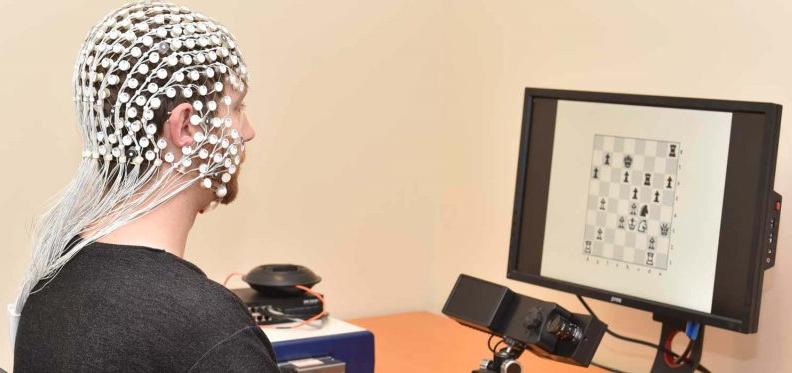
\includegraphics[width=\linewidth]{img/eye-link-eeg.jpg}
      \caption{\textit{Eye tracking} combinado con electroencefalograma}
    \end{subfigure}
    \begin{subfigure}{0.49\textwidth}
      \centering
      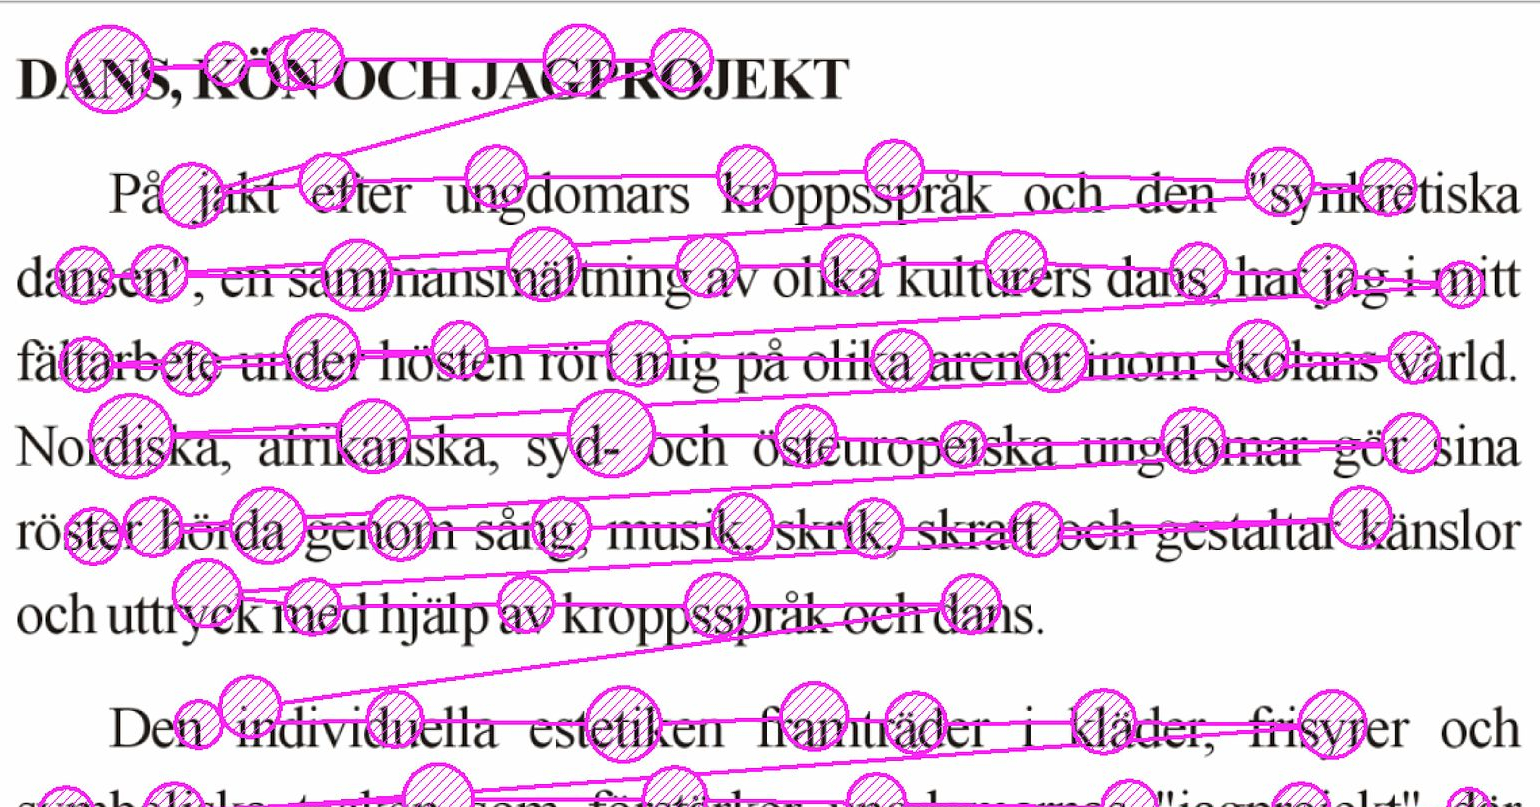
\includegraphics[width=\linewidth]{img/reading-fixations-saccades.jpg}
      \caption{Estimación de la mirada durante una tarea de lectura}
    \end{subfigure}
  \end{figure}

\end{frame}

\begin{frame}{~}

  \begin{itemize}
    \item Comunmente resuelto con sistemas comerciales cerrados
    \item Costos altos (entre 5000 y 40000 euros) mientras que el hardware en
      sí representa una pequeña fracción de estos (entre 200 y 600 euros)

    % si falta algún dato (e.g., la precisión del diámetro de la pupila) no
    % se lo puede saber
    \item Imposibilidad de auditar la implementación
    \item Necesidad de asistir a un laboratorio
  \end{itemize}

  \begin{figure}
    \begin{subfigure}{0.49\textwidth}
      \centering
      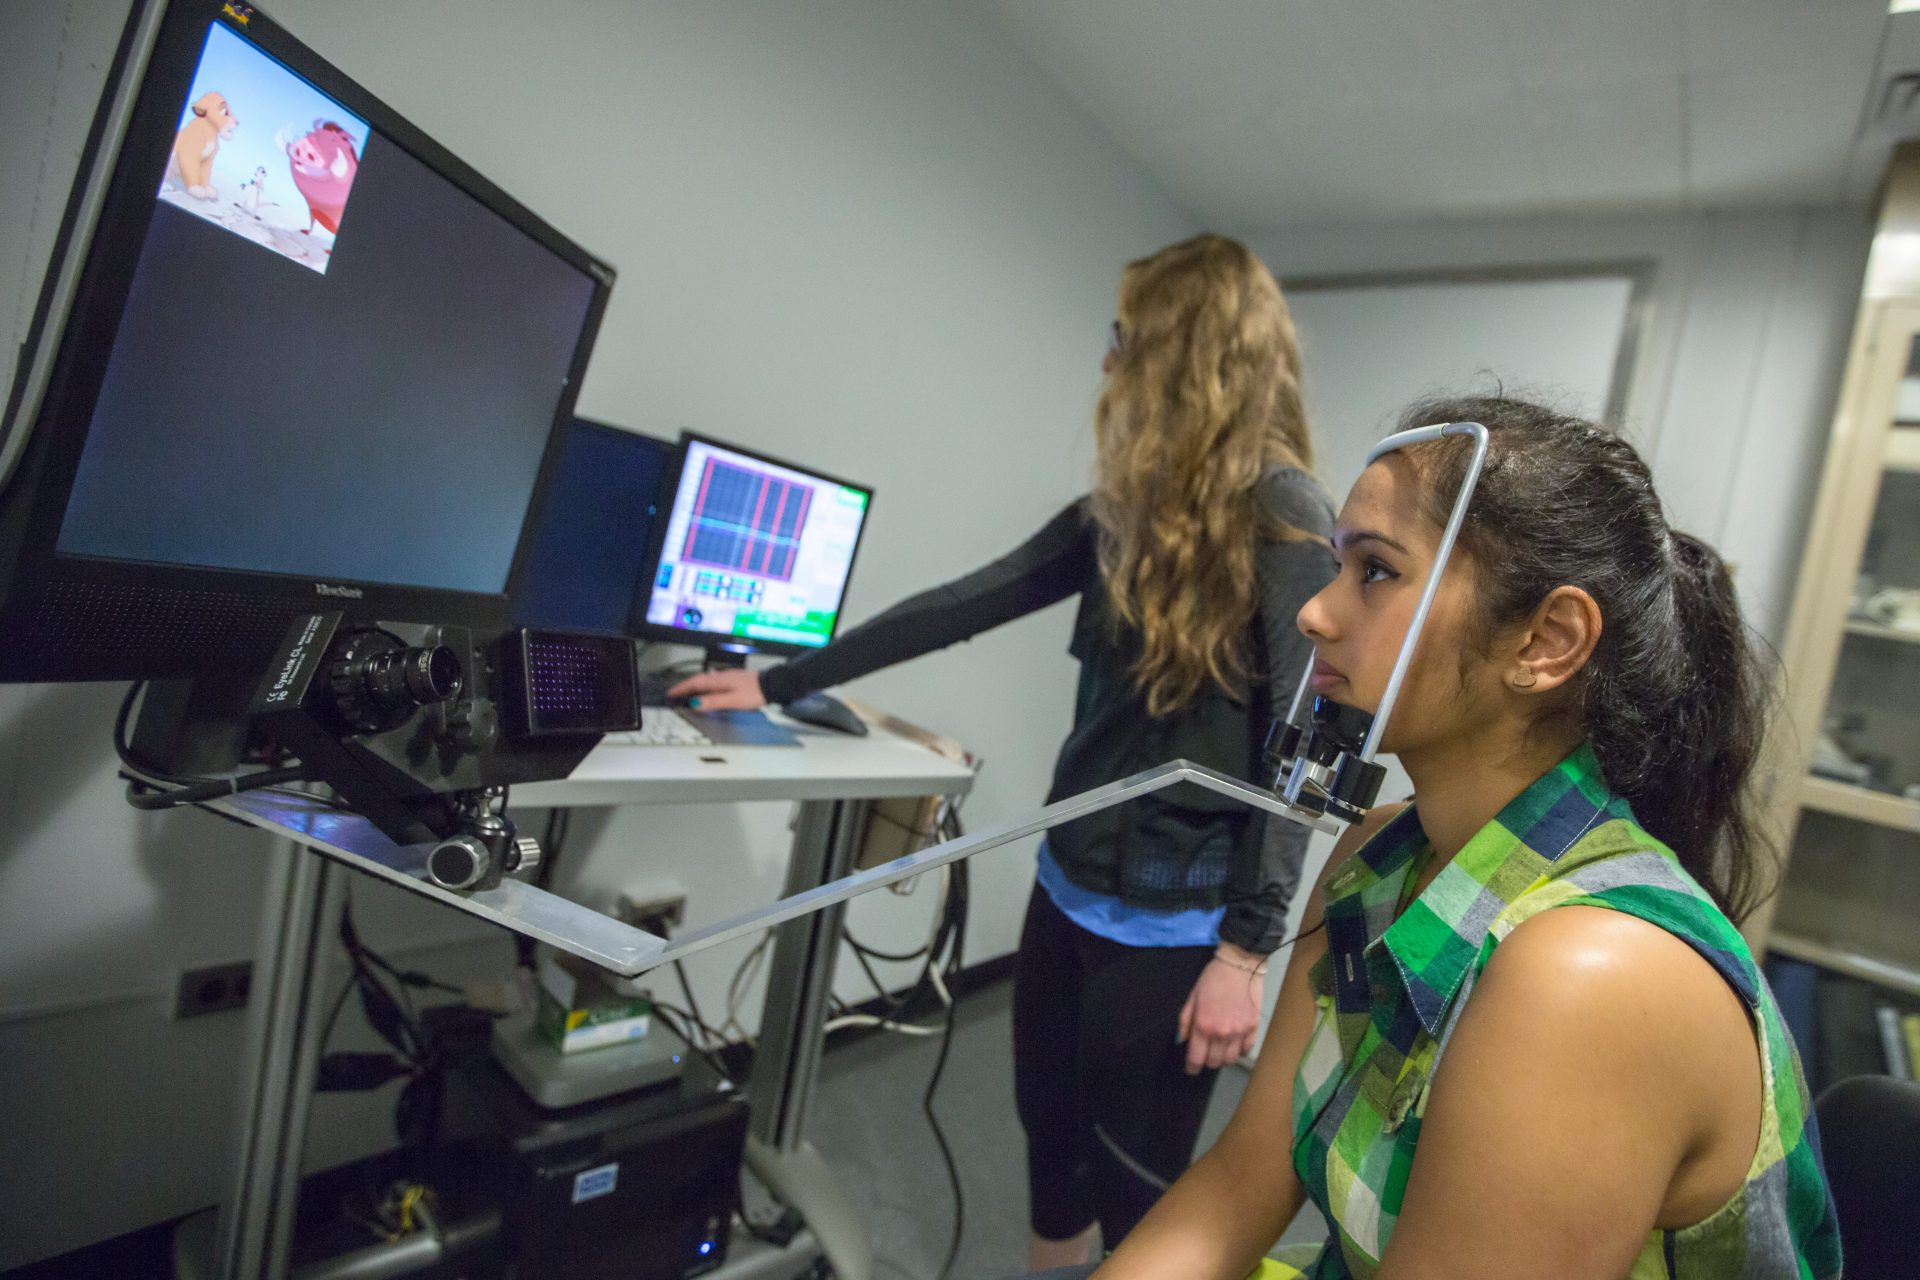
\includegraphics[width=0.6\linewidth]{img/eye-link-chinrest.jpg}
      \caption{La reestricción de movimiento facilita mantener calibrado el
      sistema}
    \end{subfigure}
    \begin{subfigure}{0.49\textwidth}
      \centering
      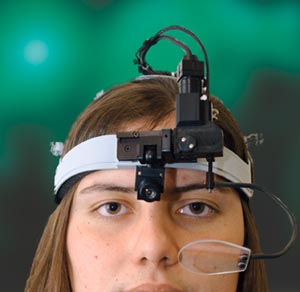
\includegraphics[width=0.5\linewidth]{img/eye-tracker-head-mounted.jpg}
      \caption{\textit{Eye tracker} montado a la cabeza}
    \end{subfigure}
  \end{figure}

\end{frame}

\begin{frame}{~}

  \begin{columns}
    \begin{column}{0.4\textwidth}
      \begin{itemize}
        \item Interés en proveer software de \textit{eye tracking}

        \item Posibilidad de \textit{crowdsourcing}

          % e.g., detectar pérdidas de atención en clases masivas
        \item Potencial para nuevas aplicaciones
      \end{itemize}

    \end{column}
    \begin{column}{0.6\textwidth}

      \begin{figure}
        \begin{subfigure}{0.49\textwidth}
          \centering
          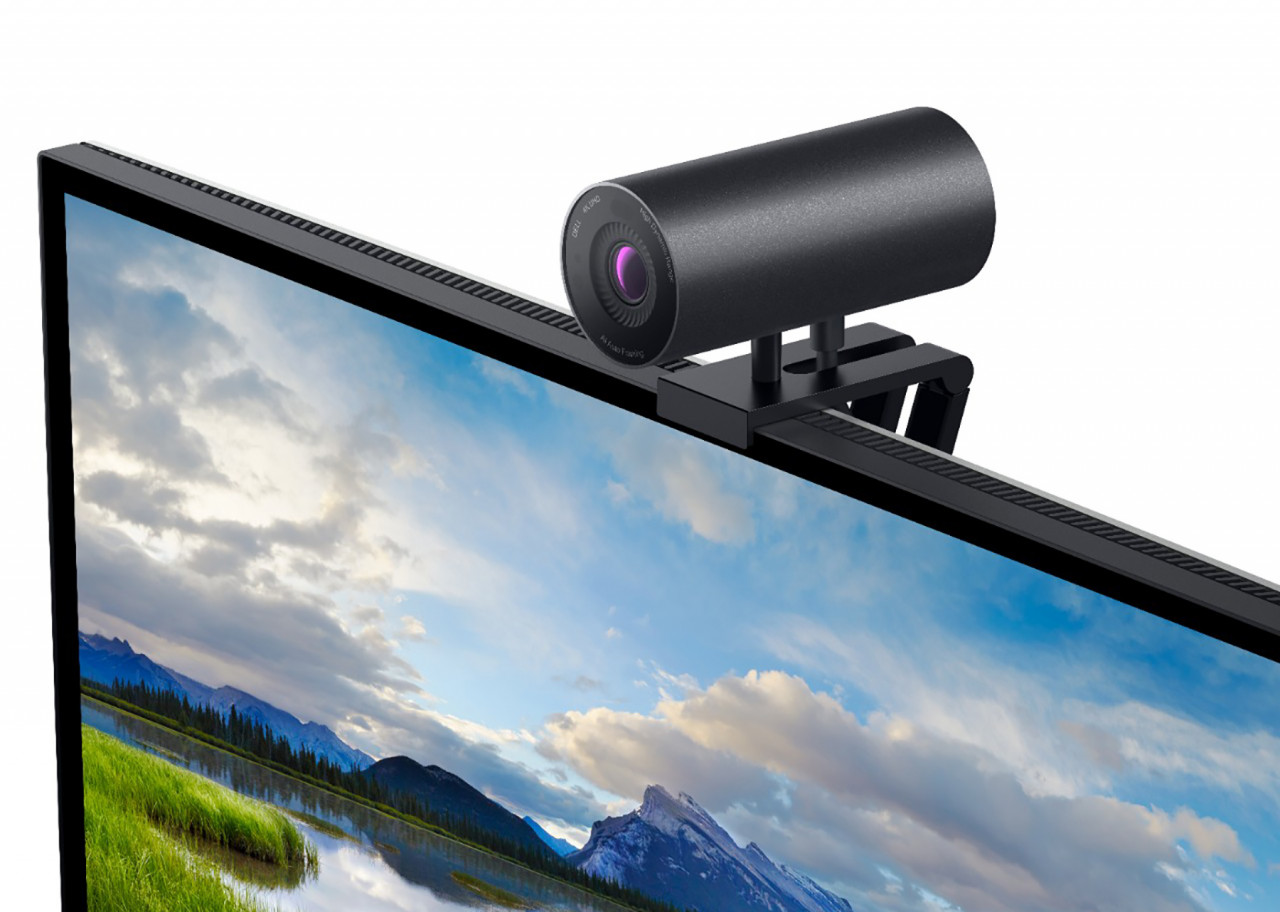
\includegraphics[width=0.8\linewidth]{img/external-webcam.jpg}
        \end{subfigure}
        \begin{subfigure}{0.49\textwidth}
          \centering
          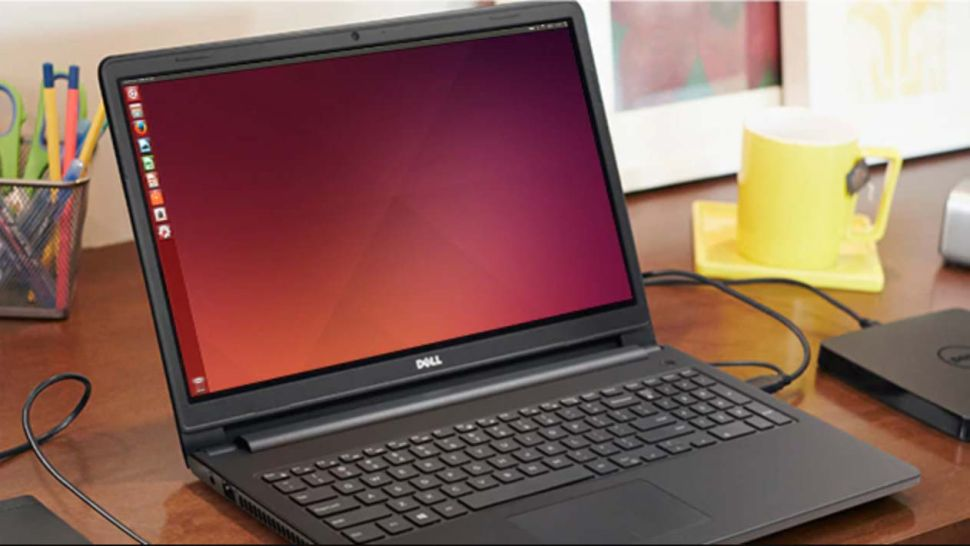
\includegraphics[width=0.8\linewidth]{img/notebook.jpg}
        \end{subfigure}
        \caption{Webcams domésticas ya disponibles}
      \end{figure}

      \begin{figure}
        \begin{subfigure}{0.49\textwidth}
          \centering
          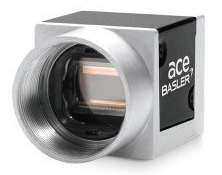
\includegraphics[width=0.6\linewidth]{img/basler-camera.jpg}
        \end{subfigure}
        \begin{subfigure}{0.49\textwidth}
          \centering
          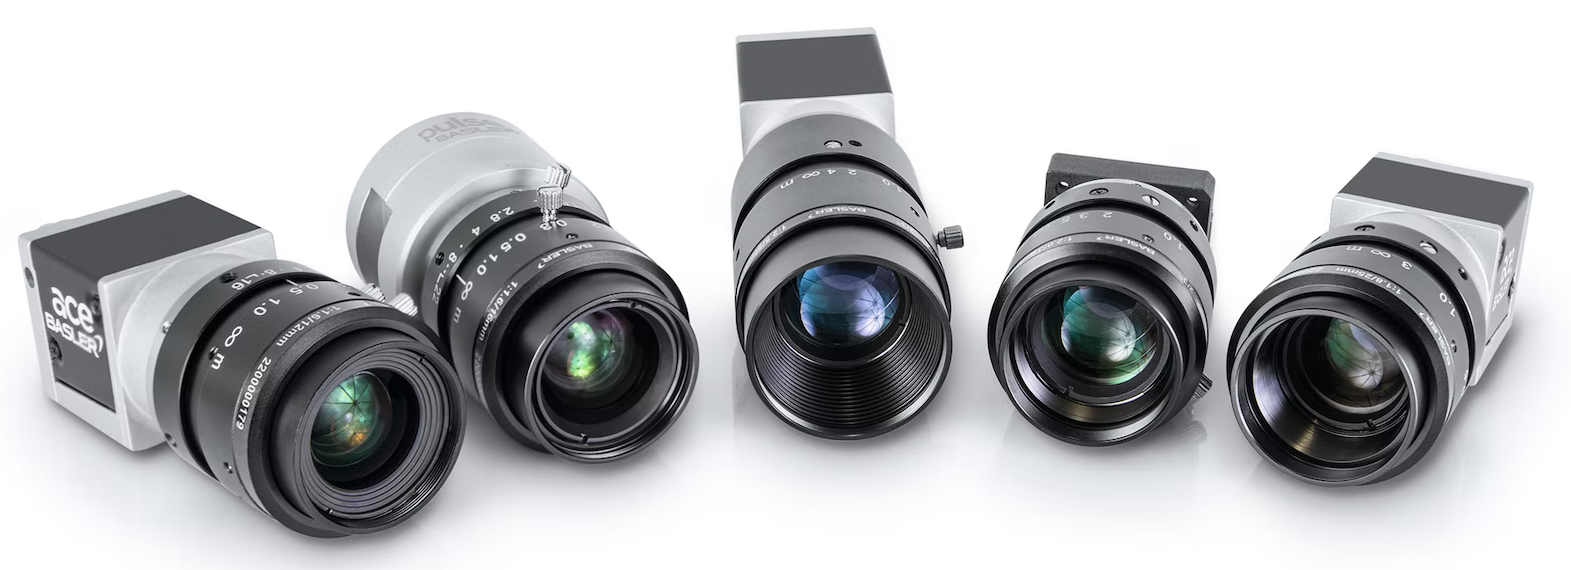
\includegraphics[width=0.8\linewidth]{img/basler-cameras-with-lens.png}
        \end{subfigure}
        \caption{Hardware profesional adquirible por una fracción del costo}
      \end{figure}


    \end{column}
  \end{columns}
\end{frame}

\section{Objetivos}

\begin{frame}{~}

  \begin{itemize}
    \item Evaluar implementaciones recientes con similares motivaciones
    % - entender el problema
    % - definir los requerimientos
    % - establecer qué puede reutilizarse

    \item Implementar un prototipo de \textit{eye tracker} que corra en
      navegadores \textit{web} y que esté orientado a análisis clínicos
    % - adaptar lo que pudiera reutilizarse
    % - implementar los módulos que faltaran

    \item Emular análisis clínicos remotos y recolectar datos utilizando el
      prototipo implementado

    \item Establecer la capacidad del prototipo en replicar conclusiones
      establecidas con \textit{eye trackers} profesionales de laboratorio

  \end{itemize}

\end{frame}

\section{Desarmando el problema de \textit{eye tracking} web}

\begin{frame}{~}
  \begin{columns}
    \begin{column}{0.5\textwidth}
      \begin{itemize}
        \item Estimar qué coordenada de la pantalla está mirando el usuario en
          un contexto de estudios clínicos
        \item Un \textit{stream} de frames de la webcam como \textit{input}
        \item Se divide en \textbf{localizar los ojos} y luego \textbf{estimar
          la mirada}
        \item Calibraciones necesarias en cada sesión de uso
      \end{itemize}
    \end{column}
    \begin{column}{0.5\textwidth}
      \begin{figure}
        \centering
        TODO: Reemplazar esto por un único plot que ejemplifique el output
        deseado
        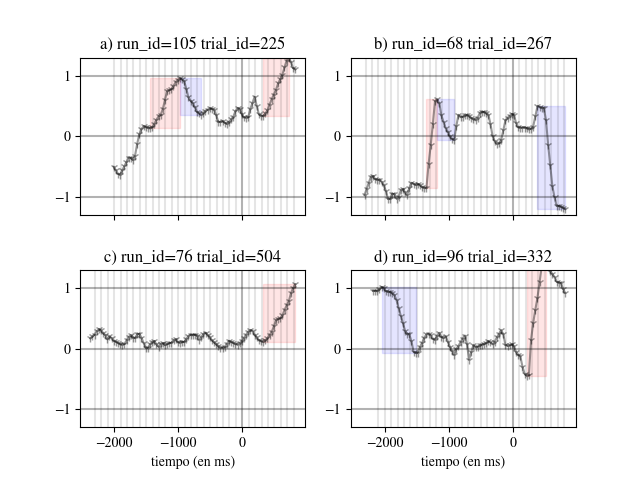
\includegraphics[width=\linewidth]{img/eye-tracking-output-example.png}
        \caption{Sacadas detectadas sobre serie de tiempo de la coordenada x}
      \end{figure}
    \end{column}
  \end{columns}
\end{frame}

\begin{frame}{~}
    \begin{itemize}
    \item Resultados consistentes dentro de una misma población
    % - mayor tasa de correctitud para los casos de prosacada que para aquellos de antisacada
    % - para los grupos correctos se esperan mayores tiempos de respuesta en las repeticiones de antisacadas que en aquellas de prosacadas
    % - a mayor edad menor rendimiento en la tarea, tanto en latencia como en correctitud

    \item Búsqueda de establecer resultados para poblaciones de distinta condición neuropsicológica
    % - ditintos tipos de lesiones cerebrales
    % - déficit de atención, esquizofrenia, síndrome de Parkinson, síndrome de Tourette
    % - individuos sanos, efectos de la edad

    \item Comparación dificultosa entre distintos trabajos
    % - se obtienen valores del mismo orden (RT y correctitud) para pacientes sanos en un estudio que para pacientes con esquizofrenia de otro estudio
    \end{itemize}

\end{frame}

\section{Alternativas al \textit{eye tracking} tradicional}

\subsection{Trabajos previos}

\begin{frame}{~}

  TODO: Separar esto en varios frames
  \begin{itemize}
    \item \texttt{PupilEXT}: software para realizar pupilometría; deben
      proveerse cámaras profesionales y emisores de luz infrarroja; TODO:
      imagen pupilometría

    % hay que resaltar la importancia de esto de analizar el momento de mayor
    % coincidencia
    \item \texttt{PACE}: aplicación de escritorio basada en webcam; calibran en
      base a interacciones del usuario; analizar el momento de mayor
      coincidencia entre la mirada y la posición de la interacción; TODO:
      alguna imagen del paper

    \item \texttt{TurkerGaze}: aplicación web basada en webcam; generación de
      mapas de saliencia a través de \textit{crowdsourcing}; TODO: imagen mapas
      de saliencia

    \item \texttt{WebGazer}: aplicación web basada en webcam; se basan en
      \texttt{PACE} y \texttt{TurkerGaze}; provisto en forma de paquete; TODO:
      screenshot del paquete

  \end{itemize}

\end{frame}

\subsection{Implicancias del contexto remoto de navegador \textit{web}}

\begin{frame}{~}

  \begin{itemize}
    \item[+] Posibilidad de reutilizar cámaras web

    \item[+] Compatibilidad con otras herramientas web, en particular
      \texttt{JSPsych}

    % no es el fin del mundo pero es un lenguaje bastante odiado e implica
    % dificultades en cuanto a la precisión. Por ejemplo, la duración de cada
    % frame va a ser variable, lo que dificulta mostrar estímulos durante
    % cortas cantidades de tiempo
    \item Necesidad de implementar sobre JavaScript

    % no sólo las webcams son variables si no que tmb la compu donde corre el 
    % programa
    \item[--] Hardware variable de potencialmente bajo rendimiento

    % deben transmitirse en texto e imagenes sin que puedan hacerse
    % aclaraciones en el momento. esto implica una duración total del
    % experimento potencialmente mayor
    \item[--] Las instrucciones no pueden ser transmitidas en persona

    % puede variar la luz o la disposición del hardware
    \item[--] Ambiente físico no controlado
  \end{itemize}

  TODO: Screenshots de JSPsych y de Amazon Mechanical Turk

\end{frame}

\subsection{Modelado de la mirada}

\begin{frame}{~}
  \begin{itemize}
    % no entrar en detalle con esto pero mencionar brevemente por qué
    \item Limitados a una pequeña fracción de la bibliografía debido a tener
      una y sólo una cámara
    
    % acuerdo en que hay que mostar una serie de puntos pero no está claro
    % cuántos, ni cómo, ni qué información rescatar. tmb hay interés en
    % minimizar la duración del exp
    \item Falta de estándar respecto de cómo calibrar

    % ante ligeros movimientos de cabeza el sistema va a quedar descalibrado.
    % hay que tenerlo en cuenta en el flow del experimento. puede recalibrarse
    % cada un tiempo fijo (TG), agregar data de calibración a medida que avanza
    % el experimento (WG) o bien implementarse alguna heurística para decidir
    % cuándo el sistema necesita una recalibración
    \item Ausencia de invarianza frente a movimientos de cabeza y de
      reestricción de movimiento
  \end{itemize}
\end{frame}

\section{Implementación}

\section{Experimentación}

\section{Resultados}

\subsection{Características de los datos}

\begin{frame}{Frecuencias de muestreo}

  TODO: Acomodar subplots y mostrarlo solo por estimaciones para que sea menos
  lío
  \begin{figure}
    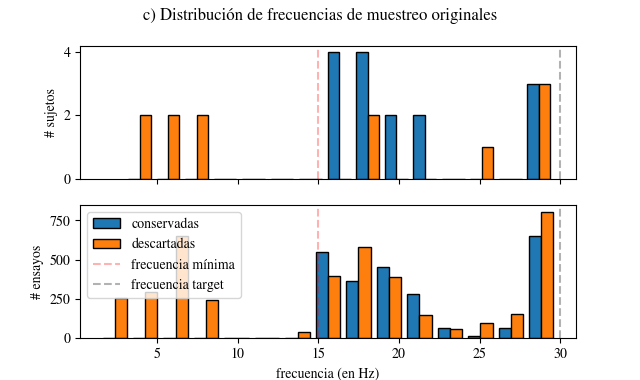
\includegraphics[width=0.7\linewidth]{img/second-sampling-frequencies-distribution.png}
  \end{figure}

\end{frame}

\begin{frame}{Anchos de pantalla}

  TODO: Acomodar subplots y mostrarlo solo por estimaciones para que sea menos
  lío
  \begin{figure}
    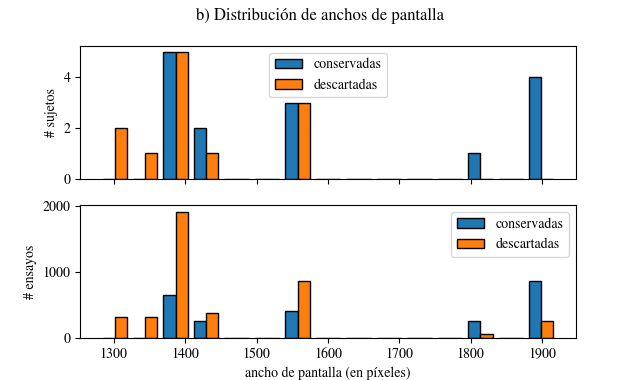
\includegraphics[width=0.7\linewidth]{img/second-widths-distribution.png}
  \end{figure}

\end{frame}

\begin{frame}{Estimaciones desviadas}

  TODO: Acomodar subplots
  \begin{figure}
    \includegraphics[width=0.8\linewidth]{img/skewed-estimations-examples.png}
  \end{figure}

\end{frame}

\subsection{Limpieza y normalización}

\subsection{Detección de sacadas}

\begin{frame}{~}

  Luego de normalizar, se considerará un intervalo como una sacada si:
  \begin{enumerate}
    \item La mirada se mueve en una misma dirección
    \item El intervalo dura al menos 40 ms
    \item Se recorre \textit{cierta} distancia mínima durante ese intervalo
    \item El desplazamiento es lo \textit{suficientemente rápido}
  \end{enumerate}
  Implementación \textit{ad hoc} cuya calidad no fue estudiada.

\end{frame}

\subsection{Conclusiones generales replicadas}

\begin{frame}{~}
  \begin{columns}
    \begin{column}{0.5\textwidth}
      \begin{figure}
        \centering
        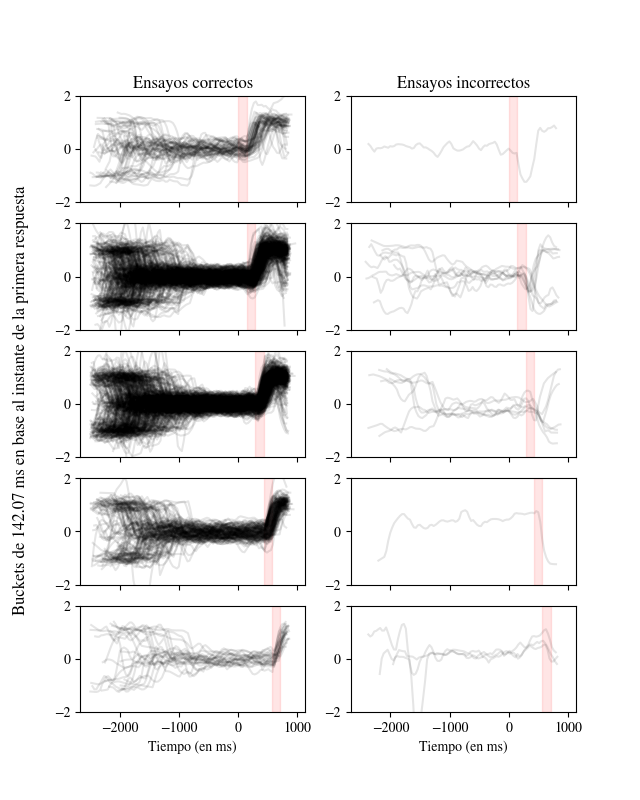
\includegraphics[width=\linewidth]{img/second-disaggregated-prosaccades.png}
      \end{figure}
    \end{column}
    \begin{column}{0.5\textwidth}
      \begin{figure}
        \centering
        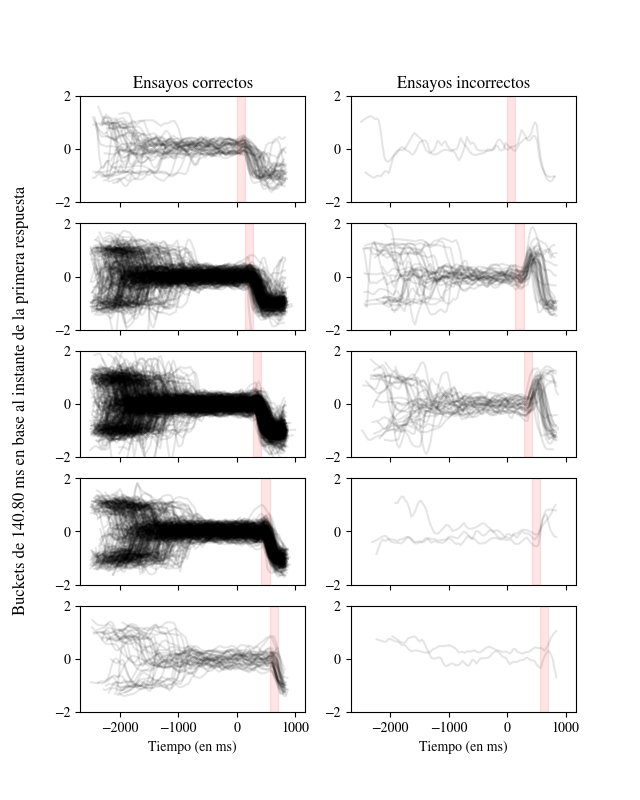
\includegraphics[width=\linewidth]{img/second-disaggregated-antisaccades.png}
      \end{figure}
    \end{column}
  \end{columns}
\end{frame}

\subsection{Grupos etarios no representados}

\begin{frame}{~}
  TODO: Cambiarlo para que sólo muestre los sujetos y no los ensayos
  \begin{columns}
    \begin{column}{0.5\textwidth}
  \begin{figure}
    \centering
    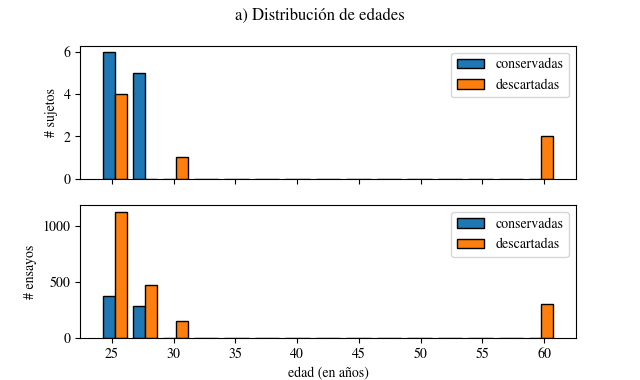
\includegraphics[width=\linewidth]{img/first-ages-distribution.png}
    \caption{Primera instancia}
  \end{figure}
      
    \end{column}
    \begin{column}{0.5\textwidth}
  \begin{figure}
    \centering
    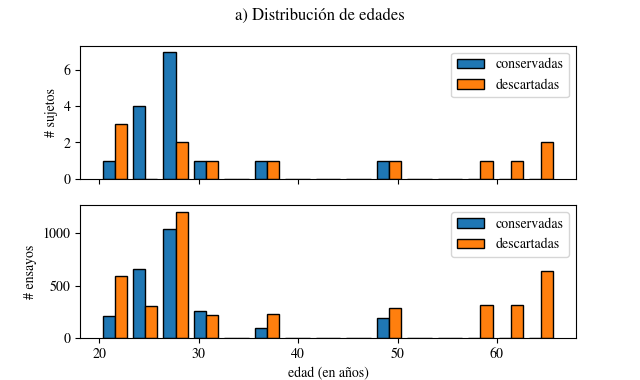
\includegraphics[width=\linewidth]{img/second-ages-distribution.png}
    \caption{Segunda instancia}
  \end{figure}
    \end{column}
  \end{columns}
\end{frame}

\subsection{Menos datos de lo esperado}



\section{Conclusiones}

\begin{frame}{~}
  \begin{itemize}
    \item Se obtuvo un prototipo de \textit{eye tracker} para navegadores web
    \item Potencial para realizar análisis clínicos remotos
    \item Campo aún en sus primeros pasos
    \item Precisión muy por debajo de aquella alcanzable por \textit{eye
      trackers} profesionales
  \end{itemize}
\end{frame}

\subsection{Limitaciones}

\begin{frame}{Implementativas}
  TODO: Las limitaciones y trabajo futuro no ponerlas todas y en cambio referir
  a la tesis \par

. bajas frecuencias
. pestañeos
. estimación del tamaño de la pantalla
. imprecisión en la duración de cada frame, problemático si se quiere mostrar
  un estímulo durante una corta duración de tiempo

  \begin{figure}
    \centering
    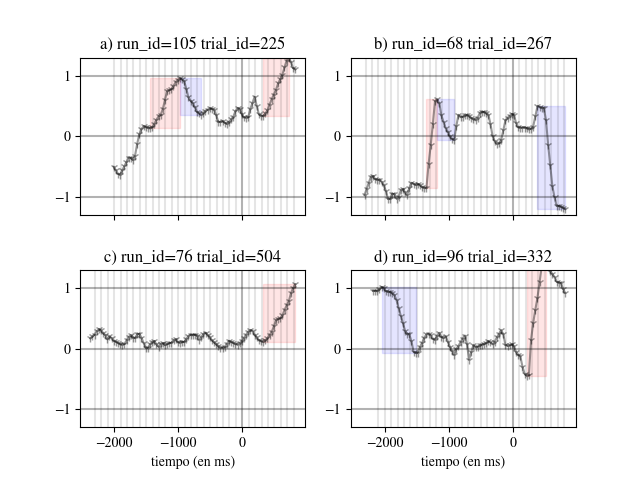
\includegraphics[width=0.9\linewidth]{img/undetected-saccades-examples.png}
    \caption{Ejemplos de sacadas no detectadas}
  \end{figure}
\end{frame}

\begin{frame}{Experimentales}
. proporción de datos filtrados demasiado elevada
. necesidad de revisar la causa de las altas tasas de correctitud obtenidas
. representatividad de distintos grupos etarios
\end{frame}

\subsection{Trabajo futuro}

\begin{frame}{Análisis de datos}
. Investigar e implementar mecanismos estándares de detección de sacadas, lo
  cual podría basarse en la previa construcción de un dataset etiquetado de
  sacadas
. Revisar criterios de exclusión para asegurarse de no estar filtrando datos
  válidos
. Realizar nuevas rondas de experimentación, estimando previamente la cantidad
  de ensayos necesarios para asegurar cantidades suficientes en los grupos
  incorrectos y en los distintos grupos etarios
\end{frame}

\begin{frame}{Análisis de sensibilidad}
. propuesta sobre experimento para recolectar datos y establecer métricas de
  calidad sobre las estimaciones obtenidas por la herramienta
TODO: Acá combinar un poco lo que quedó en la tesis y lo que pensé para
      sensitivity analysis
\end{frame}

\begin{frame}{Prototipo desarrollado}
. optimizar frecuencia de muestreo
. reexplorar detección de descalibraciones y qué significa que el sistema esté
  descalibrado
. mejorar la calibración, generalizarla a más puntos de interés
. detección de pestañeos
. estimación del tamaño de la pantalla y posibilidad de mostrar estímulos en
  grados
. verificación de condiciones iniciales
TODO: Extender con lo que haya escrito en la tesis
\end{frame}

\begin{frame}{\textit{Eye tracking} en navegadores \textit{web}}
. extender bibliografía que aplique a nuestro contexto
. eye tracking web no podría atacar algunos problemas que sí puede el eye
  tracking tradicional, pero al ser remoto y de bajo costo es posible que
  permita atacar nuevos problemas. Deben entonces buscarse tales problemas
\end{frame}

\end{document}


\chapter{Desarrollo}

\documentclass[aspectratio=169]{beamer}

\usepackage{subcaption}
\usepackage{emoji}

\title{Evaluación y desarrollo de \textit{eye tracking} remoto en navegadores
\textit{web}}
\author{Francisco Figari, Juan Kamienkowski, Gustavo Juantorena, Bruno Bianchi}
\date{Buenos Aires, 2022}
\titlegraphic{
\includegraphics[width=8em]{img/logo-fcen.png}}

\setbeamertemplate{navigation symbols}{}

% TODO: Hacer que esto sea opcional
\setbeamertemplate{frametitle}{
  \insertsectionhead\par
  \vspace*{0.2mm}
  \insertsubsectionhead\par
  \vspace*{0.2mm}
  \insertframetitle
}

\begin{document}

\frame{\titlepage}

\section{Implementación}

\begin{frame}{\texttt{WebGazer} como punto de partida}

  \begin{columns}
    \begin{column}{.5\textwidth}
      \begin{itemize}
        \item[\emoji{thumbs-up}] Extracción de frames a través de la API del
          navegador
        \item[\emoji{thumbs-up}] Modelos de localización de los ojos y de
          estimación de la mirada
        \item[\emoji{thumbs-down}] Calibración inadecuada
        \item[\emoji{thumbs-down}] Ausencia de notificación de descalibraciones
        \item[\emoji{party-popper}] Corrregida falla de \texttt{WebGazer} que
          causaba \textit{crashes} del navegador en ciertas notebooks
      \end{itemize}
    \end{column}

    \begin{column}{.5\textwidth}
      \begin{figure}
        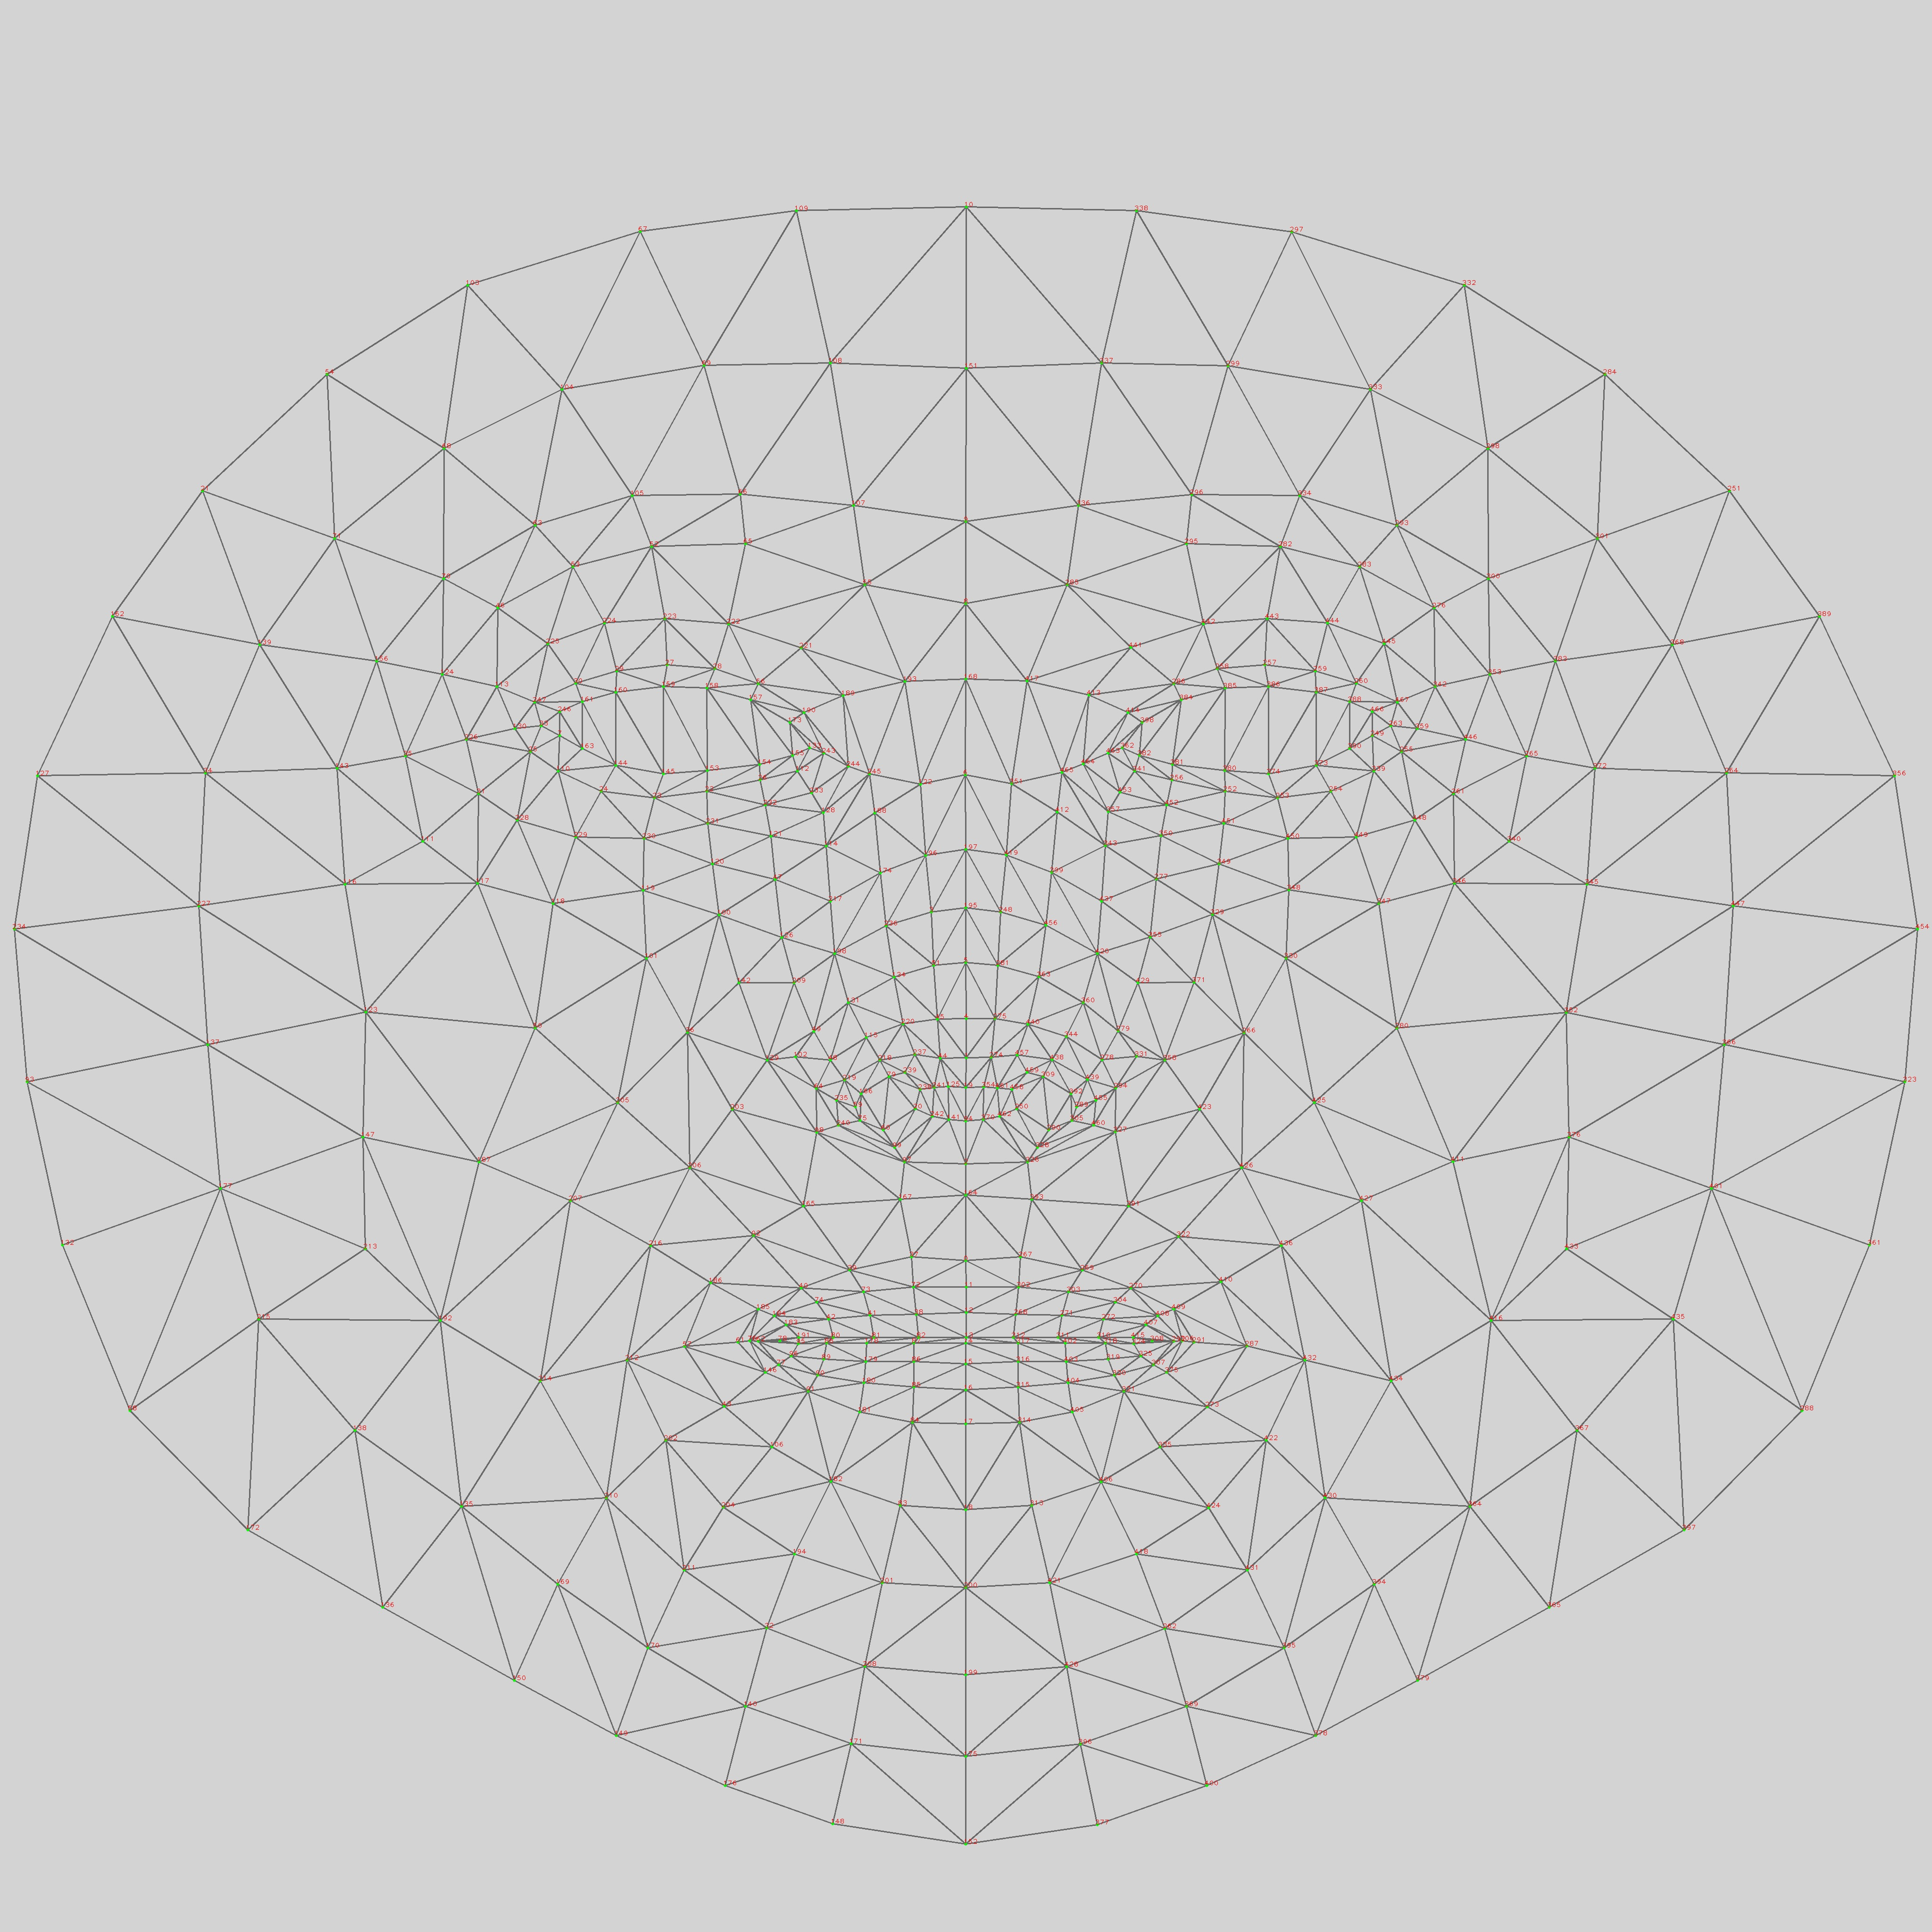
\includegraphics[width=0.75\linewidth]{img/facemesh-kepyoints.jpg}
        \caption{\textit{Output} del modelo de \textit{facemesh} utilizado por
        \texttt{WebGazer} para la localización de los ojos}
      \end{figure}
    \end{column}
  \end{columns}

\end{frame}

\begin{frame}{Calibración y validación}
  \begin{itemize}
    \item Nuestro caso de uso no garantiza interacciones

    \item Se muestran una serie de puntos, para cada uno de los cuales el
      usuario tendrá que fijar la mirada y presionar la barra de espacio
    
    \item Validación post calibración implementada de similar manera

    \item[\emoji{party-popper}] \texttt{WebGazer} adaptado para evitar cómputos
      ya no necesarios
  \end{itemize}
\end{frame}

\begin{frame}{Notificación de descalibración}

  \begin{columns}
    \begin{column}{.5\textwidth}
      \begin{itemize}
        \item Basada en detectar movimiento
        \item Instanciada luego de cada calibración
        \item Verificación realizada para cada \textit{frame}
        \item \emoji{party-popper} \texttt{WebGazer} adaptado para exponer los
          recuadros calculados en cada \textit{frame} por la rutina de
          localización de ojos
      \end{itemize}
    \end{column}

    \begin{column}{.5\textwidth}
      \begin{figure}
        \centering
        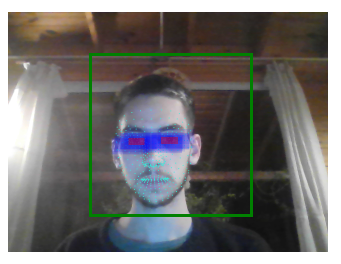
\includegraphics[width=\textwidth]{img/eyetracker-playground-screenshot.png}
        \caption{Detección de movimiento en funcionamiento}
      \end{figure}
    \end{column}
  \end{columns}

\end{frame}

\section{Experimentación}

\begin{frame}{Caso de estudio: tarea de antisacadas}

  \begin{columns}
    \begin{column}{.5\textwidth}
      \begin{itemize}
        \item Clínicamente relevante
        \item Resultados esperados ya establecidos
        \item Tarea simple para validar movimientos oculares
      \end{itemize}
    \end{column}
    \begin{column}{.5\textwidth}
      \begin{figure}
        \centering
        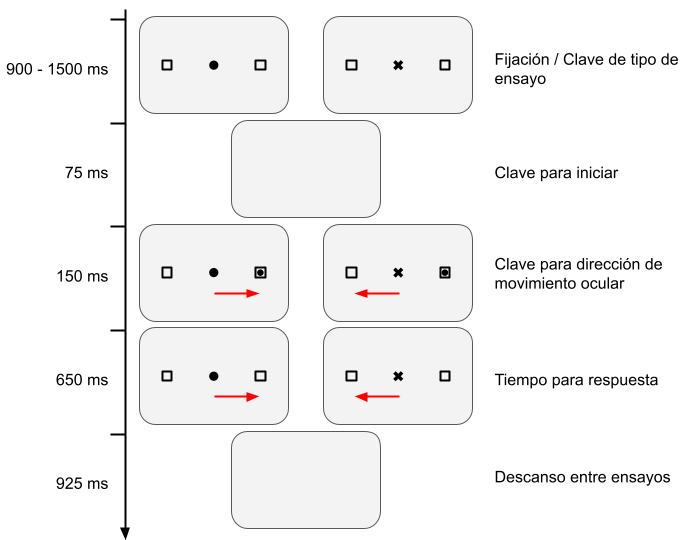
\includegraphics[width=\linewidth]{img/antisaccades-protocol.png}
        \caption{Protocolo de las tareas}
      \end{figure}
    \end{column}
  \end{columns}

\end{frame}

\begin{frame}{Primera instancia}
  \begin{itemize}
    \item Limitados a 10 minutos debido a una falla de \texttt{WebGazer}
    \item Únicamente ensayos de antisacada
    \item Recalibración luego de cada notificación de descalibración
    \item Sin validación post calibración
  \end{itemize}
\end{frame}

\begin{frame}{Segunda instancia}
  \begin{itemize}
    \item Duración superior a 20 minutos
    \item Ensayos de prosacadas y de antisacadas
    \item Recalibración cada 10 ensayos y sólo si se detectó una
      descalibración
    \item Con validación post calibración
  \end{itemize}
\end{frame}

\begin{frame}{Implementación y distribución}

  \begin{columns}
    \begin{column}{0.4\textwidth}
      \begin{figure}
        \centering
        
\includegraphics[width=\textwidth]{img/jspsych-logo.jpg}
      \end{figure}
    \end{column}
    \begin{column}{0.6\textwidth}
      \begin{figure}
        \centering
        
\includegraphics[width=0.8\textwidth]{img/cognition-run-logo.png}
        
\includegraphics[width=\textwidth]{img/neuropruebas-logo.jpg}
      \end{figure}
    \end{column}
  \end{columns}
\end{frame}


\section{Resultados}

\begin{frame}{Ejemplo de \textit{output} del sistema}
  \begin{figure}
    \centering
    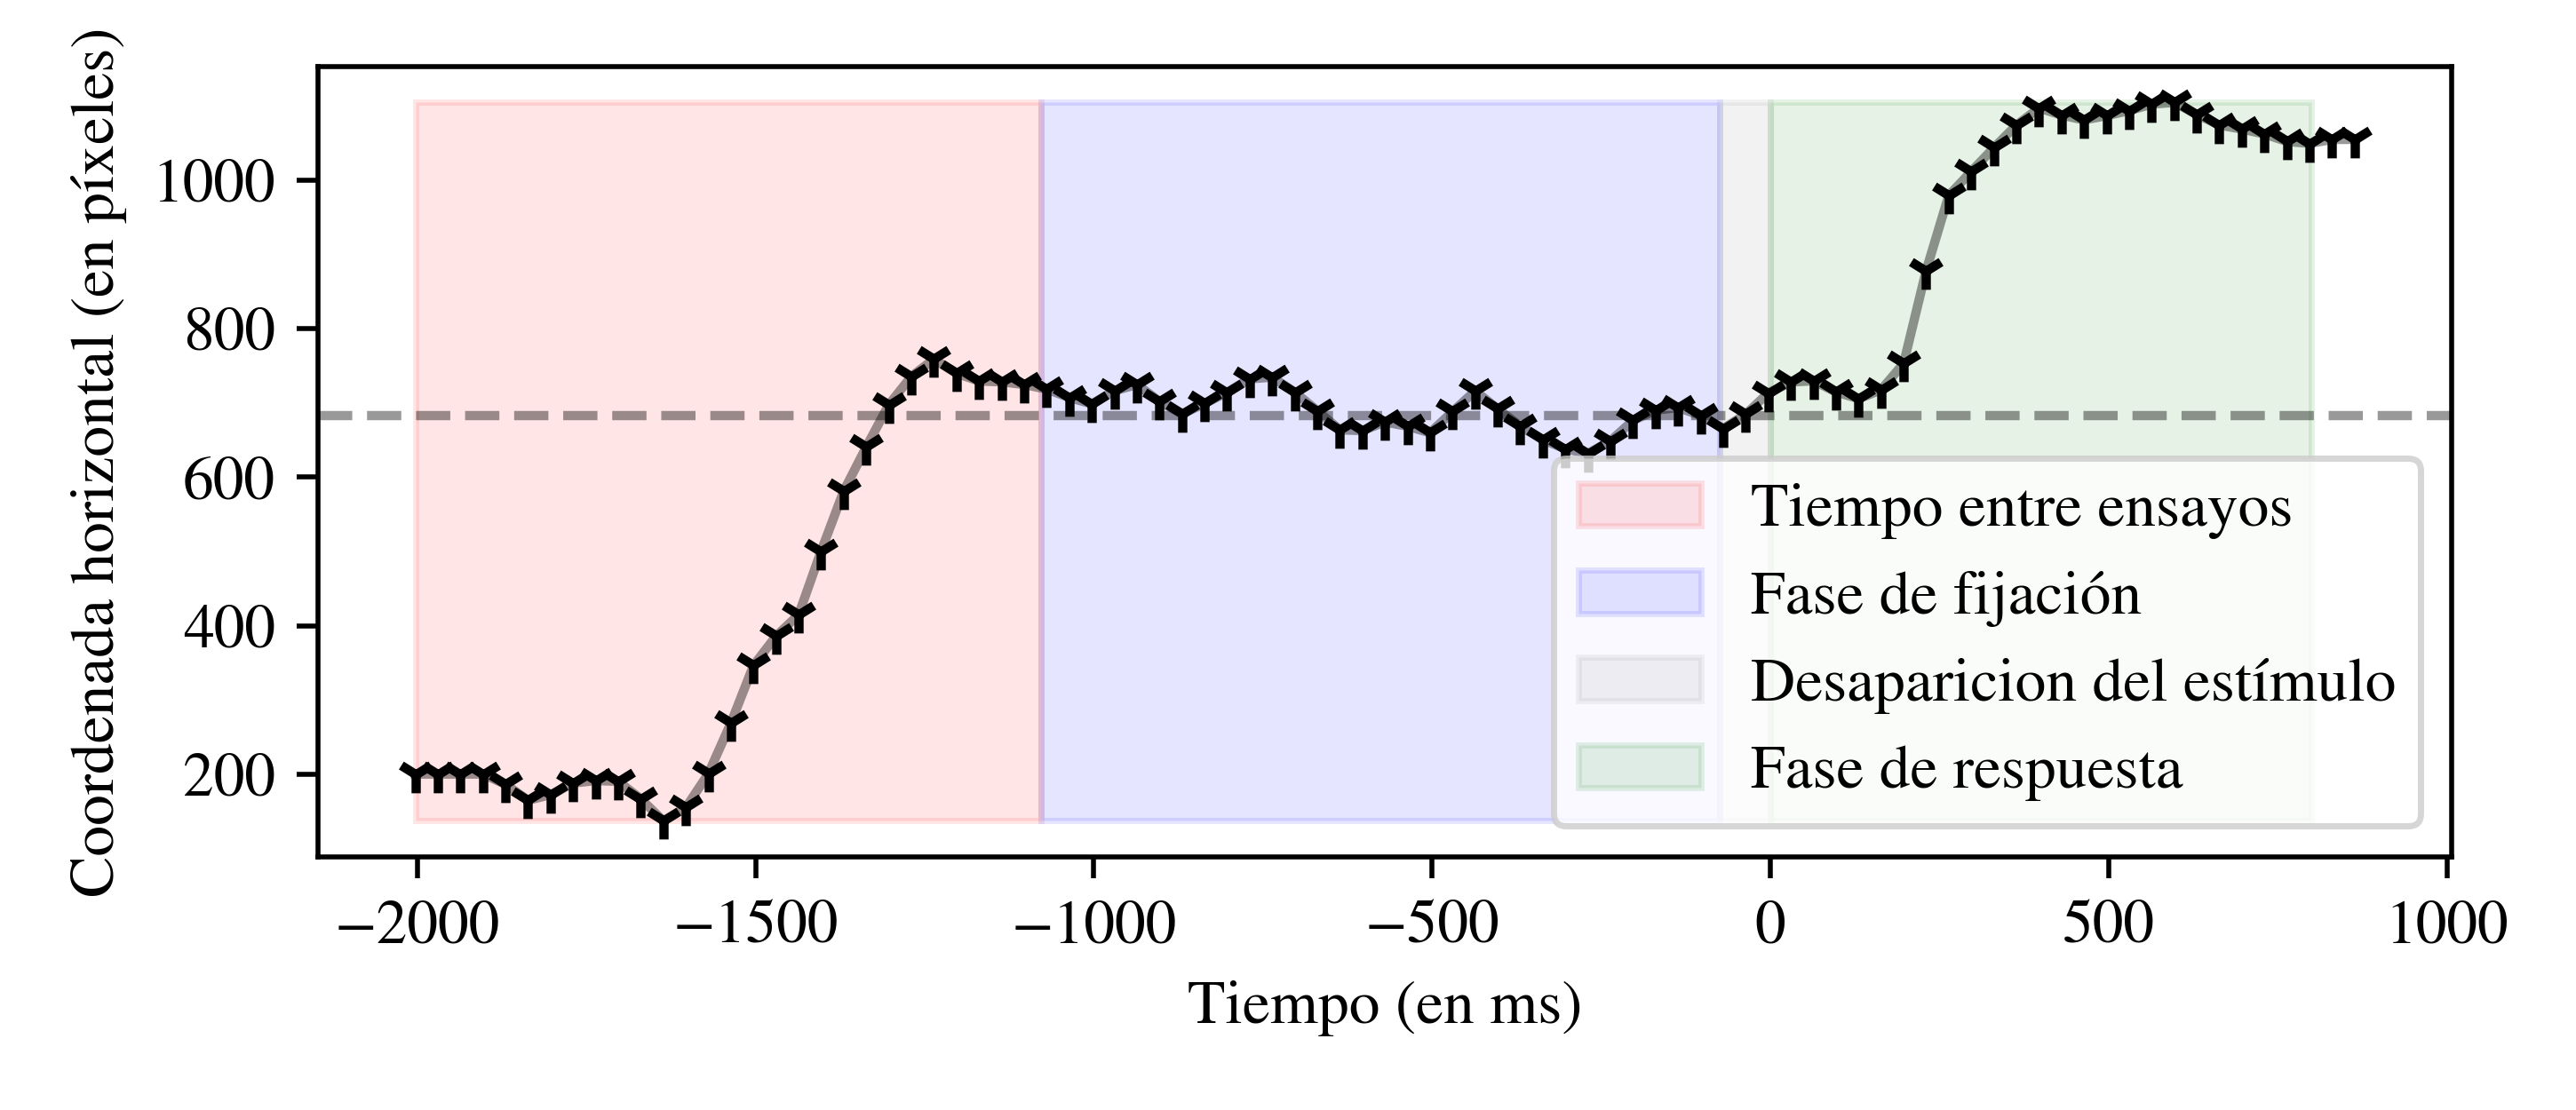
\includegraphics[width=\linewidth]{plots/output-example.png}
  \end{figure}
\end{frame}

\begin{frame}{Frecuencias de muestreo}
  \begin{figure}
    \centering
    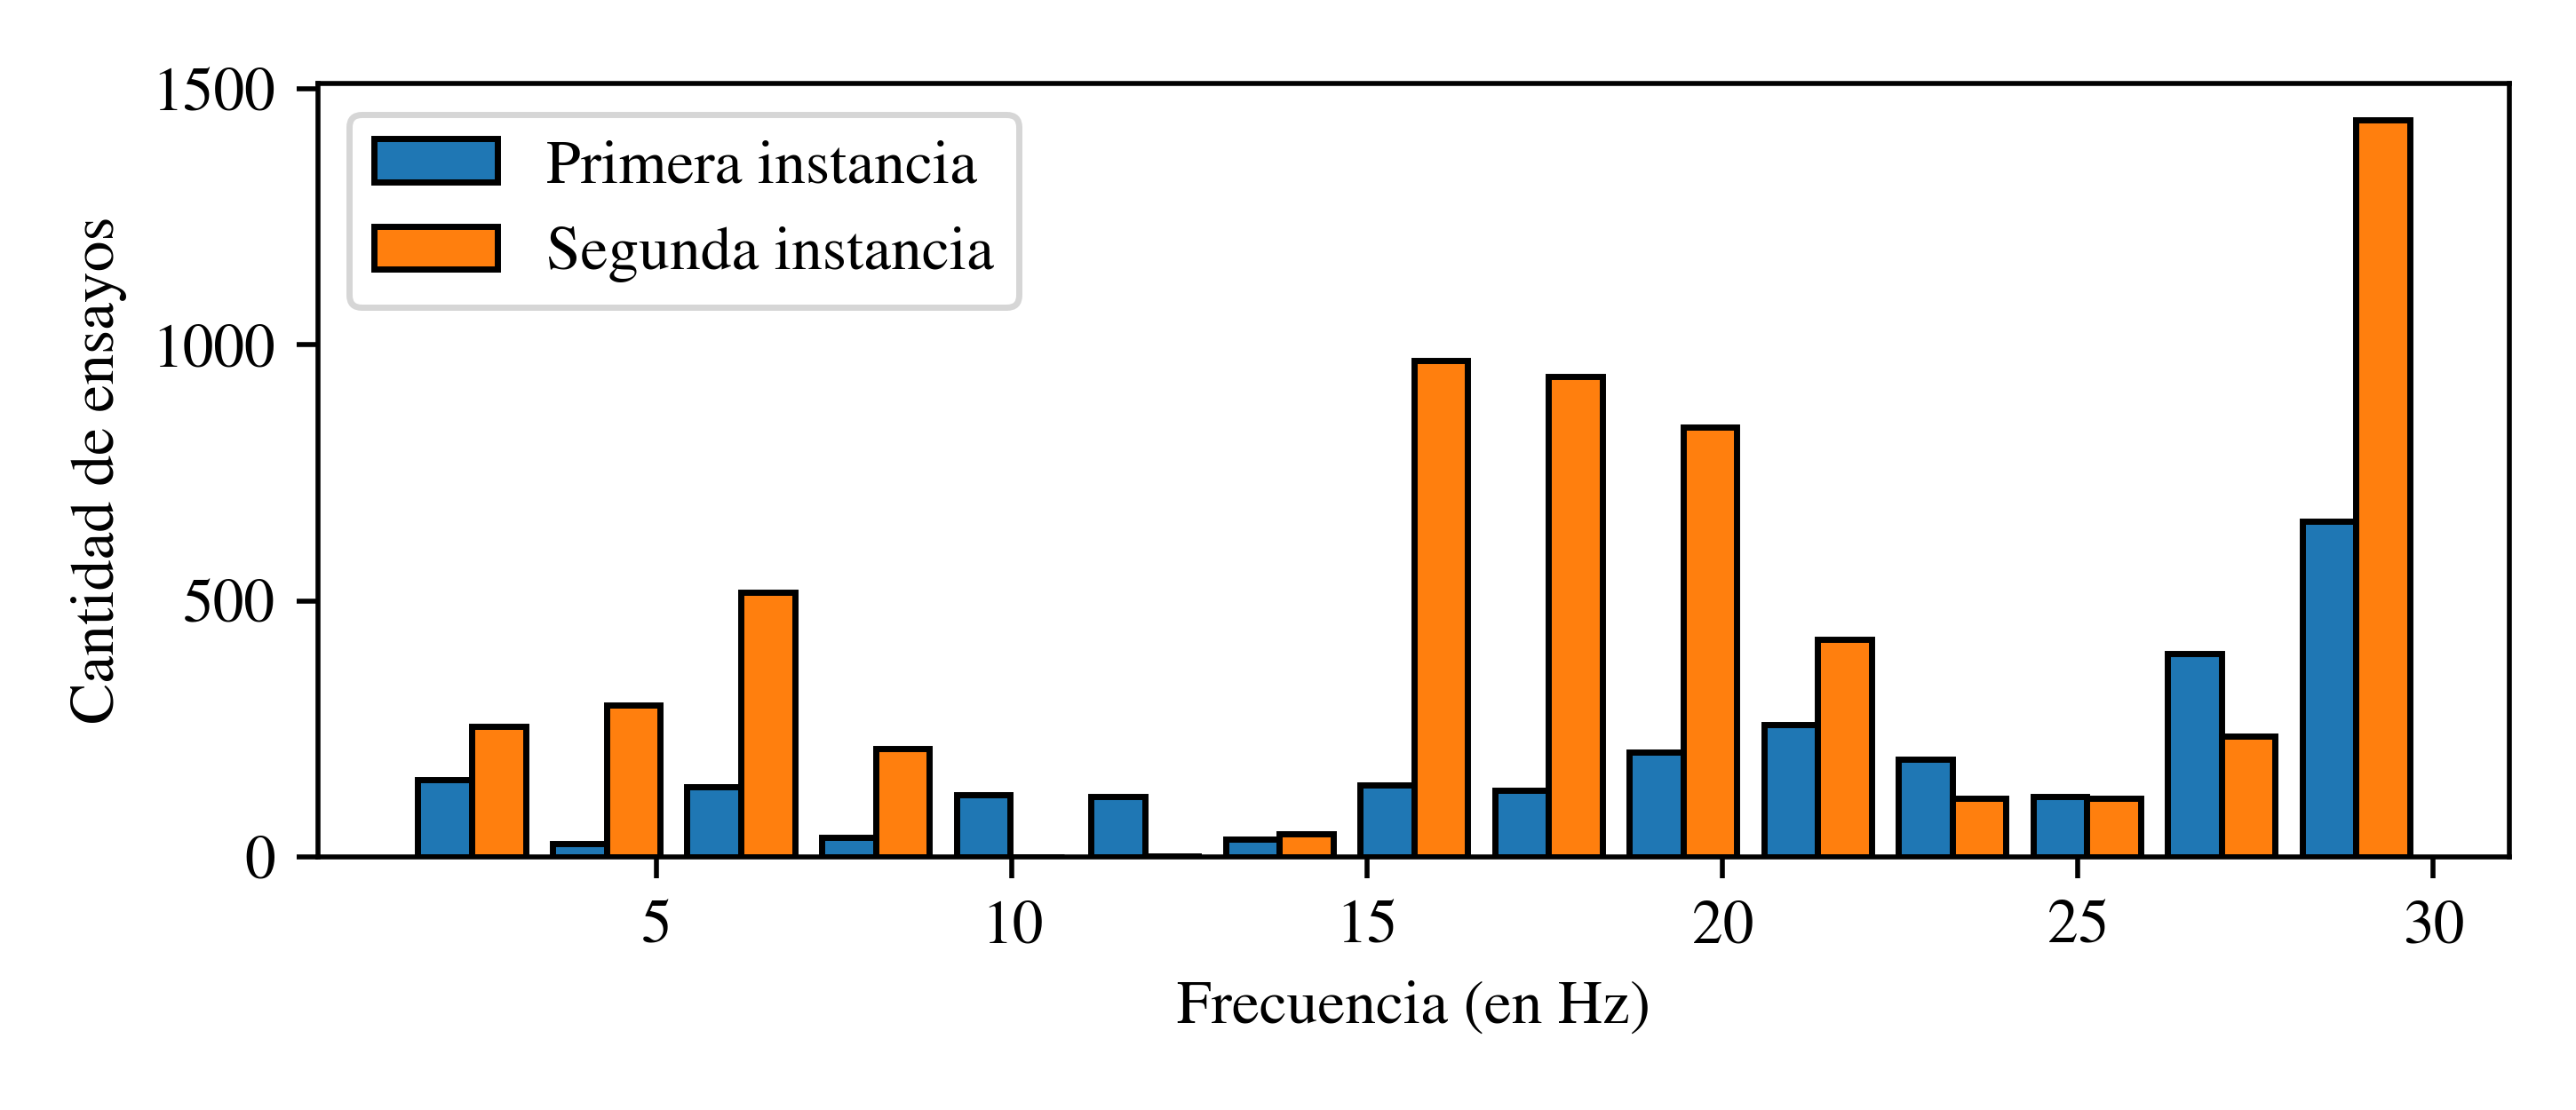
\includegraphics[width=\linewidth]{plots/sampling-frequencies-distribution.png}
  \end{figure}
\end{frame}

\begin{frame}{Anchos de pantalla}
  \begin{figure}
    \centering
    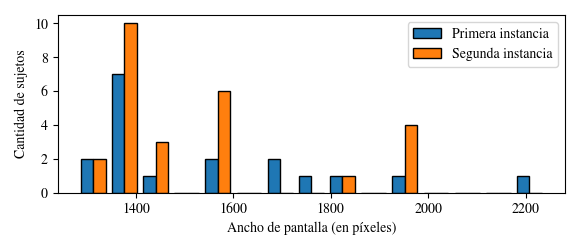
\includegraphics[width=\linewidth]{plots/screens-widths-distribution.png}
  \end{figure}
\end{frame}

\begin{frame}{Estimaciones desviadas}
  \begin{figure}
    \centering
    \includegraphics[width=\linewidth]{plots/skewed-estimations-examples.png}
    \caption{Las estimaciones de algunos sujetos están desviadas de los valores reales}
  \end{figure}
\end{frame}

\begin{frame}{Limpieza y normalización}
  \begin{columns}
    \begin{column}{0.4\textwidth}
      \begin{itemize}
        \item Ensayos descartados: \begin{itemize}
          \item frecuencia menor a 15 Hz
          \item a mano
          \item si el sujeto se distrajo de la tarea
        \end{itemize}
        \item Frecuencia de muestreo: \textit{Upsampling} a 30 Hz usando
          interpolación lineal
      \end{itemize}
    \end{column}
    \begin{column}{0.6\textwidth}
      \begin{figure}
        \centering
        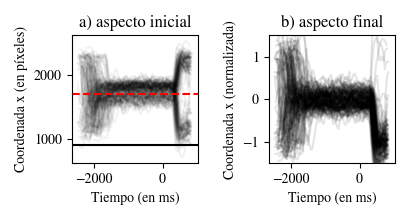
\includegraphics[width=\linewidth]{plots/normalization-example.png}
        \caption{Normalizado y espejado}
      \end{figure}
    \end{column}
  \end{columns}
\end{frame}

\begin{frame}{Detección de sacadas}
  \begin{columns}
    \begin{column}{0.5\textwidth}
      \begin{figure}
        \centering
        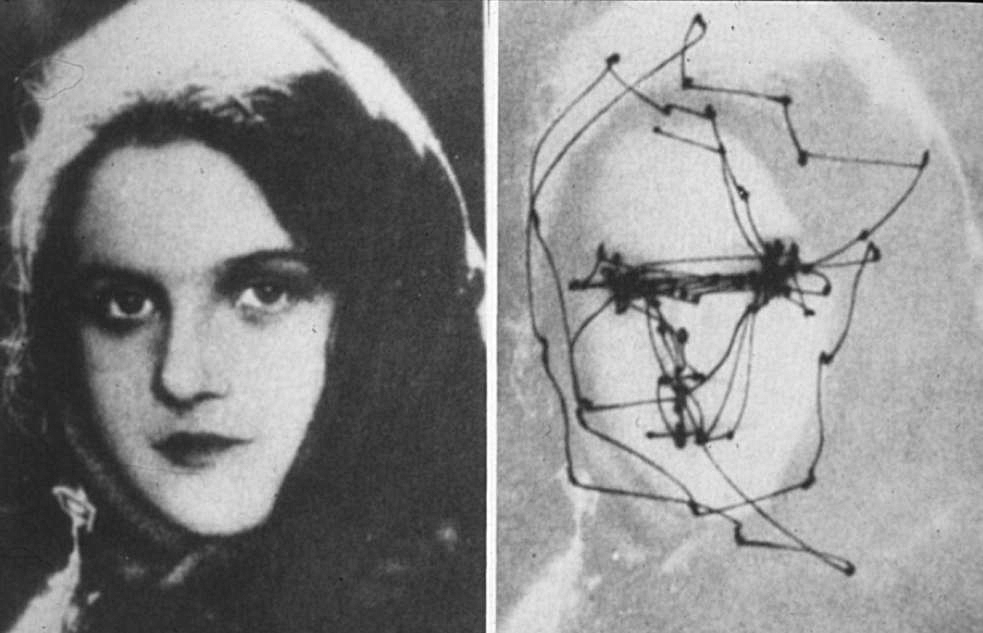
\includegraphics[width=\linewidth]{img/saccades-example.jpg}
        \caption{Los movimientos oculares muestran qué elementos de una imagen
        capturan la atención}
      \end{figure}
    \end{column}
    \begin{column}{0.5\textwidth}
      \begin{figure}
        \centering
        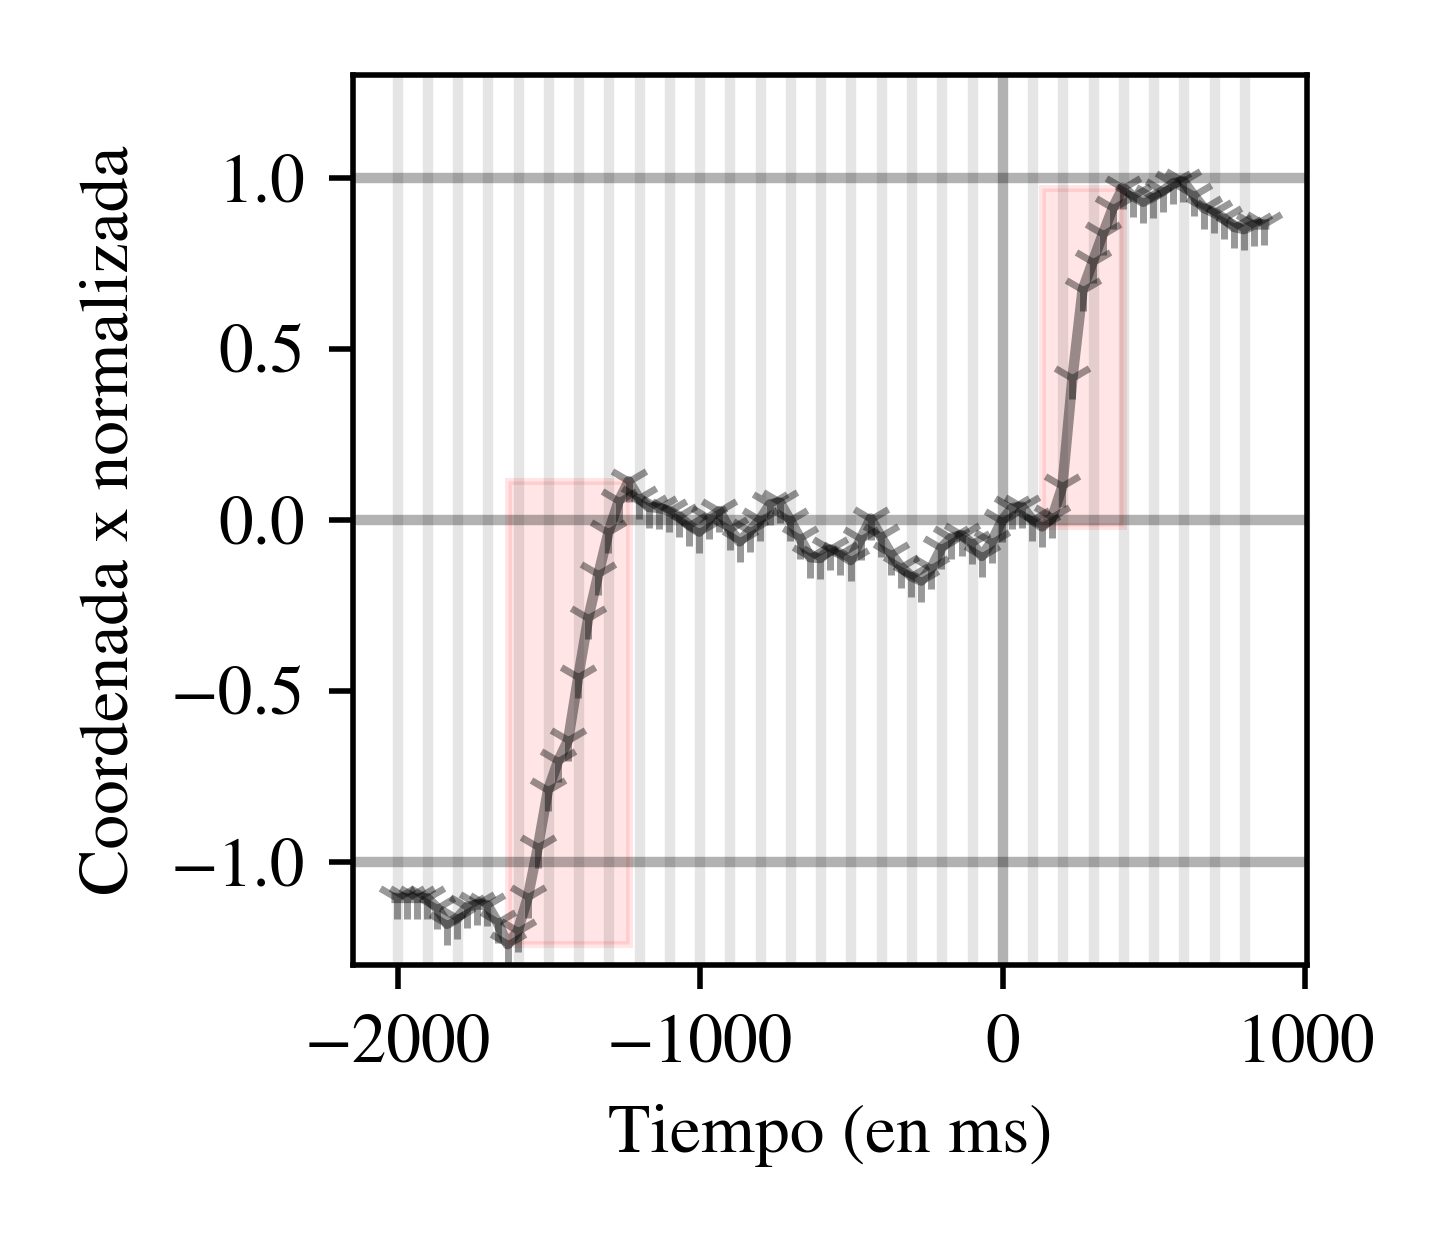
\includegraphics[width=\linewidth]{plots/detected-saccades-example.png}
        \caption{Sacadas detectadas sobre las estimaciones de un ensayo}
      \end{figure}
    \end{column}
  \end{columns}
\end{frame}

\begin{frame}{Conclusiones generales replicadas}
  \begin{table}
    \centering
    \begin{tabular}{ l | c | c | c }
      & correctitud & \multicolumn{2}{ c }{tiempo de respuesta (ms)} \\
      &             & correcto & incorrecto \\
      \hline
      antisacada & 81.29\% & 509 (93) & 346 (105) \\
    \end{tabular}
    \caption{Primera instancia}
  \end{table}
  
  \begin{table}
    \centering
    \begin{tabular}{ l | c | c | c }
      & correctitud & \multicolumn{2}{ c }{tiempo de respuesta (ms)} \\
      &             & correcto & incorrecto \\
      \hline
      antisacada & 94.82\% & 358 (109) & 299 (103) \\
      \hline
      prosacada & 98.09\% & 320 (108) & 311 (150) \\
    \end{tabular}
    \caption{Segunda instancia}
  \end{table}

  % TODO: Poner marker negativo acá
  En la bibliografía para la tarea de antisacadas se reportan \textbf{valores
  de correctitud} más cercanos al rango $[60\%, 75\%]$.
\end{frame}

\begin{frame}{Menos datos de lo esperado}
  \begin{columns}
    \begin{column}{0.4\textwidth}
      \begin{itemize}
        \item Cantidad de ensayos iniciales baja en relación a otros trabajos
        \item Descarte de aproximadamente $\frac{2}{3}$ de los datos
        \item Altas e inesperadas tasas de correctitud
      \end{itemize}
    \end{column}

    \begin{column}{0.6\textwidth}
      \begin{table}
        \centering

        \begin{tabular}{ l | c | c }
          Antisacadas   & incorrecto  & correcto \\
          \hline
          \# total      & 64          & 1173 \\
          \hline
          \# por sujeto & 4.57 (2.84) & 78.20 (40.38)
        \end{tabular}

        \vspace{0.3cm}

        \begin{tabular}{ l | c | c }
          Prosacadas    & incorrecto  & correcto \\
          \hline
          \# total      & 22          & 1134 \\
          \hline
          \# por sujeto & 2.44 (1.23) & 75.59 (38.58)
        \end{tabular}

        \caption{Desbalance entre grupos incorrecto y grupo correcto}
      \end{table}
    \end{column}
  \end{columns}
\end{frame}

\begin{frame}{~}
  fin
\end{frame}

\section{Motivación}

\begin{frame}{~}

  \begin{itemize}
      \item Los ojos como entrada a los procesos cognitivos y estados
        emocionales de una persona
      \item Frecuentemente estudiados en el contexto de la neuropsicología
        digital para estimar el comportamiento
      \item Importante incluso cuando no son el foco del análisis
        (\textit{e.g.}, detección de caras)
      % utilizado también en el desarollo HMI, en el estudio de usabilidad de
      % interfaces, recientemente en el campo de la oftalmología para estimar
      % el campo visual
      \item Usos en otras disciplinas
  \end{itemize}

  \begin{figure}
    \begin{subfigure}{0.49\textwidth}
      \centering
      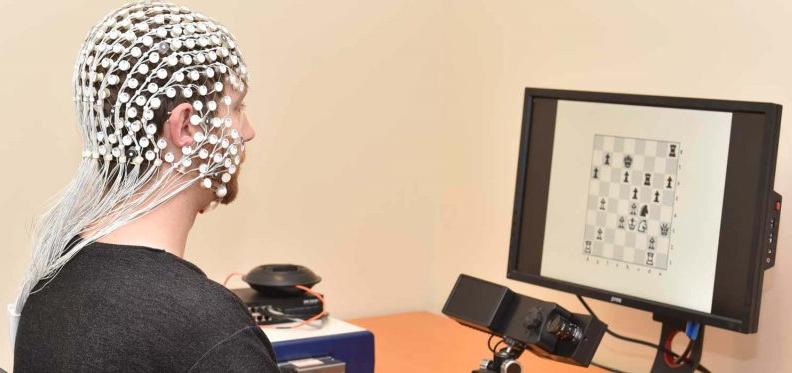
\includegraphics[width=\linewidth]{img/eye-link-eeg.jpg}
      \caption{\textit{Eye tracking} combinado con electroencefalograma}
    \end{subfigure}
    \begin{subfigure}{0.49\textwidth}
      \centering
      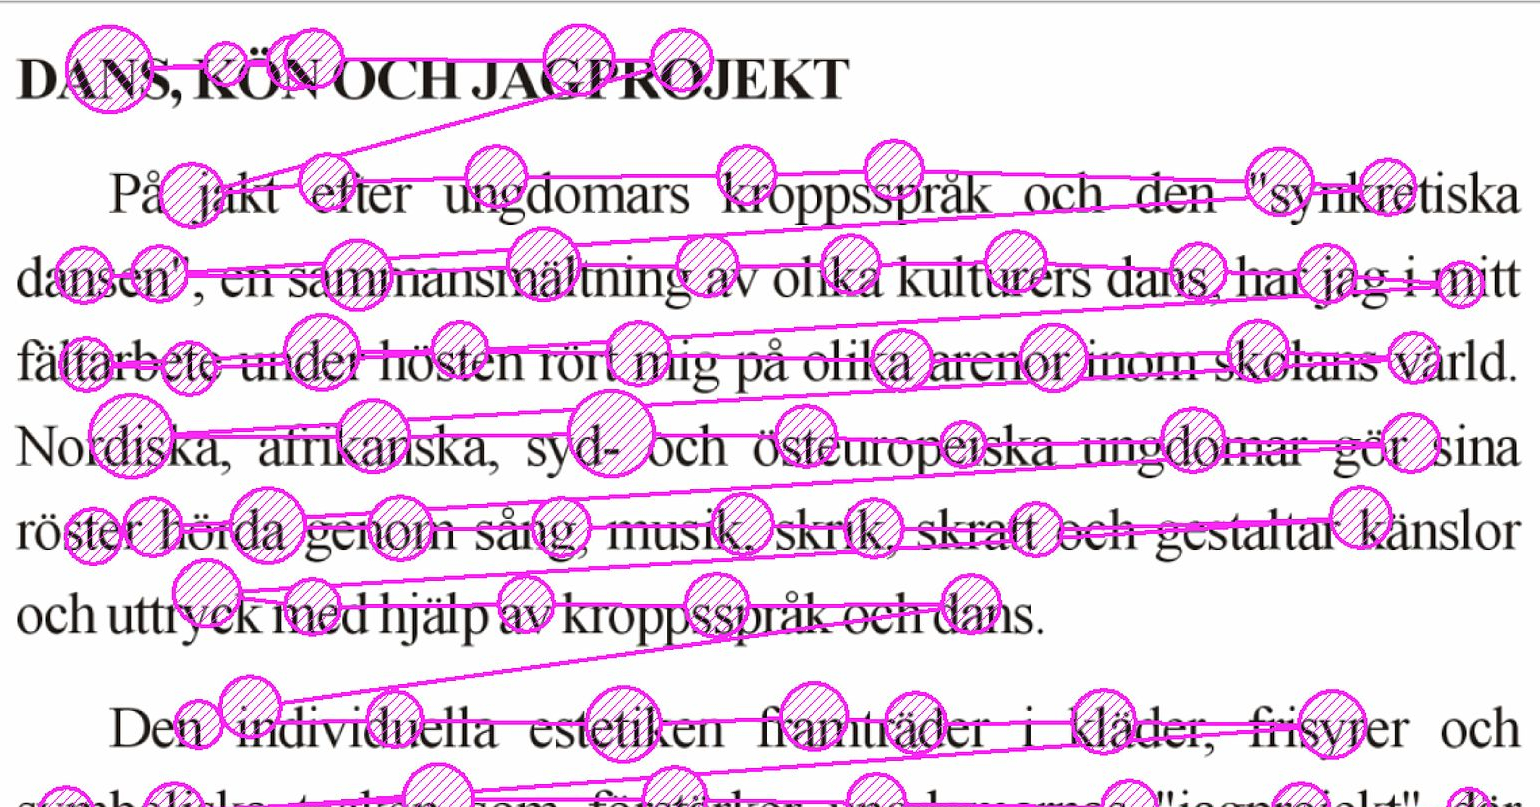
\includegraphics[width=\linewidth]{img/reading-fixations-saccades.jpg}
      \caption{Estimación de la mirada durante una tarea de lectura}
    \end{subfigure}
  \end{figure}

\end{frame}

\begin{frame}{~}

  \begin{itemize}
    \item Comunmente resuelto con sistemas comerciales cerrados
    \item Costos altos (entre 5000 y 40000 euros) mientras que el hardware en
      sí representa una pequeña fracción de estos (entre 200 y 600 euros)

    % si falta algún dato (e.g., la precisión del diámetro de la pupila) no
    % se lo puede saber
    \item Imposibilidad de auditar la implementación
    \item Necesidad de asistir a un laboratorio
  \end{itemize}

  \begin{figure}
    \begin{subfigure}{0.49\textwidth}
      \centering
      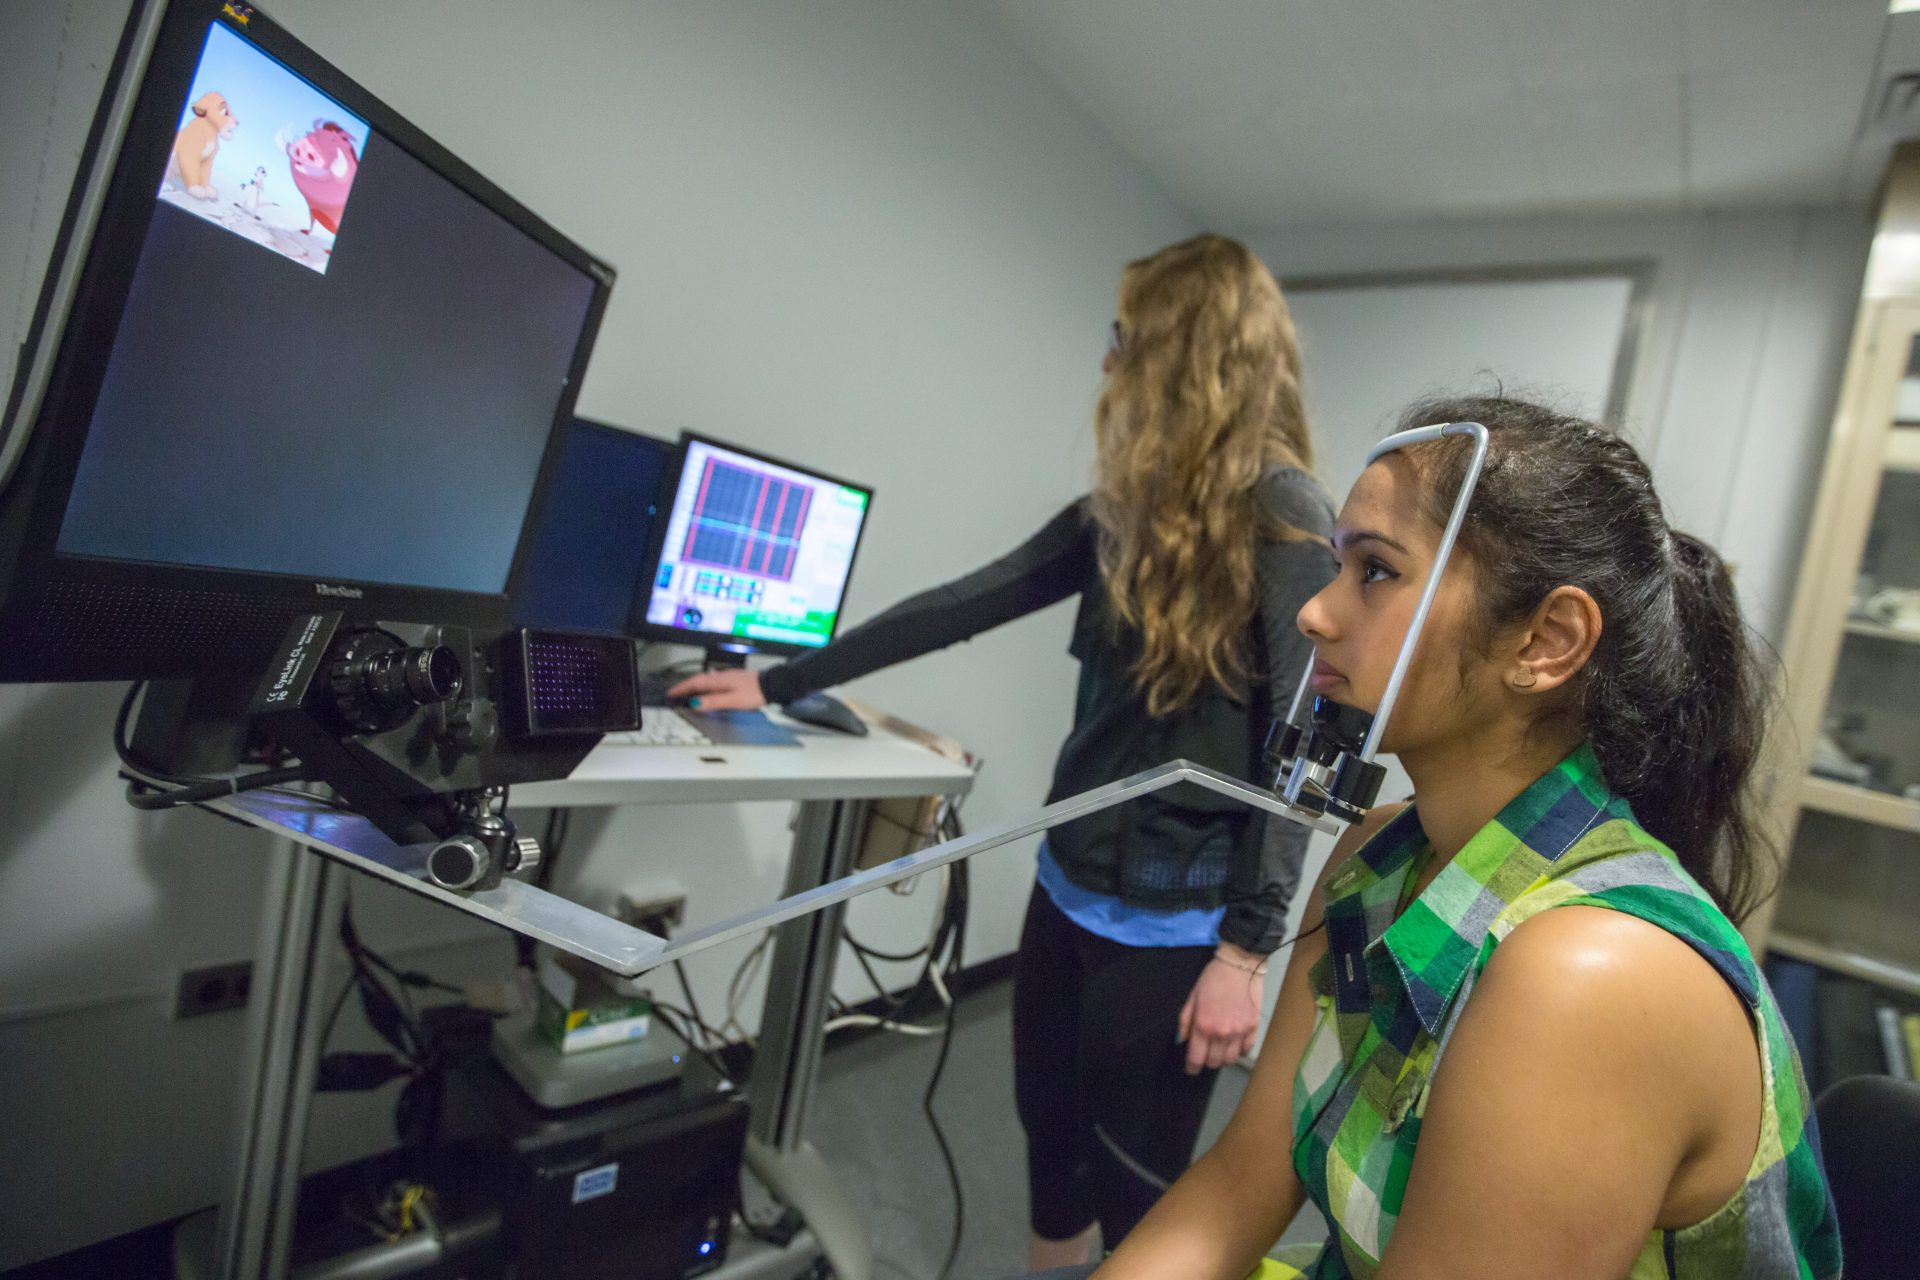
\includegraphics[width=0.6\linewidth]{img/eye-link-chinrest.jpg}
      \caption{La reestricción de movimiento facilita mantener calibrado el
      sistema}
    \end{subfigure}
    \begin{subfigure}{0.49\textwidth}
      \centering
      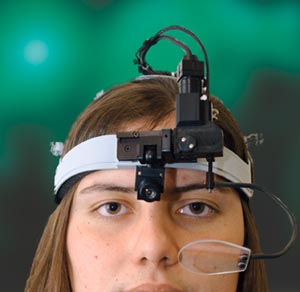
\includegraphics[width=0.5\linewidth]{img/eye-tracker-head-mounted.jpg}
      \caption{\textit{Eye tracker} montado a la cabeza}
    \end{subfigure}
  \end{figure}

\end{frame}

\begin{frame}{~}

  \begin{columns}
    \begin{column}{0.4\textwidth}
      \begin{itemize}
        \item Interés en proveer software de \textit{eye tracking}

        \item Posibilidad de \textit{crowdsourcing}

          % e.g., detectar pérdidas de atención en clases masivas
        \item Potencial para nuevas aplicaciones
      \end{itemize}

    \end{column}
    \begin{column}{0.6\textwidth}

      \begin{figure}
        \begin{subfigure}{0.49\textwidth}
          \centering
          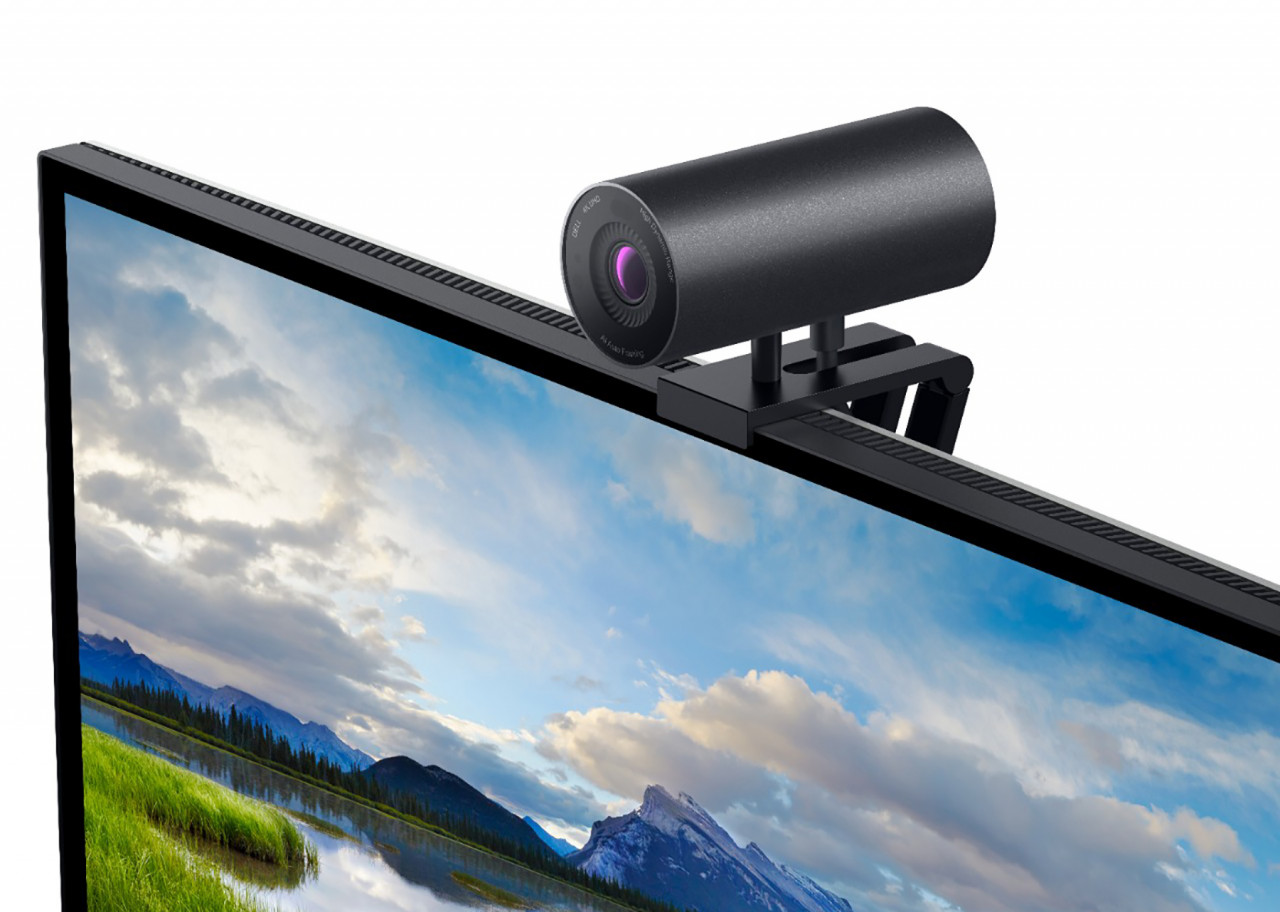
\includegraphics[width=0.8\linewidth]{img/external-webcam.jpg}
        \end{subfigure}
        \begin{subfigure}{0.49\textwidth}
          \centering
          \includegraphics[width=0.8\linewidth]{img/notebook.jpg}
        \end{subfigure}
        \caption{Webcams domésticas ya disponibles}
      \end{figure}

      \begin{figure}
        \begin{subfigure}{0.49\textwidth}
          \centering
          \includegraphics[width=0.6\linewidth]{img/basler-camera.jpg}
        \end{subfigure}
        \begin{subfigure}{0.49\textwidth}
          \centering
          \includegraphics[width=0.8\linewidth]{img/basler-cameras-with-lens.png}
        \end{subfigure}
        \caption{Hardware profesional adquirible por una fracción del costo}
      \end{figure}


    \end{column}
  \end{columns}
\end{frame}

\section{Objetivos}

\begin{frame}{~}

  \begin{itemize}
    \item Evaluar implementaciones recientes con similares motivaciones
    % - entender el problema
    % - definir los requerimientos
    % - establecer qué puede reutilizarse

    \item Implementar un prototipo de \textit{eye tracker} que corra en
      navegadores \textit{web} y que esté orientado a análisis clínicos
    % - adaptar lo que pudiera reutilizarse
    % - implementar los módulos que faltaran

    \item Emular análisis clínicos remotos y recolectar datos utilizando el
      prototipo implementado

    \item Establecer la capacidad del prototipo en replicar conclusiones
      establecidas con \textit{eye trackers} profesionales de laboratorio

  \end{itemize}

\end{frame}

\section{Desarmando el problema de \textit{eye tracking} web}

\begin{frame}{~}
  \begin{columns}
    \begin{column}{0.5\textwidth}
      \begin{itemize}
        \item Estimar qué coordenada de la pantalla está mirando el usuario en
          un contexto de estudios clínicos
        \item Un \textit{stream} de frames de la webcam como \textit{input}
        \item Se divide en \textbf{localizar los ojos} y luego \textbf{estimar
          la mirada}
        \item Calibraciones necesarias en cada sesión de uso
      \end{itemize}
    \end{column}
    \begin{column}{0.5\textwidth}
      \begin{figure}
        \centering
        TODO: Reemplazar esto por un único plot que ejemplifique el output
        deseado
        \includegraphics[width=\linewidth]{img/eye-tracking-output-example.png}
        \caption{Sacadas detectadas sobre serie de tiempo de la coordenada x}
      \end{figure}
    \end{column}
  \end{columns}
\end{frame}

\begin{frame}{~}
    \begin{itemize}
    \item Resultados consistentes dentro de una misma población
    % - mayor tasa de correctitud para los casos de prosacada que para aquellos de antisacada
    % - para los grupos correctos se esperan mayores tiempos de respuesta en las repeticiones de antisacadas que en aquellas de prosacadas
    % - a mayor edad menor rendimiento en la tarea, tanto en latencia como en correctitud

    \item Búsqueda de establecer resultados para poblaciones de distinta condición neuropsicológica
    % - ditintos tipos de lesiones cerebrales
    % - déficit de atención, esquizofrenia, síndrome de Parkinson, síndrome de Tourette
    % - individuos sanos, efectos de la edad

    \item Comparación dificultosa entre distintos trabajos
    % - se obtienen valores del mismo orden (RT y correctitud) para pacientes sanos en un estudio que para pacientes con esquizofrenia de otro estudio
    \end{itemize}

\end{frame}

\section{Alternativas al \textit{eye tracking} tradicional}

\subsection{Trabajos previos}

\begin{frame}{~}

  TODO: Separar esto en varios frames
  \begin{itemize}
    \item \texttt{PupilEXT}: software para realizar pupilometría; deben
      proveerse cámaras profesionales y emisores de luz infrarroja; TODO:
      imagen pupilometría

    % hay que resaltar la importancia de esto de analizar el momento de mayor
    % coincidencia
    \item \texttt{PACE}: aplicación de escritorio basada en webcam; calibran en
      base a interacciones del usuario; analizar el momento de mayor
      coincidencia entre la mirada y la posición de la interacción; TODO:
      alguna imagen del paper

    \item \texttt{TurkerGaze}: aplicación web basada en webcam; generación de
      mapas de saliencia a través de \textit{crowdsourcing}; TODO: imagen mapas
      de saliencia

    \item \texttt{WebGazer}: aplicación web basada en webcam; se basan en
      \texttt{PACE} y \texttt{TurkerGaze}; provisto en forma de paquete; TODO:
      screenshot del paquete

  \end{itemize}

\end{frame}

\subsection{Implicancias del contexto remoto de navegador \textit{web}}

\begin{frame}{~}

  \begin{itemize}
    \item[+] Posibilidad de reutilizar cámaras web

    \item[+] Compatibilidad con otras herramientas web, en particular
      \texttt{JSPsych}

    % no es el fin del mundo pero es un lenguaje bastante odiado e implica
    % dificultades en cuanto a la precisión. Por ejemplo, la duración de cada
    % frame va a ser variable, lo que dificulta mostrar estímulos durante
    % cortas cantidades de tiempo
    \item Necesidad de implementar sobre JavaScript

    % no sólo las webcams son variables si no que tmb la compu donde corre el 
    % programa
    \item[--] Hardware variable de potencialmente bajo rendimiento

    % deben transmitirse en texto e imagenes sin que puedan hacerse
    % aclaraciones en el momento. esto implica una duración total del
    % experimento potencialmente mayor
    \item[--] Las instrucciones no pueden ser transmitidas en persona

    % puede variar la luz o la disposición del hardware
    \item[--] Ambiente físico no controlado
  \end{itemize}

  TODO: Screenshots de JSPsych y de Amazon Mechanical Turk

\end{frame}

\subsection{Modelado de la mirada}

\begin{frame}{~}
  \begin{itemize}
    % no entrar en detalle con esto pero mencionar brevemente por qué
    \item Limitados a una pequeña fracción de la bibliografía debido a tener
      una y sólo una cámara
    
    % acuerdo en que hay que mostar una serie de puntos pero no está claro
    % cuántos, ni cómo, ni qué información rescatar. tmb hay interés en
    % minimizar la duración del exp
    \item Falta de estándar respecto de cómo calibrar

    % ante ligeros movimientos de cabeza el sistema va a quedar descalibrado.
    % hay que tenerlo en cuenta en el flow del experimento. puede recalibrarse
    % cada un tiempo fijo (TG), agregar data de calibración a medida que avanza
    % el experimento (WG) o bien implementarse alguna heurística para decidir
    % cuándo el sistema necesita una recalibración
    \item Ausencia de invarianza frente a movimientos de cabeza y de
      reestricción de movimiento
  \end{itemize}
\end{frame}

\section{Implementación}

\section{Experimentación}

\section{Resultados}

\subsection{Características de los datos}

\begin{frame}{Frecuencias de muestreo}

  TODO: Acomodar subplots y mostrarlo solo por estimaciones para que sea menos
  lío
  \begin{figure}
    \includegraphics[width=0.7\linewidth]{img/second-sampling-frequencies-distribution.png}
  \end{figure}

\end{frame}

\begin{frame}{Anchos de pantalla}

  TODO: Acomodar subplots y mostrarlo solo por estimaciones para que sea menos
  lío
  \begin{figure}
    \includegraphics[width=0.7\linewidth]{img/second-widths-distribution.png}
  \end{figure}

\end{frame}

\begin{frame}{Estimaciones desviadas}

  TODO: Acomodar subplots
  \begin{figure}
    \includegraphics[width=0.8\linewidth]{img/skewed-estimations-examples.png}
  \end{figure}

\end{frame}

\subsection{Limpieza y normalización}

\subsection{Detección de sacadas}

\begin{frame}{~}

  Luego de normalizar, se considerará un intervalo como una sacada si:
  \begin{enumerate}
    \item La mirada se mueve en una misma dirección
    \item El intervalo dura al menos 40 ms
    \item Se recorre \textit{cierta} distancia mínima durante ese intervalo
    \item El desplazamiento es lo \textit{suficientemente rápido}
  \end{enumerate}
  Implementación \textit{ad hoc} cuya calidad no fue estudiada.

\end{frame}

\subsection{Conclusiones generales replicadas}

\begin{frame}{~}
  \begin{columns}
    \begin{column}{0.5\textwidth}
      \begin{figure}
        \centering
        \includegraphics[width=\linewidth]{img/second-disaggregated-prosaccades.png}
      \end{figure}
    \end{column}
    \begin{column}{0.5\textwidth}
      \begin{figure}
        \centering
        \includegraphics[width=\linewidth]{img/second-disaggregated-antisaccades.png}
      \end{figure}
    \end{column}
  \end{columns}
\end{frame}

\subsection{Grupos etarios no representados}

\begin{frame}{~}
  TODO: Cambiarlo para que sólo muestre los sujetos y no los ensayos
  \begin{columns}
    \begin{column}{0.5\textwidth}
  \begin{figure}
    \centering
    \includegraphics[width=\linewidth]{img/first-ages-distribution.png}
    \caption{Primera instancia}
  \end{figure}
      
    \end{column}
    \begin{column}{0.5\textwidth}
  \begin{figure}
    \centering
    \includegraphics[width=\linewidth]{img/second-ages-distribution.png}
    \caption{Segunda instancia}
  \end{figure}
    \end{column}
  \end{columns}
\end{frame}

\subsection{Menos datos de lo esperado}



\section{Conclusiones}

\begin{frame}{~}
  \begin{itemize}
    \item Se obtuvo un prototipo de \textit{eye tracker} para navegadores web
    \item Potencial para realizar análisis clínicos remotos
    \item Campo aún en sus primeros pasos
    \item Precisión muy por debajo de aquella alcanzable por \textit{eye
      trackers} profesionales
  \end{itemize}
\end{frame}

\subsection{Limitaciones}

\begin{frame}{Implementativas}
  TODO: Las limitaciones y trabajo futuro no ponerlas todas y en cambio referir
  a la tesis \par

. bajas frecuencias
. pestañeos
. estimación del tamaño de la pantalla
. imprecisión en la duración de cada frame, problemático si se quiere mostrar
  un estímulo durante una corta duración de tiempo

  \begin{figure}
    \centering
    \includegraphics[width=0.9\linewidth]{img/undetected-saccades-examples.png}
    \caption{Ejemplos de sacadas no detectadas}
  \end{figure}
\end{frame}

\begin{frame}{Experimentales}
. proporción de datos filtrados demasiado elevada
. necesidad de revisar la causa de las altas tasas de correctitud obtenidas
. representatividad de distintos grupos etarios
\end{frame}

\subsection{Trabajo futuro}

\begin{frame}{Análisis de datos}
. Investigar e implementar mecanismos estándares de detección de sacadas, lo
  cual podría basarse en la previa construcción de un dataset etiquetado de
  sacadas
. Revisar criterios de exclusión para asegurarse de no estar filtrando datos
  válidos
. Realizar nuevas rondas de experimentación, estimando previamente la cantidad
  de ensayos necesarios para asegurar cantidades suficientes en los grupos
  incorrectos y en los distintos grupos etarios
\end{frame}

\begin{frame}{Análisis de sensibilidad}
. propuesta sobre experimento para recolectar datos y establecer métricas de
  calidad sobre las estimaciones obtenidas por la herramienta
TODO: Acá combinar un poco lo que quedó en la tesis y lo que pensé para
      sensitivity analysis
\end{frame}

\begin{frame}{Prototipo desarrollado}
. optimizar frecuencia de muestreo
. reexplorar detección de descalibraciones y qué significa que el sistema esté
  descalibrado
. mejorar la calibración, generalizarla a más puntos de interés
. detección de pestañeos
. estimación del tamaño de la pantalla y posibilidad de mostrar estímulos en
  grados
. verificación de condiciones iniciales
TODO: Extender con lo que haya escrito en la tesis
\end{frame}

\begin{frame}{\textit{Eye tracking} en navegadores \textit{web}}
. extender bibliografía que aplique a nuestro contexto
. eye tracking web no podría atacar algunos problemas que sí puede el eye
  tracking tradicional, pero al ser remoto y de bajo costo es posible que
  permita atacar nuevos problemas. Deben entonces buscarse tales problemas
\end{frame}

\end{document}


\documentclass[aspectratio=169]{beamer}

\usepackage{subcaption}
\usepackage{emoji}

\title{Evaluación y desarrollo de \textit{eye tracking} remoto en navegadores
\textit{web}}
\author{Francisco Figari, Juan Kamienkowski, Gustavo Juantorena, Bruno Bianchi}
\date{Buenos Aires, 2022}
\titlegraphic{\includegraphics[width=8em]{img/logo-fcen.png}}

\setbeamertemplate{navigation symbols}{}

% TODO: Hacer que esto sea opcional
\setbeamertemplate{frametitle}{
  \insertsectionhead\par
  \vspace*{0.2mm}
  \insertsubsectionhead\par
  \vspace*{0.2mm}
  \insertframetitle
}

\begin{document}

\frame{\titlepage}

\section{Implementación}

\begin{frame}{\texttt{WebGazer} como punto de partida}

  \begin{columns}
    \begin{column}{.5\textwidth}
      \begin{itemize}
        \item[\emoji{thumbs-up}] Extracción de frames a través de la API del
          navegador
        \item[\emoji{thumbs-up}] Modelos de localización de los ojos y de
          estimación de la mirada
        \item[\emoji{thumbs-down}] Calibración inadecuada
        \item[\emoji{thumbs-down}] Ausencia de notificación de descalibraciones
        \item[\emoji{party-popper}] Corrregida falla de \texttt{WebGazer} que
          causaba \textit{crashes} del navegador en ciertas notebooks
      \end{itemize}
    \end{column}

    \begin{column}{.5\textwidth}
      \begin{figure}
        \includegraphics[width=0.75\linewidth]{img/facemesh-kepyoints.jpg}
        \caption{\textit{Output} del modelo de \textit{facemesh} utilizado por
        \texttt{WebGazer} para la localización de los ojos}
      \end{figure}
    \end{column}
  \end{columns}

\end{frame}

\begin{frame}{Calibración y validación}
  \begin{itemize}
    \item Nuestro caso de uso no garantiza interacciones

    \item Se muestran una serie de puntos, para cada uno de los cuales el
      usuario tendrá que fijar la mirada y presionar la barra de espacio
    
    \item Validación post calibración implementada de similar manera

    \item[\emoji{party-popper}] \texttt{WebGazer} adaptado para evitar cómputos
      ya no necesarios
  \end{itemize}
\end{frame}

\begin{frame}{Notificación de descalibración}

  \begin{columns}
    \begin{column}{.5\textwidth}
      \begin{itemize}
        \item Basada en detectar movimiento
        \item Instanciada luego de cada calibración
        \item Verificación realizada para cada \textit{frame}
        \item \emoji{party-popper} \texttt{WebGazer} adaptado para exponer los
          recuadros calculados en cada \textit{frame} por la rutina de
          localización de ojos
      \end{itemize}
    \end{column}

    \begin{column}{.5\textwidth}
      \begin{figure}
        \centering
        \includegraphics[width=\textwidth]{img/eyetracker-playground-screenshot.png}
        \caption{Detección de movimiento en funcionamiento}
      \end{figure}
    \end{column}
  \end{columns}

\end{frame}

\section{Experimentación}

\begin{frame}{Caso de estudio: tarea de antisacadas}

  \begin{columns}
    \begin{column}{.5\textwidth}
      \begin{itemize}
        \item Clínicamente relevante
        \item Resultados esperados ya establecidos
        \item Tarea simple para validar movimientos oculares
      \end{itemize}
    \end{column}
    \begin{column}{.5\textwidth}
      \begin{figure}
        \centering
        \includegraphics[width=\linewidth]{img/antisaccades-protocol.png}
        \caption{Protocolo de las tareas}
      \end{figure}
    \end{column}
  \end{columns}

\end{frame}

\begin{frame}{Primera instancia}
  \begin{itemize}
    \item Limitados a 10 minutos debido a una falla de \texttt{WebGazer}
    \item Únicamente ensayos de antisacada
    \item Recalibración luego de cada notificación de descalibración
    \item Sin validación post calibración
  \end{itemize}
\end{frame}

\begin{frame}{Segunda instancia}
  \begin{itemize}
    \item Duración superior a 20 minutos
    \item Ensayos de prosacadas y de antisacadas
    \item Recalibración cada 10 ensayos y sólo si se detectó una
      descalibración
    \item Con validación post calibración
  \end{itemize}
\end{frame}

\begin{frame}{Implementación y distribución}

  \begin{columns}
    \begin{column}{0.4\textwidth}
      \begin{figure}
        \centering
        \includegraphics[width=\textwidth]{img/jspsych-logo.jpg}
      \end{figure}
    \end{column}
    \begin{column}{0.6\textwidth}
      \begin{figure}
        \centering
        \includegraphics[width=0.8\textwidth]{img/cognition-run-logo.png}
        \includegraphics[width=\textwidth]{img/neuropruebas-logo.jpg}
      \end{figure}
    \end{column}
  \end{columns}
\end{frame}


\section{Resultados}

\begin{frame}{Ejemplo de \textit{output} del sistema}
  \begin{figure}
    \centering
    \includegraphics[width=\linewidth]{plots/output-example.png}
  \end{figure}
\end{frame}

\begin{frame}{Frecuencias de muestreo}
  \begin{figure}
    \centering
    \includegraphics[width=\linewidth]{plots/sampling-frequencies-distribution.png}
  \end{figure}
\end{frame}

\begin{frame}{Anchos de pantalla}
  \begin{figure}
    \centering
    \includegraphics[width=\linewidth]{plots/screens-widths-distribution.png}
  \end{figure}
\end{frame}

\begin{frame}{Estimaciones desviadas}
  \begin{figure}
    \centering
    \includegraphics[width=\linewidth]{plots/skewed-estimations-examples.png}
    \caption{Las estimaciones de algunos sujetos están desviadas de los valores reales}
  \end{figure}
\end{frame}

\begin{frame}{Limpieza y normalización}
  \begin{columns}
    \begin{column}{0.4\textwidth}
      \begin{itemize}
        \item Ensayos descartados: \begin{itemize}
          \item frecuencia menor a 15 Hz
          \item a mano
          \item si el sujeto se distrajo de la tarea
        \end{itemize}
        \item Frecuencia de muestreo: \textit{Upsampling} a 30 Hz usando
          interpolación lineal
      \end{itemize}
    \end{column}
    \begin{column}{0.6\textwidth}
      \begin{figure}
        \centering
        \includegraphics[width=\linewidth]{plots/normalization-example.png}
        \caption{Normalizado y espejado}
      \end{figure}
    \end{column}
  \end{columns}
\end{frame}

\begin{frame}{Detección de sacadas}
  \begin{columns}
    \begin{column}{0.5\textwidth}
      \begin{figure}
        \centering
        \includegraphics[width=\linewidth]{img/saccades-example.jpg}
        \caption{Los movimientos oculares muestran qué elementos de una imagen
        capturan la atención}
      \end{figure}
    \end{column}
    \begin{column}{0.5\textwidth}
      \begin{figure}
        \centering
        \includegraphics[width=\linewidth]{plots/detected-saccades-example.png}
        \caption{Sacadas detectadas sobre las estimaciones de un ensayo}
      \end{figure}
    \end{column}
  \end{columns}
\end{frame}

\begin{frame}{Conclusiones generales replicadas}
  \begin{table}
    \centering
    \begin{tabular}{ l | c | c | c }
      & correctitud & \multicolumn{2}{ c }{tiempo de respuesta (ms)} \\
      &             & correcto & incorrecto \\
      \hline
      antisacada & 81.29\% & 509 (93) & 346 (105) \\
    \end{tabular}
    \caption{Primera instancia}
  \end{table}
  
  \begin{table}
    \centering
    \begin{tabular}{ l | c | c | c }
      & correctitud & \multicolumn{2}{ c }{tiempo de respuesta (ms)} \\
      &             & correcto & incorrecto \\
      \hline
      antisacada & 94.82\% & 358 (109) & 299 (103) \\
      \hline
      prosacada & 98.09\% & 320 (108) & 311 (150) \\
    \end{tabular}
    \caption{Segunda instancia}
  \end{table}

  % TODO: Poner marker negativo acá
  En la bibliografía para la tarea de antisacadas se reportan \textbf{valores
  de correctitud} más cercanos al rango $[60\%, 75\%]$.
\end{frame}

\begin{frame}{Menos datos de lo esperado}
  \begin{columns}
    \begin{column}{0.4\textwidth}
      \begin{itemize}
        \item Cantidad de ensayos iniciales baja en relación a otros trabajos
        \item Descarte de aproximadamente $\frac{2}{3}$ de los datos
        \item Altas e inesperadas tasas de correctitud
      \end{itemize}
    \end{column}

    \begin{column}{0.6\textwidth}
      \begin{table}
        \centering

        \begin{tabular}{ l | c | c }
          Antisacadas   & incorrecto  & correcto \\
          \hline
          \# total      & 64          & 1173 \\
          \hline
          \# por sujeto & 4.57 (2.84) & 78.20 (40.38)
        \end{tabular}

        \vspace{0.3cm}

        \begin{tabular}{ l | c | c }
          Prosacadas    & incorrecto  & correcto \\
          \hline
          \# total      & 22          & 1134 \\
          \hline
          \# por sujeto & 2.44 (1.23) & 75.59 (38.58)
        \end{tabular}

        \caption{Desbalance entre grupos incorrecto y grupo correcto}
      \end{table}
    \end{column}
  \end{columns}
\end{frame}

\begin{frame}{~}
  fin
\end{frame}

\section{Motivación}

\begin{frame}{~}

  \begin{itemize}
      \item Los ojos como entrada a los procesos cognitivos y estados
        emocionales de una persona
      \item Frecuentemente estudiados en el contexto de la neuropsicología
        digital para estimar el comportamiento
      \item Importante incluso cuando no son el foco del análisis
        (\textit{e.g.}, detección de caras)
      % utilizado también en el desarollo HMI, en el estudio de usabilidad de
      % interfaces, recientemente en el campo de la oftalmología para estimar
      % el campo visual
      \item Usos en otras disciplinas
  \end{itemize}

  \begin{figure}
    \begin{subfigure}{0.49\textwidth}
      \centering
      \includegraphics[width=\linewidth]{img/eye-link-eeg.jpg}
      \caption{\textit{Eye tracking} combinado con electroencefalograma}
    \end{subfigure}
    \begin{subfigure}{0.49\textwidth}
      \centering
      \includegraphics[width=\linewidth]{img/reading-fixations-saccades.jpg}
      \caption{Estimación de la mirada durante una tarea de lectura}
    \end{subfigure}
  \end{figure}

\end{frame}

\begin{frame}{~}

  \begin{itemize}
    \item Comunmente resuelto con sistemas comerciales cerrados
    \item Costos altos (entre 5000 y 40000 euros) mientras que el hardware en
      sí representa una pequeña fracción de estos (entre 200 y 600 euros)

    % si falta algún dato (e.g., la precisión del diámetro de la pupila) no
    % se lo puede saber
    \item Imposibilidad de auditar la implementación
    \item Necesidad de asistir a un laboratorio
  \end{itemize}

  \begin{figure}
    \begin{subfigure}{0.49\textwidth}
      \centering
      \includegraphics[width=0.6\linewidth]{img/eye-link-chinrest.jpg}
      \caption{La reestricción de movimiento facilita mantener calibrado el
      sistema}
    \end{subfigure}
    \begin{subfigure}{0.49\textwidth}
      \centering
      \includegraphics[width=0.5\linewidth]{img/eye-tracker-head-mounted.jpg}
      \caption{\textit{Eye tracker} montado a la cabeza}
    \end{subfigure}
  \end{figure}

\end{frame}

\begin{frame}{~}

  \begin{columns}
    \begin{column}{0.4\textwidth}
      \begin{itemize}
        \item Interés en proveer software de \textit{eye tracking}

        \item Posibilidad de \textit{crowdsourcing}

          % e.g., detectar pérdidas de atención en clases masivas
        \item Potencial para nuevas aplicaciones
      \end{itemize}

    \end{column}
    \begin{column}{0.6\textwidth}

      \begin{figure}
        \begin{subfigure}{0.49\textwidth}
          \centering
          \includegraphics[width=0.8\linewidth]{img/external-webcam.jpg}
        \end{subfigure}
        \begin{subfigure}{0.49\textwidth}
          \centering
          \includegraphics[width=0.8\linewidth]{img/notebook.jpg}
        \end{subfigure}
        \caption{Webcams domésticas ya disponibles}
      \end{figure}

      \begin{figure}
        \begin{subfigure}{0.49\textwidth}
          \centering
          \includegraphics[width=0.6\linewidth]{img/basler-camera.jpg}
        \end{subfigure}
        \begin{subfigure}{0.49\textwidth}
          \centering
          \includegraphics[width=0.8\linewidth]{img/basler-cameras-with-lens.png}
        \end{subfigure}
        \caption{Hardware profesional adquirible por una fracción del costo}
      \end{figure}


    \end{column}
  \end{columns}
\end{frame}

\section{Objetivos}

\begin{frame}{~}

  \begin{itemize}
    \item Evaluar implementaciones recientes con similares motivaciones
    % - entender el problema
    % - definir los requerimientos
    % - establecer qué puede reutilizarse

    \item Implementar un prototipo de \textit{eye tracker} que corra en
      navegadores \textit{web} y que esté orientado a análisis clínicos
    % - adaptar lo que pudiera reutilizarse
    % - implementar los módulos que faltaran

    \item Emular análisis clínicos remotos y recolectar datos utilizando el
      prototipo implementado

    \item Establecer la capacidad del prototipo en replicar conclusiones
      establecidas con \textit{eye trackers} profesionales de laboratorio

  \end{itemize}

\end{frame}

\section{Desarmando el problema de \textit{eye tracking} web}

\begin{frame}{~}
  \begin{columns}
    \begin{column}{0.5\textwidth}
      \begin{itemize}
        \item Estimar qué coordenada de la pantalla está mirando el usuario en
          un contexto de estudios clínicos
        \item Un \textit{stream} de frames de la webcam como \textit{input}
        \item Se divide en \textbf{localizar los ojos} y luego \textbf{estimar
          la mirada}
        \item Calibraciones necesarias en cada sesión de uso
      \end{itemize}
    \end{column}
    \begin{column}{0.5\textwidth}
      \begin{figure}
        \centering
        TODO: Reemplazar esto por un único plot que ejemplifique el output
        deseado
        \includegraphics[width=\linewidth]{img/eye-tracking-output-example.png}
        \caption{Sacadas detectadas sobre serie de tiempo de la coordenada x}
      \end{figure}
    \end{column}
  \end{columns}
\end{frame}

\begin{frame}{~}
    \begin{itemize}
    \item Resultados consistentes dentro de una misma población
    % - mayor tasa de correctitud para los casos de prosacada que para aquellos de antisacada
    % - para los grupos correctos se esperan mayores tiempos de respuesta en las repeticiones de antisacadas que en aquellas de prosacadas
    % - a mayor edad menor rendimiento en la tarea, tanto en latencia como en correctitud

    \item Búsqueda de establecer resultados para poblaciones de distinta condición neuropsicológica
    % - ditintos tipos de lesiones cerebrales
    % - déficit de atención, esquizofrenia, síndrome de Parkinson, síndrome de Tourette
    % - individuos sanos, efectos de la edad

    \item Comparación dificultosa entre distintos trabajos
    % - se obtienen valores del mismo orden (RT y correctitud) para pacientes sanos en un estudio que para pacientes con esquizofrenia de otro estudio
    \end{itemize}

\end{frame}

\section{Alternativas al \textit{eye tracking} tradicional}

\subsection{Trabajos previos}

\begin{frame}{~}

  TODO: Separar esto en varios frames
  \begin{itemize}
    \item \texttt{PupilEXT}: software para realizar pupilometría; deben
      proveerse cámaras profesionales y emisores de luz infrarroja; TODO:
      imagen pupilometría

    % hay que resaltar la importancia de esto de analizar el momento de mayor
    % coincidencia
    \item \texttt{PACE}: aplicación de escritorio basada en webcam; calibran en
      base a interacciones del usuario; analizar el momento de mayor
      coincidencia entre la mirada y la posición de la interacción; TODO:
      alguna imagen del paper

    \item \texttt{TurkerGaze}: aplicación web basada en webcam; generación de
      mapas de saliencia a través de \textit{crowdsourcing}; TODO: imagen mapas
      de saliencia

    \item \texttt{WebGazer}: aplicación web basada en webcam; se basan en
      \texttt{PACE} y \texttt{TurkerGaze}; provisto en forma de paquete; TODO:
      screenshot del paquete

  \end{itemize}

\end{frame}

\subsection{Implicancias del contexto remoto de navegador \textit{web}}

\begin{frame}{~}

  \begin{itemize}
    \item[+] Posibilidad de reutilizar cámaras web

    \item[+] Compatibilidad con otras herramientas web, en particular
      \texttt{JSPsych}

    % no es el fin del mundo pero es un lenguaje bastante odiado e implica
    % dificultades en cuanto a la precisión. Por ejemplo, la duración de cada
    % frame va a ser variable, lo que dificulta mostrar estímulos durante
    % cortas cantidades de tiempo
    \item Necesidad de implementar sobre JavaScript

    % no sólo las webcams son variables si no que tmb la compu donde corre el 
    % programa
    \item[--] Hardware variable de potencialmente bajo rendimiento

    % deben transmitirse en texto e imagenes sin que puedan hacerse
    % aclaraciones en el momento. esto implica una duración total del
    % experimento potencialmente mayor
    \item[--] Las instrucciones no pueden ser transmitidas en persona

    % puede variar la luz o la disposición del hardware
    \item[--] Ambiente físico no controlado
  \end{itemize}

  TODO: Screenshots de JSPsych y de Amazon Mechanical Turk

\end{frame}

\subsection{Modelado de la mirada}

\begin{frame}{~}
  \begin{itemize}
    % no entrar en detalle con esto pero mencionar brevemente por qué
    \item Limitados a una pequeña fracción de la bibliografía debido a tener
      una y sólo una cámara
    
    % acuerdo en que hay que mostar una serie de puntos pero no está claro
    % cuántos, ni cómo, ni qué información rescatar. tmb hay interés en
    % minimizar la duración del exp
    \item Falta de estándar respecto de cómo calibrar

    % ante ligeros movimientos de cabeza el sistema va a quedar descalibrado.
    % hay que tenerlo en cuenta en el flow del experimento. puede recalibrarse
    % cada un tiempo fijo (TG), agregar data de calibración a medida que avanza
    % el experimento (WG) o bien implementarse alguna heurística para decidir
    % cuándo el sistema necesita una recalibración
    \item Ausencia de invarianza frente a movimientos de cabeza y de
      reestricción de movimiento
  \end{itemize}
\end{frame}

\section{Implementación}

\section{Experimentación}

\section{Resultados}

\subsection{Características de los datos}

\begin{frame}{Frecuencias de muestreo}

  TODO: Acomodar subplots y mostrarlo solo por estimaciones para que sea menos
  lío
  \begin{figure}
    \includegraphics[width=0.7\linewidth]{img/second-sampling-frequencies-distribution.png}
  \end{figure}

\end{frame}

\begin{frame}{Anchos de pantalla}

  TODO: Acomodar subplots y mostrarlo solo por estimaciones para que sea menos
  lío
  \begin{figure}
    \includegraphics[width=0.7\linewidth]{img/second-widths-distribution.png}
  \end{figure}

\end{frame}

\begin{frame}{Estimaciones desviadas}

  TODO: Acomodar subplots
  \begin{figure}
    \includegraphics[width=0.8\linewidth]{img/skewed-estimations-examples.png}
  \end{figure}

\end{frame}

\subsection{Limpieza y normalización}

\subsection{Detección de sacadas}

\begin{frame}{~}

  Luego de normalizar, se considerará un intervalo como una sacada si:
  \begin{enumerate}
    \item La mirada se mueve en una misma dirección
    \item El intervalo dura al menos 40 ms
    \item Se recorre \textit{cierta} distancia mínima durante ese intervalo
    \item El desplazamiento es lo \textit{suficientemente rápido}
  \end{enumerate}
  Implementación \textit{ad hoc} cuya calidad no fue estudiada.

\end{frame}

\subsection{Conclusiones generales replicadas}

\begin{frame}{~}
  \begin{columns}
    \begin{column}{0.5\textwidth}
      \begin{figure}
        \centering
        \includegraphics[width=\linewidth]{img/second-disaggregated-prosaccades.png}
      \end{figure}
    \end{column}
    \begin{column}{0.5\textwidth}
      \begin{figure}
        \centering
        \includegraphics[width=\linewidth]{img/second-disaggregated-antisaccades.png}
      \end{figure}
    \end{column}
  \end{columns}
\end{frame}

\subsection{Grupos etarios no representados}

\begin{frame}{~}
  TODO: Cambiarlo para que sólo muestre los sujetos y no los ensayos
  \begin{columns}
    \begin{column}{0.5\textwidth}
  \begin{figure}
    \centering
    \includegraphics[width=\linewidth]{img/first-ages-distribution.png}
    \caption{Primera instancia}
  \end{figure}
      
    \end{column}
    \begin{column}{0.5\textwidth}
  \begin{figure}
    \centering
    \includegraphics[width=\linewidth]{img/second-ages-distribution.png}
    \caption{Segunda instancia}
  \end{figure}
    \end{column}
  \end{columns}
\end{frame}

\subsection{Menos datos de lo esperado}



\section{Conclusiones}

\begin{frame}{~}
  \begin{itemize}
    \item Se obtuvo un prototipo de \textit{eye tracker} para navegadores web
    \item Potencial para realizar análisis clínicos remotos
    \item Campo aún en sus primeros pasos
    \item Precisión muy por debajo de aquella alcanzable por \textit{eye
      trackers} profesionales
  \end{itemize}
\end{frame}

\subsection{Limitaciones}

\begin{frame}{Implementativas}
  TODO: Las limitaciones y trabajo futuro no ponerlas todas y en cambio referir
  a la tesis \par

. bajas frecuencias
. pestañeos
. estimación del tamaño de la pantalla
. imprecisión en la duración de cada frame, problemático si se quiere mostrar
  un estímulo durante una corta duración de tiempo

  \begin{figure}
    \centering
    \includegraphics[width=0.9\linewidth]{img/undetected-saccades-examples.png}
    \caption{Ejemplos de sacadas no detectadas}
  \end{figure}
\end{frame}

\begin{frame}{Experimentales}
. proporción de datos filtrados demasiado elevada
. necesidad de revisar la causa de las altas tasas de correctitud obtenidas
. representatividad de distintos grupos etarios
\end{frame}

\subsection{Trabajo futuro}

\begin{frame}{Análisis de datos}
. Investigar e implementar mecanismos estándares de detección de sacadas, lo
  cual podría basarse en la previa construcción de un dataset etiquetado de
  sacadas
. Revisar criterios de exclusión para asegurarse de no estar filtrando datos
  válidos
. Realizar nuevas rondas de experimentación, estimando previamente la cantidad
  de ensayos necesarios para asegurar cantidades suficientes en los grupos
  incorrectos y en los distintos grupos etarios
\end{frame}

\begin{frame}{Análisis de sensibilidad}
. propuesta sobre experimento para recolectar datos y establecer métricas de
  calidad sobre las estimaciones obtenidas por la herramienta
TODO: Acá combinar un poco lo que quedó en la tesis y lo que pensé para
      sensitivity analysis
\end{frame}

\begin{frame}{Prototipo desarrollado}
. optimizar frecuencia de muestreo
. reexplorar detección de descalibraciones y qué significa que el sistema esté
  descalibrado
. mejorar la calibración, generalizarla a más puntos de interés
. detección de pestañeos
. estimación del tamaño de la pantalla y posibilidad de mostrar estímulos en
  grados
. verificación de condiciones iniciales
TODO: Extender con lo que haya escrito en la tesis
\end{frame}

\begin{frame}{\textit{Eye tracking} en navegadores \textit{web}}
. extender bibliografía que aplique a nuestro contexto
. eye tracking web no podría atacar algunos problemas que sí puede el eye
  tracking tradicional, pero al ser remoto y de bajo costo es posible que
  permita atacar nuevos problemas. Deben entonces buscarse tales problemas
\end{frame}

\end{document}


\documentclass[aspectratio=169]{beamer}

\usepackage{subcaption}
\usepackage{emoji}

\title{Evaluación y desarrollo de \textit{eye tracking} remoto en navegadores
\textit{web}}
\author{Francisco Figari, Juan Kamienkowski, Gustavo Juantorena, Bruno Bianchi}
\date{Buenos Aires, 2022}
\titlegraphic{\includegraphics[width=8em]{img/logo-fcen.png}}

\setbeamertemplate{navigation symbols}{}

% TODO: Hacer que esto sea opcional
\setbeamertemplate{frametitle}{
  \insertsectionhead\par
  \vspace*{0.2mm}
  \insertsubsectionhead\par
  \vspace*{0.2mm}
  \insertframetitle
}

\begin{document}

\frame{\titlepage}

\section{Implementación}

\begin{frame}{\texttt{WebGazer} como punto de partida}

  \begin{columns}
    \begin{column}{.5\textwidth}
      \begin{itemize}
        \item[\emoji{thumbs-up}] Extracción de frames a través de la API del
          navegador
        \item[\emoji{thumbs-up}] Modelos de localización de los ojos y de
          estimación de la mirada
        \item[\emoji{thumbs-down}] Calibración inadecuada
        \item[\emoji{thumbs-down}] Ausencia de notificación de descalibraciones
        \item[\emoji{party-popper}] Corrregida falla de \texttt{WebGazer} que
          causaba \textit{crashes} del navegador en ciertas notebooks
      \end{itemize}
    \end{column}

    \begin{column}{.5\textwidth}
      \begin{figure}
        \includegraphics[width=0.75\linewidth]{img/facemesh-kepyoints.jpg}
        \caption{\textit{Output} del modelo de \textit{facemesh} utilizado por
        \texttt{WebGazer} para la localización de los ojos}
      \end{figure}
    \end{column}
  \end{columns}

\end{frame}

\begin{frame}{Calibración y validación}
  \begin{itemize}
    \item Nuestro caso de uso no garantiza interacciones

    \item Se muestran una serie de puntos, para cada uno de los cuales el
      usuario tendrá que fijar la mirada y presionar la barra de espacio
    
    \item Validación post calibración implementada de similar manera

    \item[\emoji{party-popper}] \texttt{WebGazer} adaptado para evitar cómputos
      ya no necesarios
  \end{itemize}
\end{frame}

\begin{frame}{Notificación de descalibración}

  \begin{columns}
    \begin{column}{.5\textwidth}
      \begin{itemize}
        \item Basada en detectar movimiento
        \item Instanciada luego de cada calibración
        \item Verificación realizada para cada \textit{frame}
        \item \emoji{party-popper} \texttt{WebGazer} adaptado para exponer los
          recuadros calculados en cada \textit{frame} por la rutina de
          localización de ojos
      \end{itemize}
    \end{column}

    \begin{column}{.5\textwidth}
      \begin{figure}
        \centering
        \includegraphics[width=\textwidth]{img/eyetracker-playground-screenshot.png}
        \caption{Detección de movimiento en funcionamiento}
      \end{figure}
    \end{column}
  \end{columns}

\end{frame}

\section{Experimentación}

\begin{frame}{Caso de estudio: tarea de antisacadas}

  \begin{columns}
    \begin{column}{.5\textwidth}
      \begin{itemize}
        \item Clínicamente relevante
        \item Resultados esperados ya establecidos
        \item Tarea simple para validar movimientos oculares
      \end{itemize}
    \end{column}
    \begin{column}{.5\textwidth}
      \begin{figure}
        \centering
        \includegraphics[width=\linewidth]{img/antisaccades-protocol.png}
        \caption{Protocolo de las tareas}
      \end{figure}
    \end{column}
  \end{columns}

\end{frame}

\begin{frame}{Primera instancia}
  \begin{itemize}
    \item Limitados a 10 minutos debido a una falla de \texttt{WebGazer}
    \item Únicamente ensayos de antisacada
    \item Recalibración luego de cada notificación de descalibración
    \item Sin validación post calibración
  \end{itemize}
\end{frame}

\begin{frame}{Segunda instancia}
  \begin{itemize}
    \item Duración superior a 20 minutos
    \item Ensayos de prosacadas y de antisacadas
    \item Recalibración cada 10 ensayos y sólo si se detectó una
      descalibración
    \item Con validación post calibración
  \end{itemize}
\end{frame}

\begin{frame}{Implementación y distribución}

  \begin{columns}
    \begin{column}{0.4\textwidth}
      \begin{figure}
        \centering
        \includegraphics[width=\textwidth]{img/jspsych-logo.jpg}
      \end{figure}
    \end{column}
    \begin{column}{0.6\textwidth}
      \begin{figure}
        \centering
        \includegraphics[width=0.8\textwidth]{img/cognition-run-logo.png}
        \includegraphics[width=\textwidth]{img/neuropruebas-logo.jpg}
      \end{figure}
    \end{column}
  \end{columns}
\end{frame}


\section{Resultados}

\begin{frame}{Ejemplo de \textit{output} del sistema}
  \begin{figure}
    \centering
    \includegraphics[width=\linewidth]{plots/output-example.png}
  \end{figure}
\end{frame}

\begin{frame}{Frecuencias de muestreo}
  \begin{figure}
    \centering
    \includegraphics[width=\linewidth]{plots/sampling-frequencies-distribution.png}
  \end{figure}
\end{frame}

\begin{frame}{Anchos de pantalla}
  \begin{figure}
    \centering
    \includegraphics[width=\linewidth]{plots/screens-widths-distribution.png}
  \end{figure}
\end{frame}

\begin{frame}{Estimaciones desviadas}
  \begin{figure}
    \centering
    \includegraphics[width=\linewidth]{plots/skewed-estimations-examples.png}
    \caption{Las estimaciones de algunos sujetos están desviadas de los valores reales}
  \end{figure}
\end{frame}

\begin{frame}{Limpieza y normalización}
  \begin{columns}
    \begin{column}{0.4\textwidth}
      \begin{itemize}
        \item Ensayos descartados: \begin{itemize}
          \item frecuencia menor a 15 Hz
          \item a mano
          \item si el sujeto se distrajo de la tarea
        \end{itemize}
        \item Frecuencia de muestreo: \textit{Upsampling} a 30 Hz usando
          interpolación lineal
      \end{itemize}
    \end{column}
    \begin{column}{0.6\textwidth}
      \begin{figure}
        \centering
        \includegraphics[width=\linewidth]{plots/normalization-example.png}
        \caption{Normalizado y espejado}
      \end{figure}
    \end{column}
  \end{columns}
\end{frame}

\begin{frame}{Detección de sacadas}
  \begin{columns}
    \begin{column}{0.5\textwidth}
      \begin{figure}
        \centering
        \includegraphics[width=\linewidth]{img/saccades-example.jpg}
        \caption{Los movimientos oculares muestran qué elementos de una imagen
        capturan la atención}
      \end{figure}
    \end{column}
    \begin{column}{0.5\textwidth}
      \begin{figure}
        \centering
        \includegraphics[width=\linewidth]{plots/detected-saccades-example.png}
        \caption{Sacadas detectadas sobre las estimaciones de un ensayo}
      \end{figure}
    \end{column}
  \end{columns}
\end{frame}

\begin{frame}{Conclusiones generales replicadas}
  \begin{table}
    \centering
    \begin{tabular}{ l | c | c | c }
      & correctitud & \multicolumn{2}{ c }{tiempo de respuesta (ms)} \\
      &             & correcto & incorrecto \\
      \hline
      antisacada & 81.29\% & 509 (93) & 346 (105) \\
    \end{tabular}
    \caption{Primera instancia}
  \end{table}
  
  \begin{table}
    \centering
    \begin{tabular}{ l | c | c | c }
      & correctitud & \multicolumn{2}{ c }{tiempo de respuesta (ms)} \\
      &             & correcto & incorrecto \\
      \hline
      antisacada & 94.82\% & 358 (109) & 299 (103) \\
      \hline
      prosacada & 98.09\% & 320 (108) & 311 (150) \\
    \end{tabular}
    \caption{Segunda instancia}
  \end{table}

  % TODO: Poner marker negativo acá
  En la bibliografía para la tarea de antisacadas se reportan \textbf{valores
  de correctitud} más cercanos al rango $[60\%, 75\%]$.
\end{frame}

\begin{frame}{Menos datos de lo esperado}
  \begin{columns}
    \begin{column}{0.4\textwidth}
      \begin{itemize}
        \item Cantidad de ensayos iniciales baja en relación a otros trabajos
        \item Descarte de aproximadamente $\frac{2}{3}$ de los datos
        \item Altas e inesperadas tasas de correctitud
      \end{itemize}
    \end{column}

    \begin{column}{0.6\textwidth}
      \begin{table}
        \centering

        \begin{tabular}{ l | c | c }
          Antisacadas   & incorrecto  & correcto \\
          \hline
          \# total      & 64          & 1173 \\
          \hline
          \# por sujeto & 4.57 (2.84) & 78.20 (40.38)
        \end{tabular}

        \vspace{0.3cm}

        \begin{tabular}{ l | c | c }
          Prosacadas    & incorrecto  & correcto \\
          \hline
          \# total      & 22          & 1134 \\
          \hline
          \# por sujeto & 2.44 (1.23) & 75.59 (38.58)
        \end{tabular}

        \caption{Desbalance entre grupos incorrecto y grupo correcto}
      \end{table}
    \end{column}
  \end{columns}
\end{frame}

\begin{frame}{~}
  fin
\end{frame}

\section{Motivación}

\begin{frame}{~}

  \begin{itemize}
      \item Los ojos como entrada a los procesos cognitivos y estados
        emocionales de una persona
      \item Frecuentemente estudiados en el contexto de la neuropsicología
        digital para estimar el comportamiento
      \item Importante incluso cuando no son el foco del análisis
        (\textit{e.g.}, detección de caras)
      % utilizado también en el desarollo HMI, en el estudio de usabilidad de
      % interfaces, recientemente en el campo de la oftalmología para estimar
      % el campo visual
      \item Usos en otras disciplinas
  \end{itemize}

  \begin{figure}
    \begin{subfigure}{0.49\textwidth}
      \centering
      \includegraphics[width=\linewidth]{img/eye-link-eeg.jpg}
      \caption{\textit{Eye tracking} combinado con electroencefalograma}
    \end{subfigure}
    \begin{subfigure}{0.49\textwidth}
      \centering
      \includegraphics[width=\linewidth]{img/reading-fixations-saccades.jpg}
      \caption{Estimación de la mirada durante una tarea de lectura}
    \end{subfigure}
  \end{figure}

\end{frame}

\begin{frame}{~}

  \begin{itemize}
    \item Comunmente resuelto con sistemas comerciales cerrados
    \item Costos altos (entre 5000 y 40000 euros) mientras que el hardware en
      sí representa una pequeña fracción de estos (entre 200 y 600 euros)

    % si falta algún dato (e.g., la precisión del diámetro de la pupila) no
    % se lo puede saber
    \item Imposibilidad de auditar la implementación
    \item Necesidad de asistir a un laboratorio
  \end{itemize}

  \begin{figure}
    \begin{subfigure}{0.49\textwidth}
      \centering
      \includegraphics[width=0.6\linewidth]{img/eye-link-chinrest.jpg}
      \caption{La reestricción de movimiento facilita mantener calibrado el
      sistema}
    \end{subfigure}
    \begin{subfigure}{0.49\textwidth}
      \centering
      \includegraphics[width=0.5\linewidth]{img/eye-tracker-head-mounted.jpg}
      \caption{\textit{Eye tracker} montado a la cabeza}
    \end{subfigure}
  \end{figure}

\end{frame}

\begin{frame}{~}

  \begin{columns}
    \begin{column}{0.4\textwidth}
      \begin{itemize}
        \item Interés en proveer software de \textit{eye tracking}

        \item Posibilidad de \textit{crowdsourcing}

          % e.g., detectar pérdidas de atención en clases masivas
        \item Potencial para nuevas aplicaciones
      \end{itemize}

    \end{column}
    \begin{column}{0.6\textwidth}

      \begin{figure}
        \begin{subfigure}{0.49\textwidth}
          \centering
          \includegraphics[width=0.8\linewidth]{img/external-webcam.jpg}
        \end{subfigure}
        \begin{subfigure}{0.49\textwidth}
          \centering
          \includegraphics[width=0.8\linewidth]{img/notebook.jpg}
        \end{subfigure}
        \caption{Webcams domésticas ya disponibles}
      \end{figure}

      \begin{figure}
        \begin{subfigure}{0.49\textwidth}
          \centering
          \includegraphics[width=0.6\linewidth]{img/basler-camera.jpg}
        \end{subfigure}
        \begin{subfigure}{0.49\textwidth}
          \centering
          \includegraphics[width=0.8\linewidth]{img/basler-cameras-with-lens.png}
        \end{subfigure}
        \caption{Hardware profesional adquirible por una fracción del costo}
      \end{figure}


    \end{column}
  \end{columns}
\end{frame}

\section{Objetivos}

\begin{frame}{~}

  \begin{itemize}
    \item Evaluar implementaciones recientes con similares motivaciones
    % - entender el problema
    % - definir los requerimientos
    % - establecer qué puede reutilizarse

    \item Implementar un prototipo de \textit{eye tracker} que corra en
      navegadores \textit{web} y que esté orientado a análisis clínicos
    % - adaptar lo que pudiera reutilizarse
    % - implementar los módulos que faltaran

    \item Emular análisis clínicos remotos y recolectar datos utilizando el
      prototipo implementado

    \item Establecer la capacidad del prototipo en replicar conclusiones
      establecidas con \textit{eye trackers} profesionales de laboratorio

  \end{itemize}

\end{frame}

\section{Desarmando el problema de \textit{eye tracking} web}

\begin{frame}{~}
  \begin{columns}
    \begin{column}{0.5\textwidth}
      \begin{itemize}
        \item Estimar qué coordenada de la pantalla está mirando el usuario en
          un contexto de estudios clínicos
        \item Un \textit{stream} de frames de la webcam como \textit{input}
        \item Se divide en \textbf{localizar los ojos} y luego \textbf{estimar
          la mirada}
        \item Calibraciones necesarias en cada sesión de uso
      \end{itemize}
    \end{column}
    \begin{column}{0.5\textwidth}
      \begin{figure}
        \centering
        TODO: Reemplazar esto por un único plot que ejemplifique el output
        deseado
        \includegraphics[width=\linewidth]{img/eye-tracking-output-example.png}
        \caption{Sacadas detectadas sobre serie de tiempo de la coordenada x}
      \end{figure}
    \end{column}
  \end{columns}
\end{frame}

\begin{frame}{~}
    \begin{itemize}
    \item Resultados consistentes dentro de una misma población
    % - mayor tasa de correctitud para los casos de prosacada que para aquellos de antisacada
    % - para los grupos correctos se esperan mayores tiempos de respuesta en las repeticiones de antisacadas que en aquellas de prosacadas
    % - a mayor edad menor rendimiento en la tarea, tanto en latencia como en correctitud

    \item Búsqueda de establecer resultados para poblaciones de distinta condición neuropsicológica
    % - ditintos tipos de lesiones cerebrales
    % - déficit de atención, esquizofrenia, síndrome de Parkinson, síndrome de Tourette
    % - individuos sanos, efectos de la edad

    \item Comparación dificultosa entre distintos trabajos
    % - se obtienen valores del mismo orden (RT y correctitud) para pacientes sanos en un estudio que para pacientes con esquizofrenia de otro estudio
    \end{itemize}

\end{frame}

\section{Alternativas al \textit{eye tracking} tradicional}

\subsection{Trabajos previos}

\begin{frame}{~}

  TODO: Separar esto en varios frames
  \begin{itemize}
    \item \texttt{PupilEXT}: software para realizar pupilometría; deben
      proveerse cámaras profesionales y emisores de luz infrarroja; TODO:
      imagen pupilometría

    % hay que resaltar la importancia de esto de analizar el momento de mayor
    % coincidencia
    \item \texttt{PACE}: aplicación de escritorio basada en webcam; calibran en
      base a interacciones del usuario; analizar el momento de mayor
      coincidencia entre la mirada y la posición de la interacción; TODO:
      alguna imagen del paper

    \item \texttt{TurkerGaze}: aplicación web basada en webcam; generación de
      mapas de saliencia a través de \textit{crowdsourcing}; TODO: imagen mapas
      de saliencia

    \item \texttt{WebGazer}: aplicación web basada en webcam; se basan en
      \texttt{PACE} y \texttt{TurkerGaze}; provisto en forma de paquete; TODO:
      screenshot del paquete

  \end{itemize}

\end{frame}

\subsection{Implicancias del contexto remoto de navegador \textit{web}}

\begin{frame}{~}

  \begin{itemize}
    \item[+] Posibilidad de reutilizar cámaras web

    \item[+] Compatibilidad con otras herramientas web, en particular
      \texttt{JSPsych}

    % no es el fin del mundo pero es un lenguaje bastante odiado e implica
    % dificultades en cuanto a la precisión. Por ejemplo, la duración de cada
    % frame va a ser variable, lo que dificulta mostrar estímulos durante
    % cortas cantidades de tiempo
    \item Necesidad de implementar sobre JavaScript

    % no sólo las webcams son variables si no que tmb la compu donde corre el 
    % programa
    \item[--] Hardware variable de potencialmente bajo rendimiento

    % deben transmitirse en texto e imagenes sin que puedan hacerse
    % aclaraciones en el momento. esto implica una duración total del
    % experimento potencialmente mayor
    \item[--] Las instrucciones no pueden ser transmitidas en persona

    % puede variar la luz o la disposición del hardware
    \item[--] Ambiente físico no controlado
  \end{itemize}

  TODO: Screenshots de JSPsych y de Amazon Mechanical Turk

\end{frame}

\subsection{Modelado de la mirada}

\begin{frame}{~}
  \begin{itemize}
    % no entrar en detalle con esto pero mencionar brevemente por qué
    \item Limitados a una pequeña fracción de la bibliografía debido a tener
      una y sólo una cámara
    
    % acuerdo en que hay que mostar una serie de puntos pero no está claro
    % cuántos, ni cómo, ni qué información rescatar. tmb hay interés en
    % minimizar la duración del exp
    \item Falta de estándar respecto de cómo calibrar

    % ante ligeros movimientos de cabeza el sistema va a quedar descalibrado.
    % hay que tenerlo en cuenta en el flow del experimento. puede recalibrarse
    % cada un tiempo fijo (TG), agregar data de calibración a medida que avanza
    % el experimento (WG) o bien implementarse alguna heurística para decidir
    % cuándo el sistema necesita una recalibración
    \item Ausencia de invarianza frente a movimientos de cabeza y de
      reestricción de movimiento
  \end{itemize}
\end{frame}

\section{Implementación}

\section{Experimentación}

\section{Resultados}

\subsection{Características de los datos}

\begin{frame}{Frecuencias de muestreo}

  TODO: Acomodar subplots y mostrarlo solo por estimaciones para que sea menos
  lío
  \begin{figure}
    \includegraphics[width=0.7\linewidth]{img/second-sampling-frequencies-distribution.png}
  \end{figure}

\end{frame}

\begin{frame}{Anchos de pantalla}

  TODO: Acomodar subplots y mostrarlo solo por estimaciones para que sea menos
  lío
  \begin{figure}
    \includegraphics[width=0.7\linewidth]{img/second-widths-distribution.png}
  \end{figure}

\end{frame}

\begin{frame}{Estimaciones desviadas}

  TODO: Acomodar subplots
  \begin{figure}
    \includegraphics[width=0.8\linewidth]{img/skewed-estimations-examples.png}
  \end{figure}

\end{frame}

\subsection{Limpieza y normalización}

\subsection{Detección de sacadas}

\begin{frame}{~}

  Luego de normalizar, se considerará un intervalo como una sacada si:
  \begin{enumerate}
    \item La mirada se mueve en una misma dirección
    \item El intervalo dura al menos 40 ms
    \item Se recorre \textit{cierta} distancia mínima durante ese intervalo
    \item El desplazamiento es lo \textit{suficientemente rápido}
  \end{enumerate}
  Implementación \textit{ad hoc} cuya calidad no fue estudiada.

\end{frame}

\subsection{Conclusiones generales replicadas}

\begin{frame}{~}
  \begin{columns}
    \begin{column}{0.5\textwidth}
      \begin{figure}
        \centering
        \includegraphics[width=\linewidth]{img/second-disaggregated-prosaccades.png}
      \end{figure}
    \end{column}
    \begin{column}{0.5\textwidth}
      \begin{figure}
        \centering
        \includegraphics[width=\linewidth]{img/second-disaggregated-antisaccades.png}
      \end{figure}
    \end{column}
  \end{columns}
\end{frame}

\subsection{Grupos etarios no representados}

\begin{frame}{~}
  TODO: Cambiarlo para que sólo muestre los sujetos y no los ensayos
  \begin{columns}
    \begin{column}{0.5\textwidth}
  \begin{figure}
    \centering
    \includegraphics[width=\linewidth]{img/first-ages-distribution.png}
    \caption{Primera instancia}
  \end{figure}
      
    \end{column}
    \begin{column}{0.5\textwidth}
  \begin{figure}
    \centering
    \includegraphics[width=\linewidth]{img/second-ages-distribution.png}
    \caption{Segunda instancia}
  \end{figure}
    \end{column}
  \end{columns}
\end{frame}

\subsection{Menos datos de lo esperado}



\section{Conclusiones}

\begin{frame}{~}
  \begin{itemize}
    \item Se obtuvo un prototipo de \textit{eye tracker} para navegadores web
    \item Potencial para realizar análisis clínicos remotos
    \item Campo aún en sus primeros pasos
    \item Precisión muy por debajo de aquella alcanzable por \textit{eye
      trackers} profesionales
  \end{itemize}
\end{frame}

\subsection{Limitaciones}

\begin{frame}{Implementativas}
  TODO: Las limitaciones y trabajo futuro no ponerlas todas y en cambio referir
  a la tesis \par

. bajas frecuencias
. pestañeos
. estimación del tamaño de la pantalla
. imprecisión en la duración de cada frame, problemático si se quiere mostrar
  un estímulo durante una corta duración de tiempo

  \begin{figure}
    \centering
    \includegraphics[width=0.9\linewidth]{img/undetected-saccades-examples.png}
    \caption{Ejemplos de sacadas no detectadas}
  \end{figure}
\end{frame}

\begin{frame}{Experimentales}
. proporción de datos filtrados demasiado elevada
. necesidad de revisar la causa de las altas tasas de correctitud obtenidas
. representatividad de distintos grupos etarios
\end{frame}

\subsection{Trabajo futuro}

\begin{frame}{Análisis de datos}
. Investigar e implementar mecanismos estándares de detección de sacadas, lo
  cual podría basarse en la previa construcción de un dataset etiquetado de
  sacadas
. Revisar criterios de exclusión para asegurarse de no estar filtrando datos
  válidos
. Realizar nuevas rondas de experimentación, estimando previamente la cantidad
  de ensayos necesarios para asegurar cantidades suficientes en los grupos
  incorrectos y en los distintos grupos etarios
\end{frame}

\begin{frame}{Análisis de sensibilidad}
. propuesta sobre experimento para recolectar datos y establecer métricas de
  calidad sobre las estimaciones obtenidas por la herramienta
TODO: Acá combinar un poco lo que quedó en la tesis y lo que pensé para
      sensitivity analysis
\end{frame}

\begin{frame}{Prototipo desarrollado}
. optimizar frecuencia de muestreo
. reexplorar detección de descalibraciones y qué significa que el sistema esté
  descalibrado
. mejorar la calibración, generalizarla a más puntos de interés
. detección de pestañeos
. estimación del tamaño de la pantalla y posibilidad de mostrar estímulos en
  grados
. verificación de condiciones iniciales
TODO: Extender con lo que haya escrito en la tesis
\end{frame}

\begin{frame}{\textit{Eye tracking} en navegadores \textit{web}}
. extender bibliografía que aplique a nuestro contexto
. eye tracking web no podría atacar algunos problemas que sí puede el eye
  tracking tradicional, pero al ser remoto y de bajo costo es posible que
  permita atacar nuevos problemas. Deben entonces buscarse tales problemas
\end{frame}

\end{document}


\printbibliography
\backmatter

\end{document}
